\section{Quality Assurance (QA) study}

    The collection of events for a collision energy is done over several discrete time spans. 
    Each of these time spans where the detector was continuously recording events is called a "run" and it can be selected by RunId. 
    Each run consists of event and track information of the heavy-ion collisions recorded by the BM@N detector. We perform quality assurance (QA) checks for the selection of good runs. Averaged QA observables like: $N_{ch}$ (charged particle multiplicity in FSD GEM system), $E_{tot}$ (total energy of spectator fragments in the FHCal), $N_{vtx}$ (number of tracks in the vertex reconstruction), etc., are calculated for each run. Then, the mean ($\mu$) and standard deviation ($\sigma$) are calculated for the distribution of selected observables $Y$ as a function of RunId:

    \begin{equation}\label{QaRunByRun_mu}
        \mu_{j} = \frac{1}{N_{j}} \sum_{i=1}^{N_{j}} Y_i  
    \end{equation}
    \begin{equation}\label{QaRunByRun_sigma}
        \sigma_{j} = \sqrt{ \frac{1}{N_{j}} \sum_{i=1}^{N_{j}} (Y_i - \mu)^{2} },
    \end{equation}
    where i - RunId number and N  - total numbers of RunId, j - iteration number. 
    We reject RanId beyond 3$\sigma_{j}$ and then perform a similar procedure for the remaining runs until $|\mu_{j}-\mu_{j+1}| > 0.01\mu_{j}$. Typically, 2 or 3 iterations are required.
    Details on selecting “bad” RunId are presented in the sections \ref{subsect_digit}-\ref{m2_qa_sec}. The runs for which the averaged QA observables lie beyond $\pm 3\sigma$ away from their global means are identified as bad runs, and all the events from that run are removed from the analysis.


%    \begin{verbatim}
%    Convert code: https://github.com/DemanovAE/convertBmn.git
%    QA code: https://github.com/DemanovAE/QA_bmn.git
%    Data .tree.root at Cluster
%    NICA: /nica/mpd1/demanov/data_bmn/run8_vf_24.04.0
%    HybriLIT: /lustre/home/user/a/ademanov/bmn/data/run8_vf_24.04.0
%    \end{verbatim}

    The preliminary list of bad runs based on QA study [18M events] RunId: 6968, 6970, 6972, 6973, 6975, 6976, 6977, 6978, 6979, 6980, 6981, 6982, 6983, 6984, 7313, 7326, 7415, 7417, 7435, 7517, 7520, 7537, 7538, 7542, 7543, 7545, 7546, 7547, 7573, 7575, 7657, 7659, 7679, 7681, 7843, 7847, 7848, 7850, 7851, 7852, 7853, 7855, 7856, 7857, 7858, 7859, 7865, 7868, 7869, 7907, 7932, 7933, 7935, 7937, 7954, 7955, 8018, 8031, 8032, 8033, 8115, 8121, 8167, 8201, 8204, 8205, 8208, 8209, 8210, 8211, 8212, 8213, 8215, 8289.




\subsection{Number of digits in the detectors}\label{subsect_digit}

    Figures ~\ref{fig:DigitsQA}-~\ref{fig:DigitsQA_tof} show the RunId dependence of the mean number of FSD, GEM, TOF400 and TOF700 digits. Black dotted horizontal line and red horizontal lines represent  $\mu$ and $\pm3\sigma$, respectively.    

    %============================= Fig ================================
    \begin{figure}[H]
        \begin{center}
        \subfigure[]{
            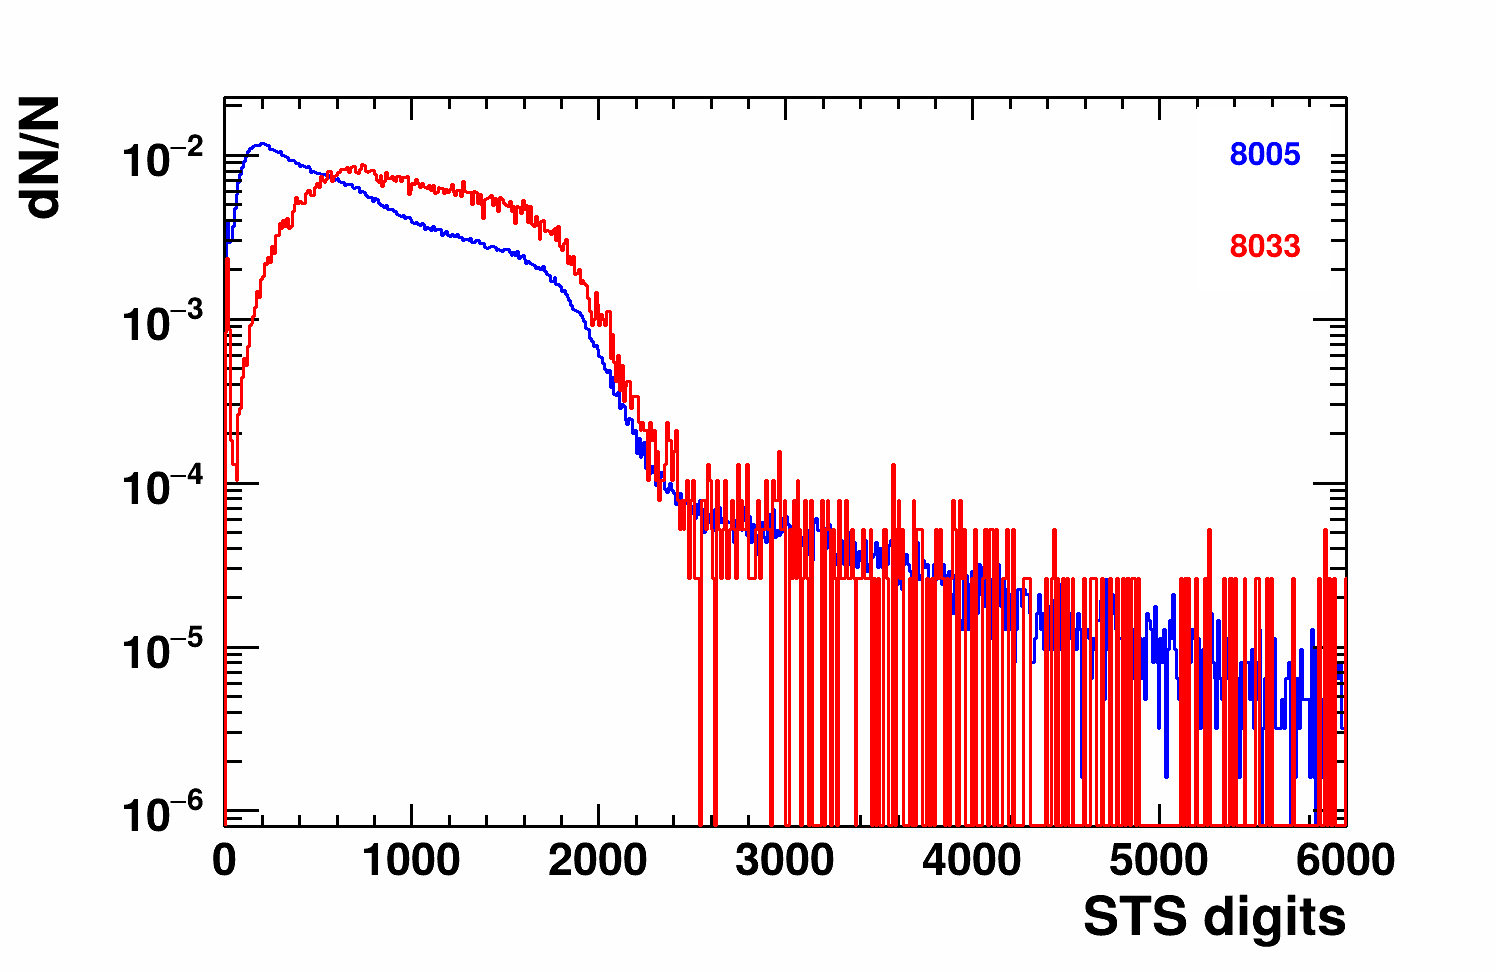
\includegraphics[width=0.35\linewidth]{../pict/QA_RunByRun_24.12/H1/nVtxTr_h2_RunId_stsDigits.png} 
            \label{fig:FSDdigits} }  
        \subfigure[]{
            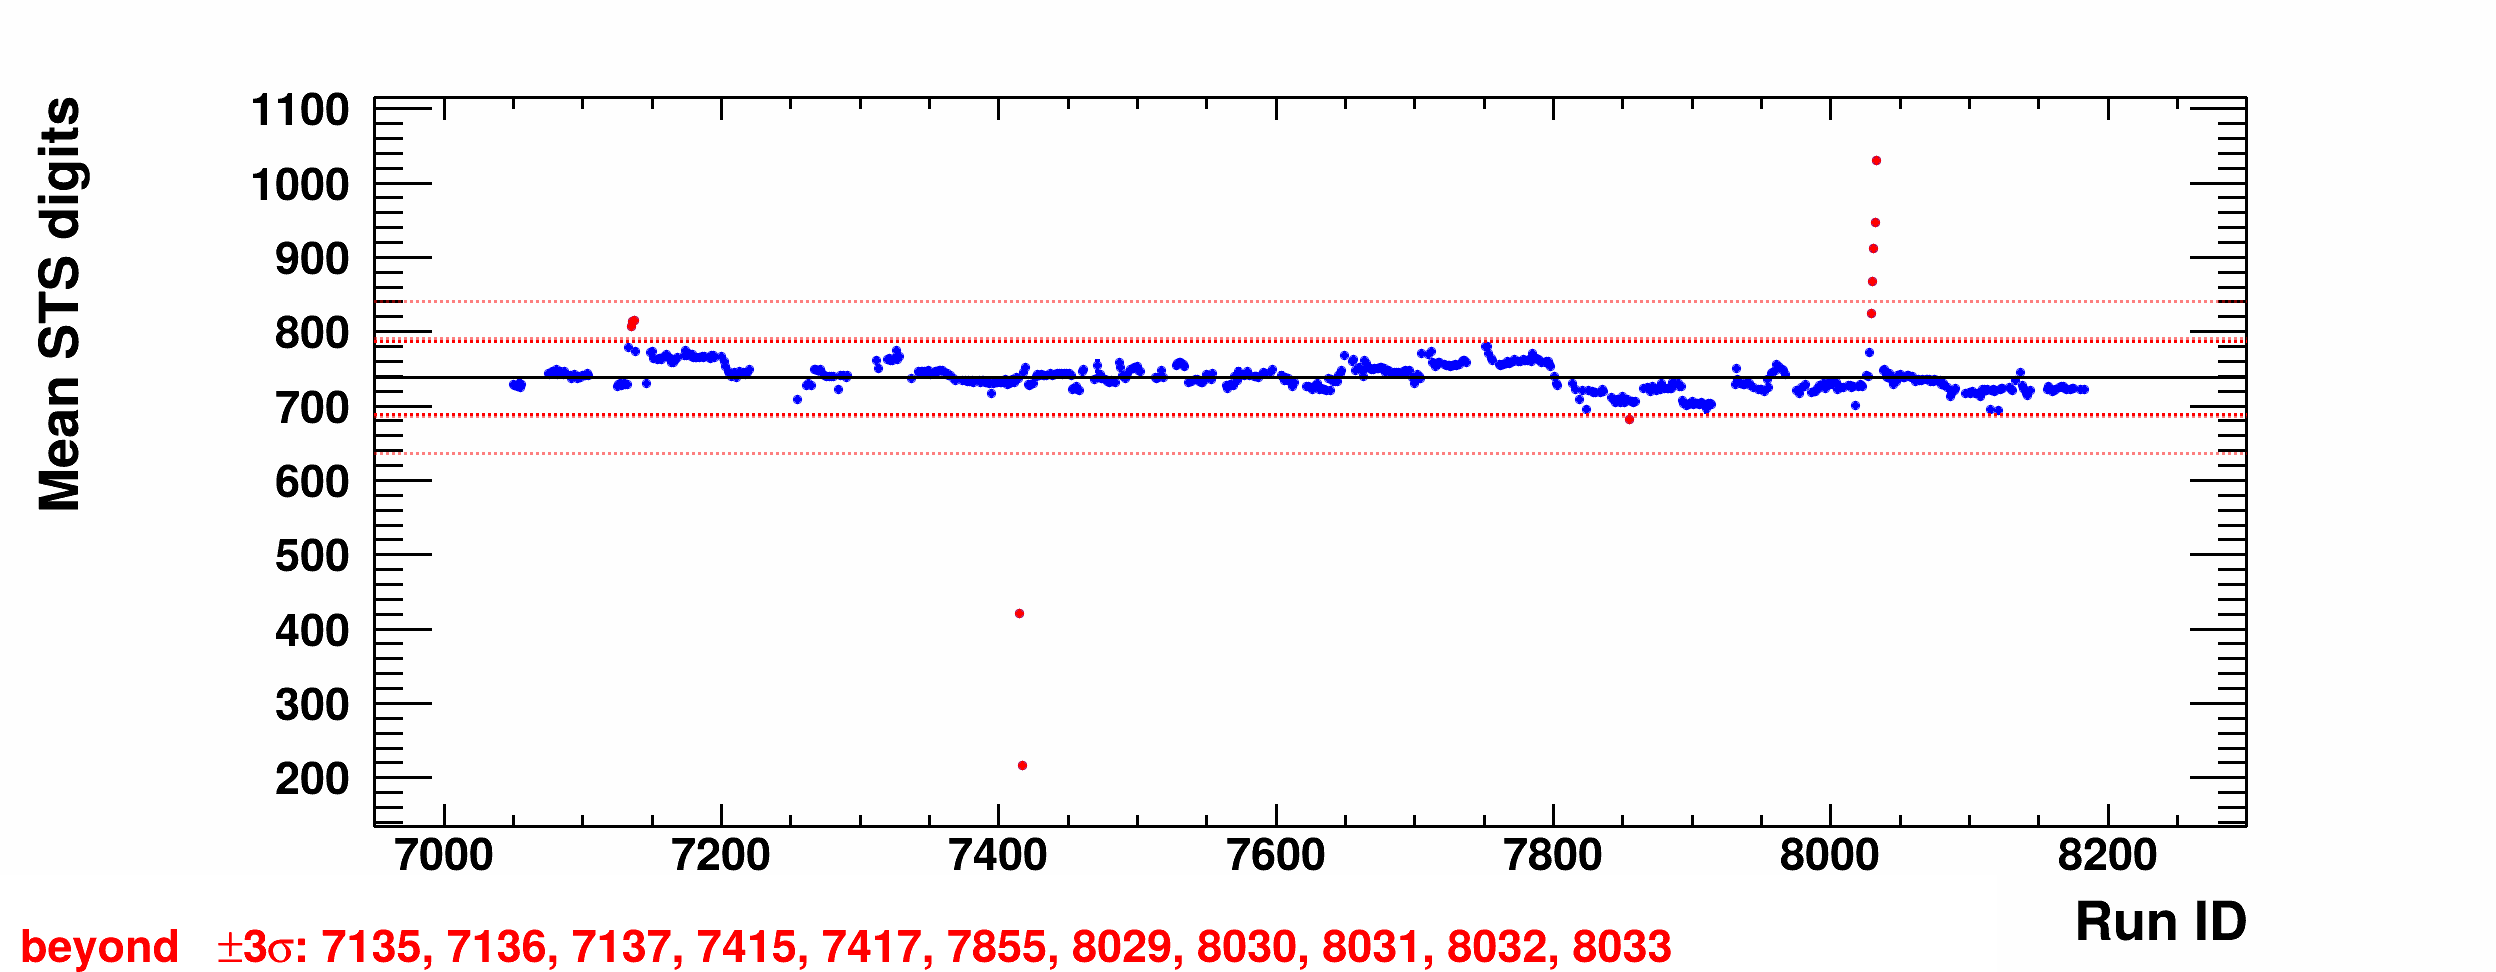
\includegraphics[width=0.60\linewidth]{../pict/QA_RunByRun_24.12/nVtxTr_h2_RunId_stsDigits.png} 
            \label{fig:FSDdigitsRun} }
        \subfigure[]{
            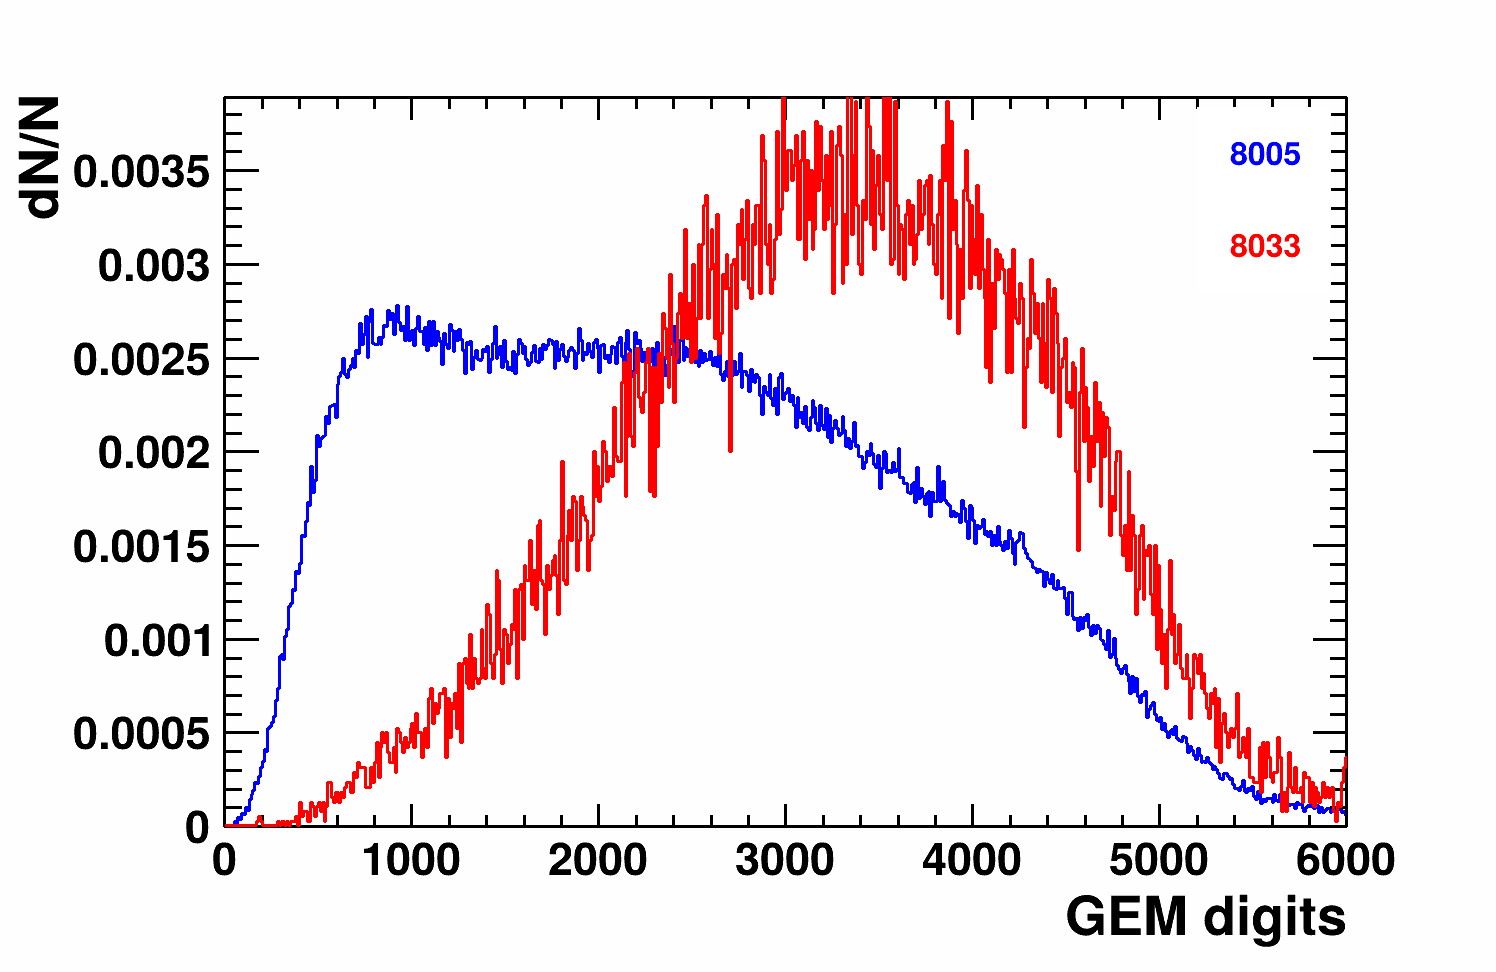
\includegraphics[width=0.35\linewidth]{../pict/QA_RunByRun_24.12/H1/nVtxTr_h2_RunId_gemDigits.png} 
            \label{fig:GEMdigits} }  
        \subfigure[]{
            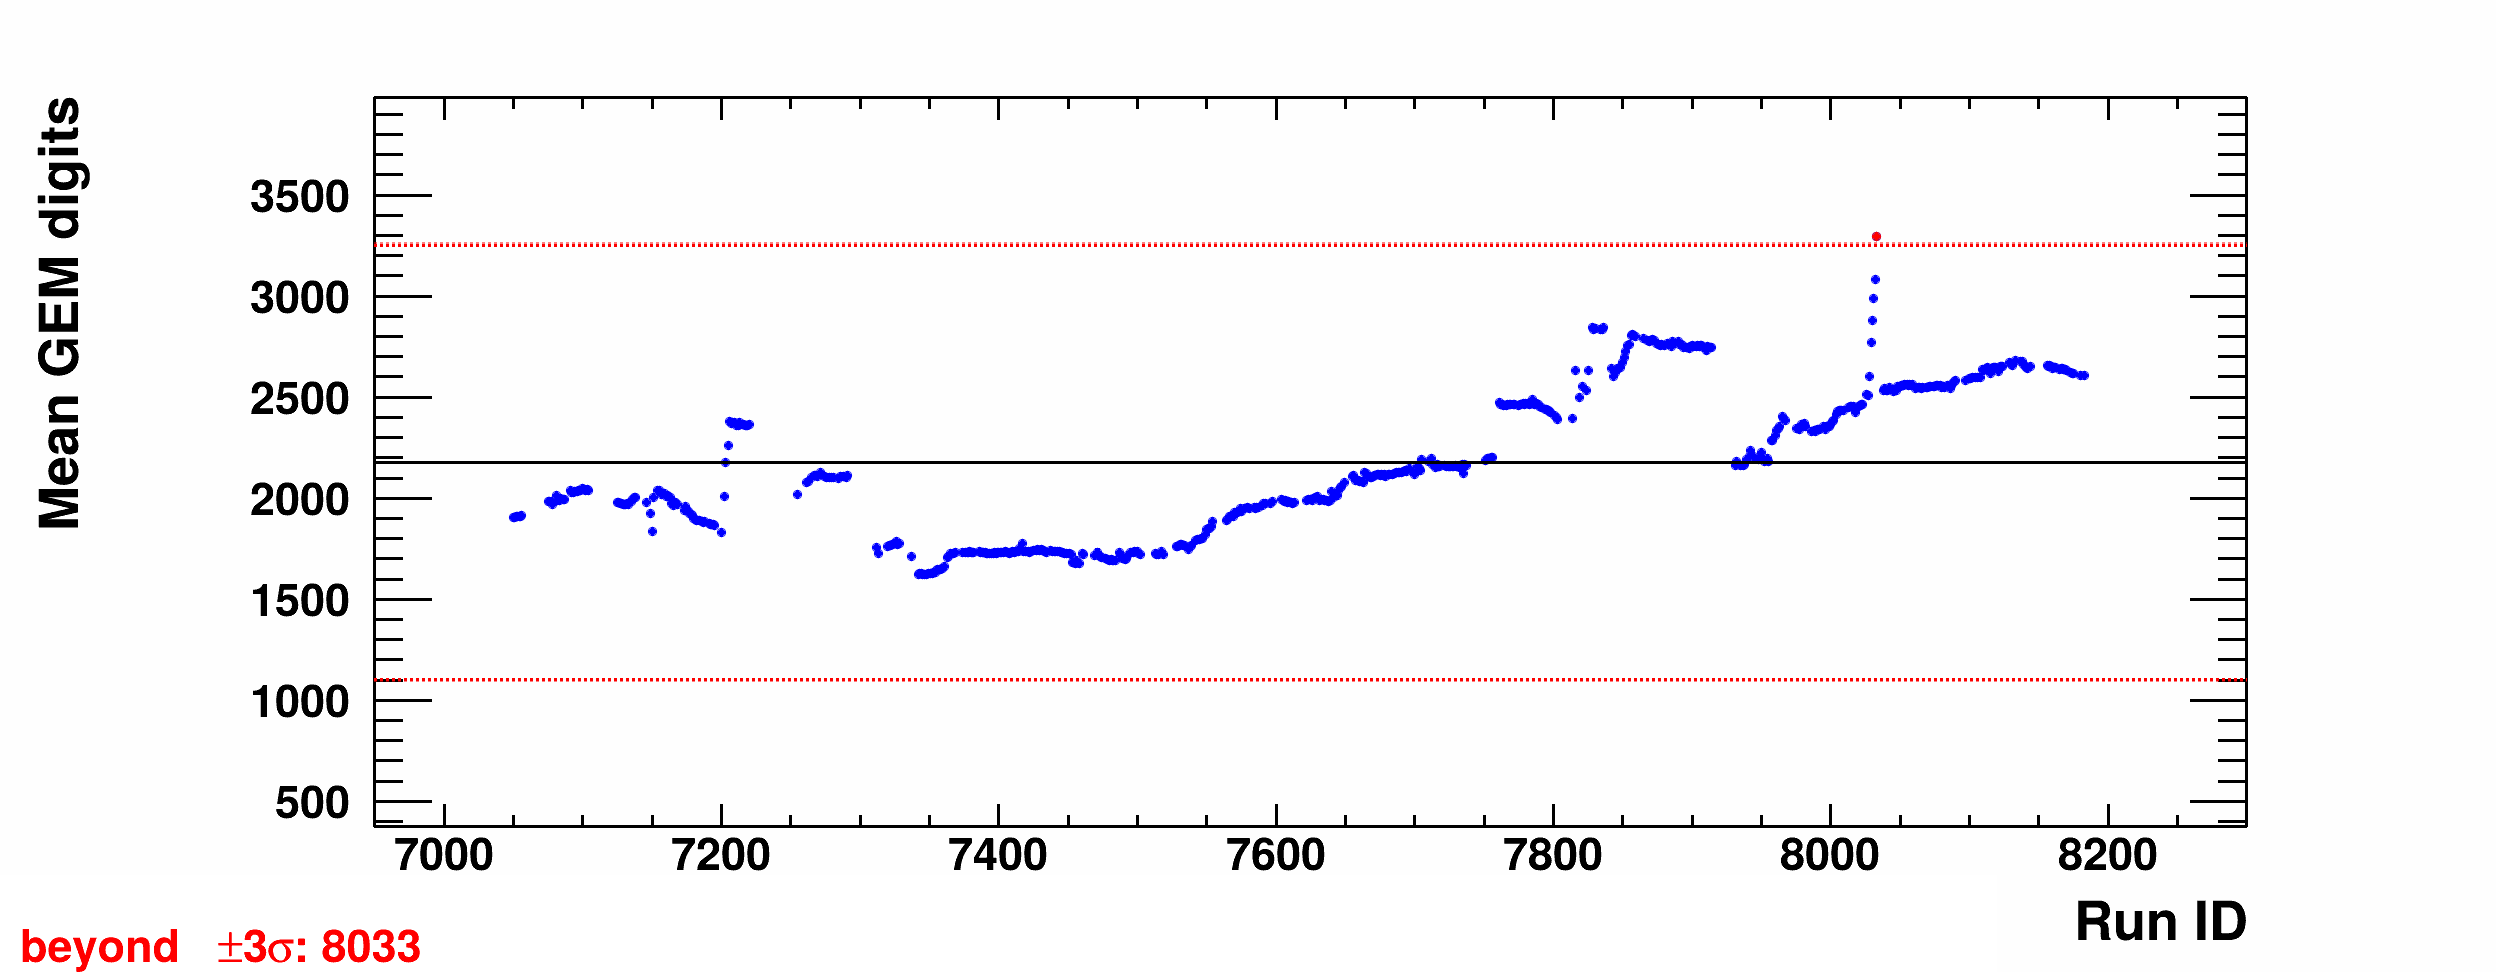
\includegraphics[width=0.60\linewidth]{../pict/QA_RunByRun_24.12/nVtxTr_h2_RunId_gemDigits.png}
            \label{fig:GEMdigitsRun} }
        \vspace{-3mm}
        \caption{Distribution of the number of digits in the FSD \subref{fig:FSDdigits} and GEM \subref{fig:GEMdigits} detector. The red marker corresponds to the distribution from the "outlier" RunId. Mean FSD digits \subref{fig:FSDdigitsRun} and GEM digits \subref{fig:GEMdigitsRun} as a function RunID (right panel). Black dotted horizontal line and red horizontal lines represent $\mu$ and $\pm3\sigma$, respectively.}
        \label{fig:DigitsQA}
        \end{center}
        \vspace{-5mm}
    \end{figure}

    %============================= Fig ================================
    \begin{figure}[H]
        \begin{center}
        \subfigure[]{
            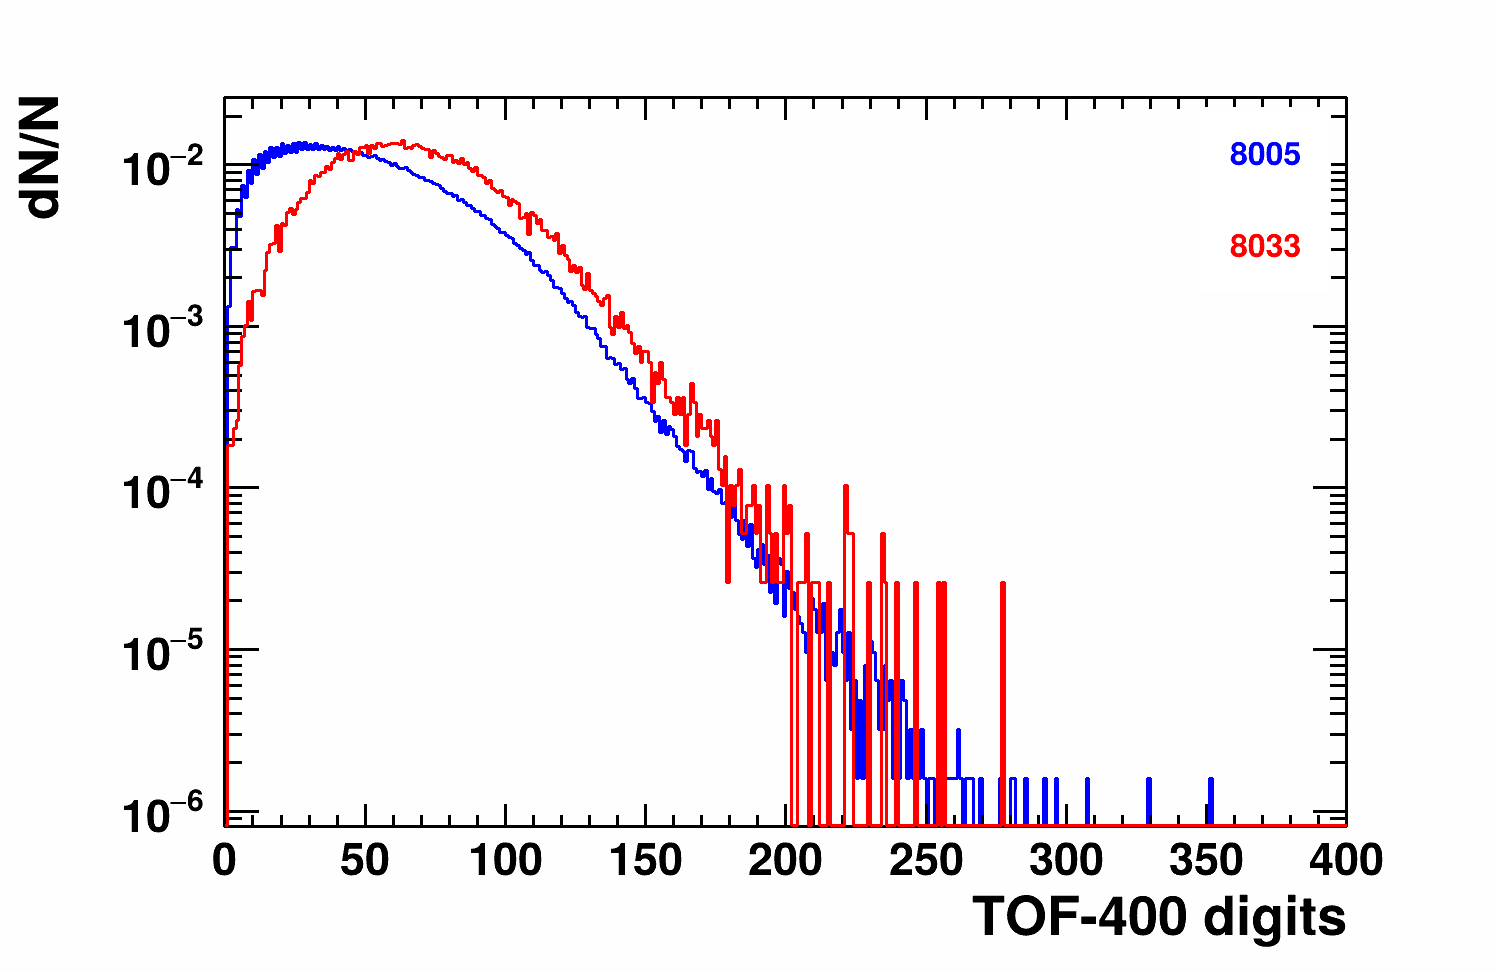
\includegraphics[width=0.35\linewidth]{../pict/QA_RunByRun_24.12/H1/nVtxTr_h2_RunId_tof400Digits.png} 
            \label{fig:TOF400digits} }  
        \subfigure[]{
            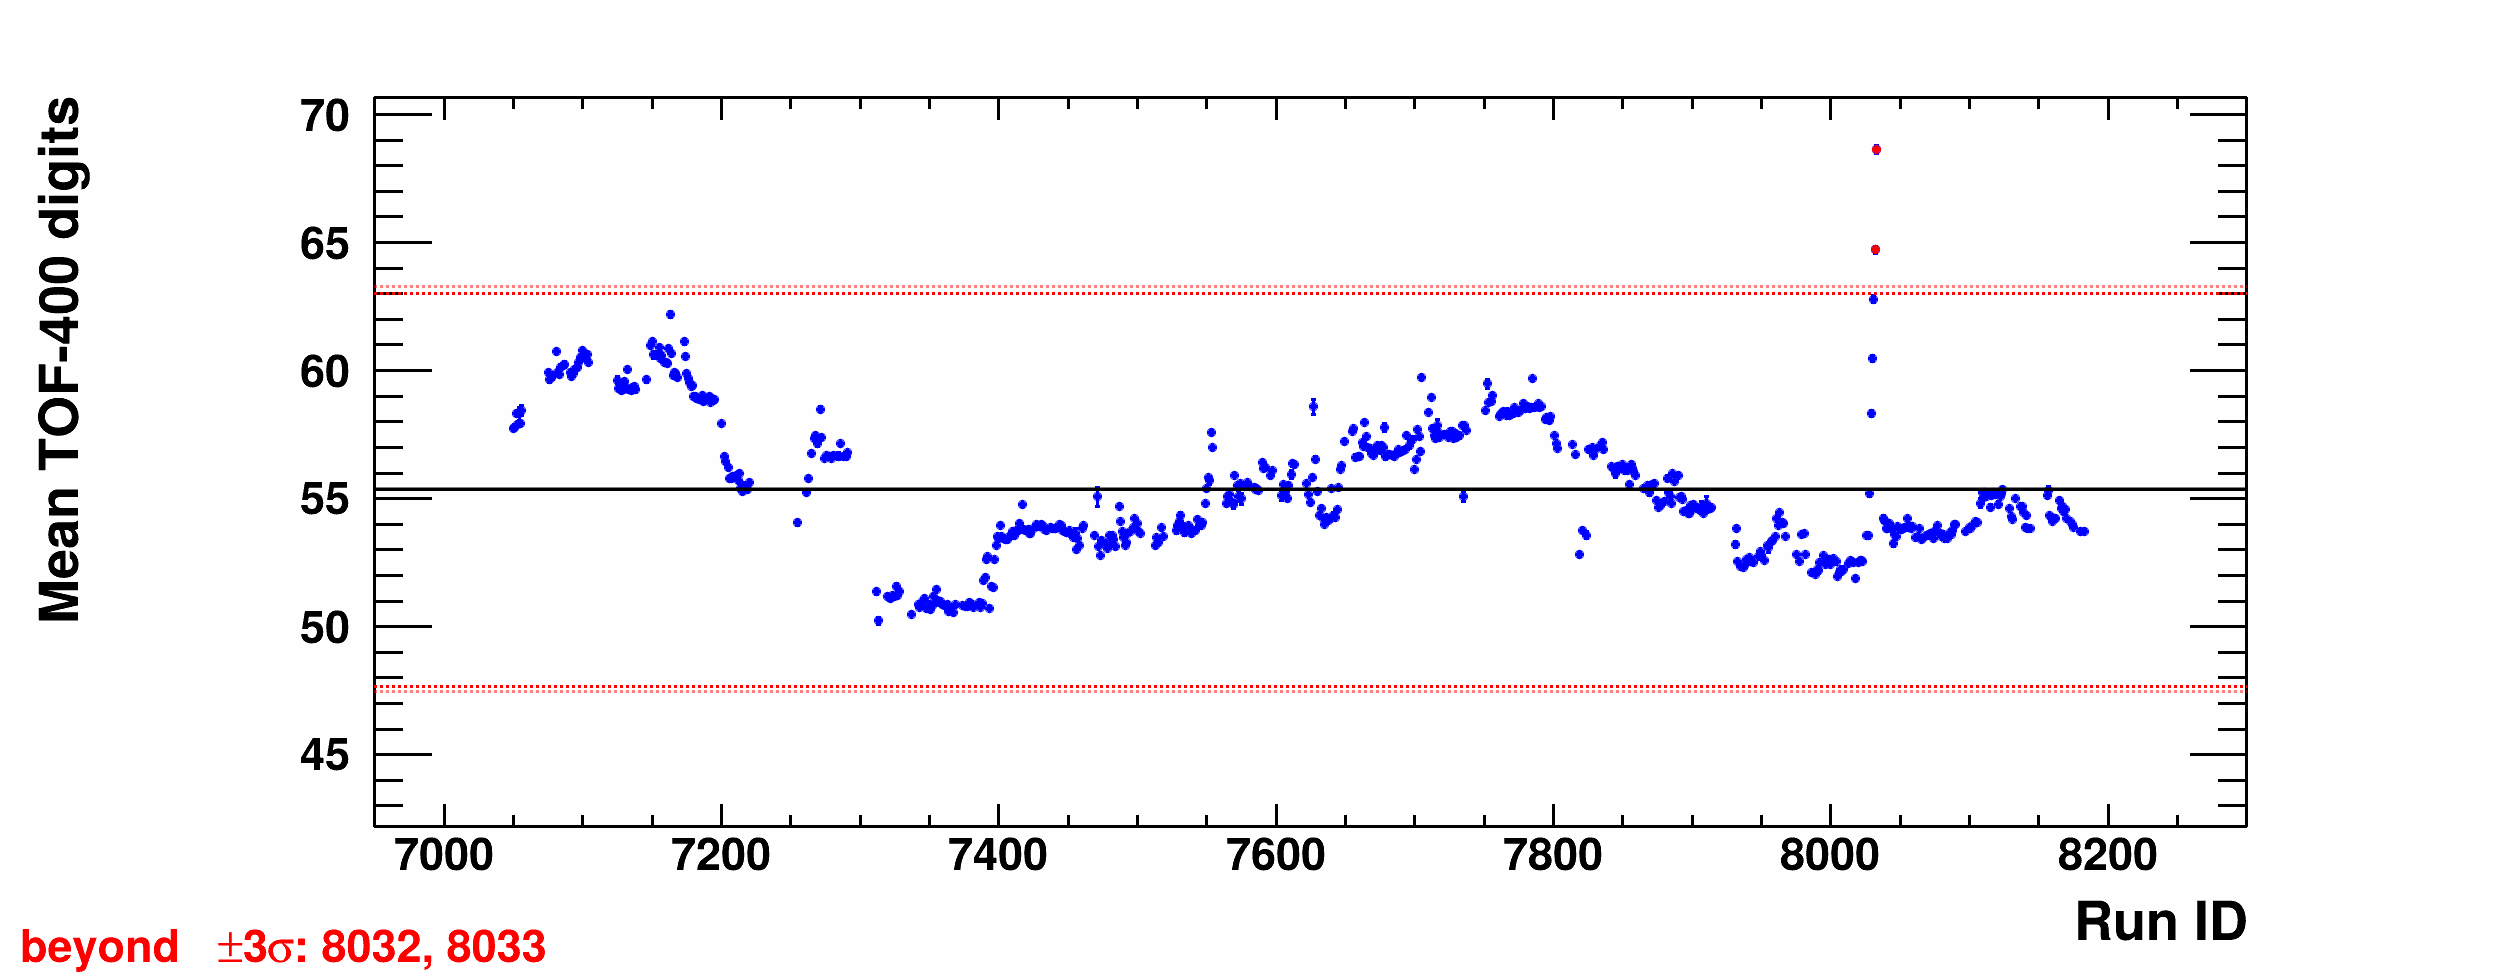
\includegraphics[width=0.60\linewidth]{../pict/QA_RunByRun_24.12/nVtxTr_h2_RunId_tof400Digits.png} 
            \label{fig:TOF400digitsRun} }
        \subfigure[]{
            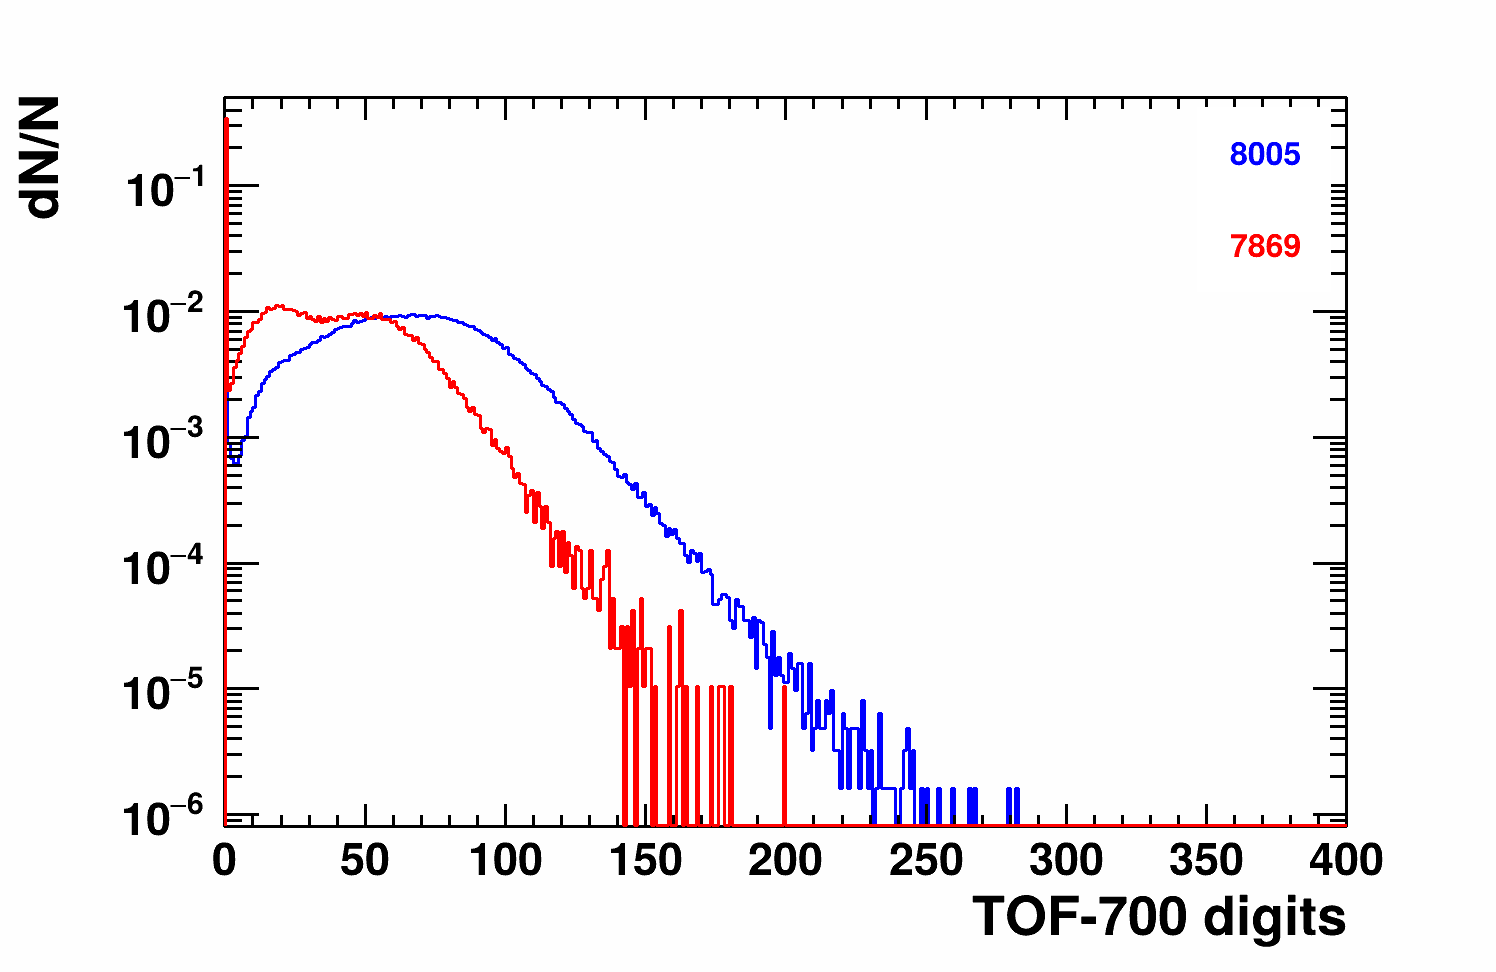
\includegraphics[width=0.35\linewidth]{../pict/QA_RunByRun_24.12/H1/nVtxTr_h2_RunId_tof700Digits.png} 
            \label{fig:TOF700digits} }  
        \subfigure[]{
            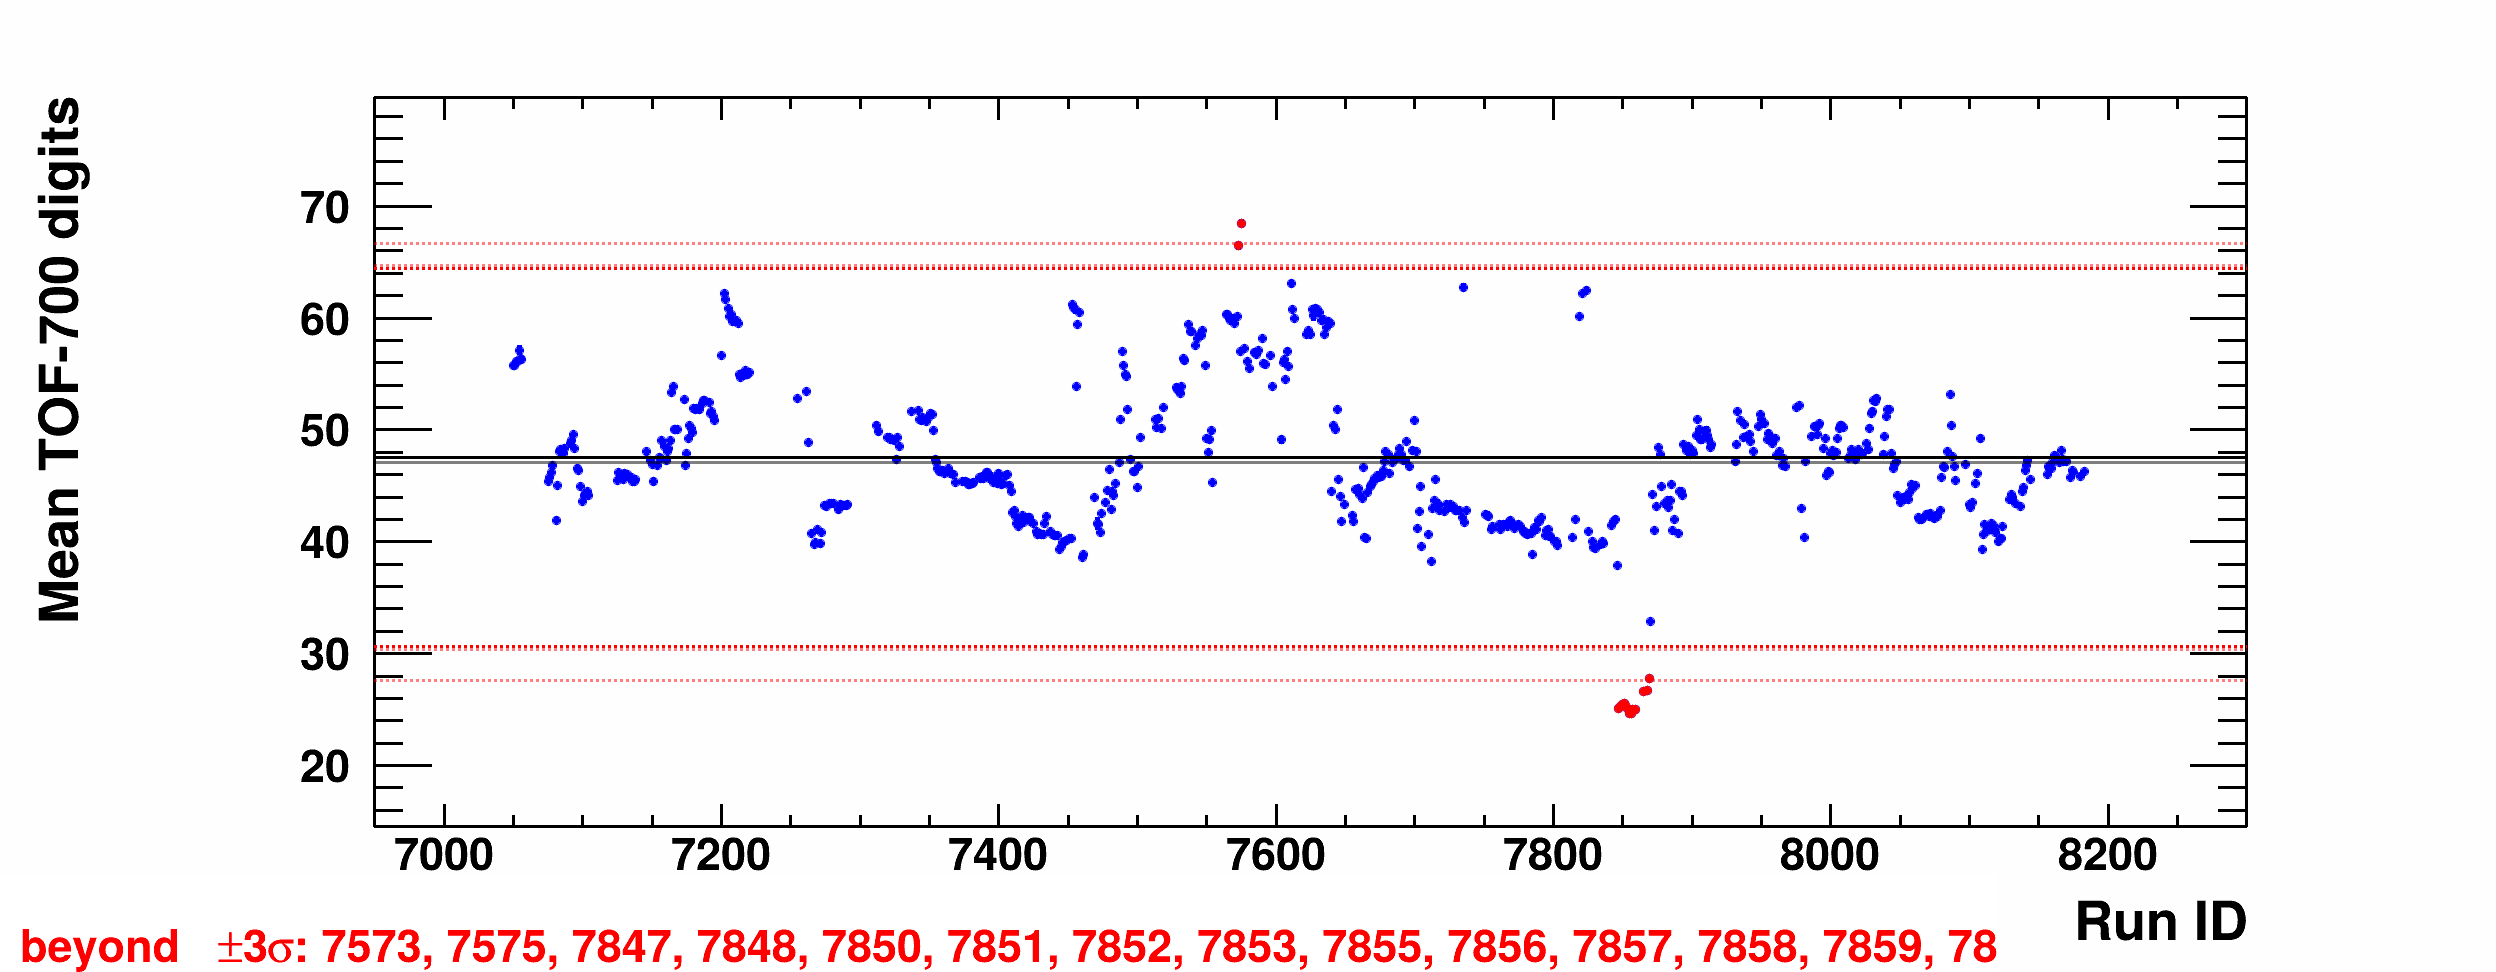
\includegraphics[width=0.60\linewidth]{../pict/QA_RunByRun_24.12/nVtxTr_h2_RunId_tof700Digits.png}
            \label{fig:TOF700digitsRun} }
        \vspace{-3mm}
        \caption{Distribution of the number of digits in the TOF400 \subref{fig:TOF400digits} and TOF700 \subref{fig:TOF700digits} detector. The red marker corresponds to the distribution from the "outlier" RunId. Mean TOF400 digits \subref{fig:TOF400digitsRun} and TOF700 digits \subref{fig:TOF700digitsRun} as a function RunID (right panel). Black dotted horizontal line and red horizontal lines represent $\mu$ and $\pm3\sigma$, respectively.}
        \label{fig:DigitsQA_tof}
        \end{center}
        \vspace{-5mm}
    \end{figure}




\subsection{Vertex position}\label{VtxPosit}
    
    Figure ~\ref{fig:VtxNTracks}-~\ref{fig:VtxChiNdf} shows the RunId dependence of the mean number of tracks used in the vertex reconstruction and $\chi^2$/NDF. Figure ~\ref{fig:Vertex} shows the RunId dependence of the mean x, y and z positions of the reconstructed vertex.

    %============================= Fig ================================
    \begin{figure}[H]
        \begin{center}
            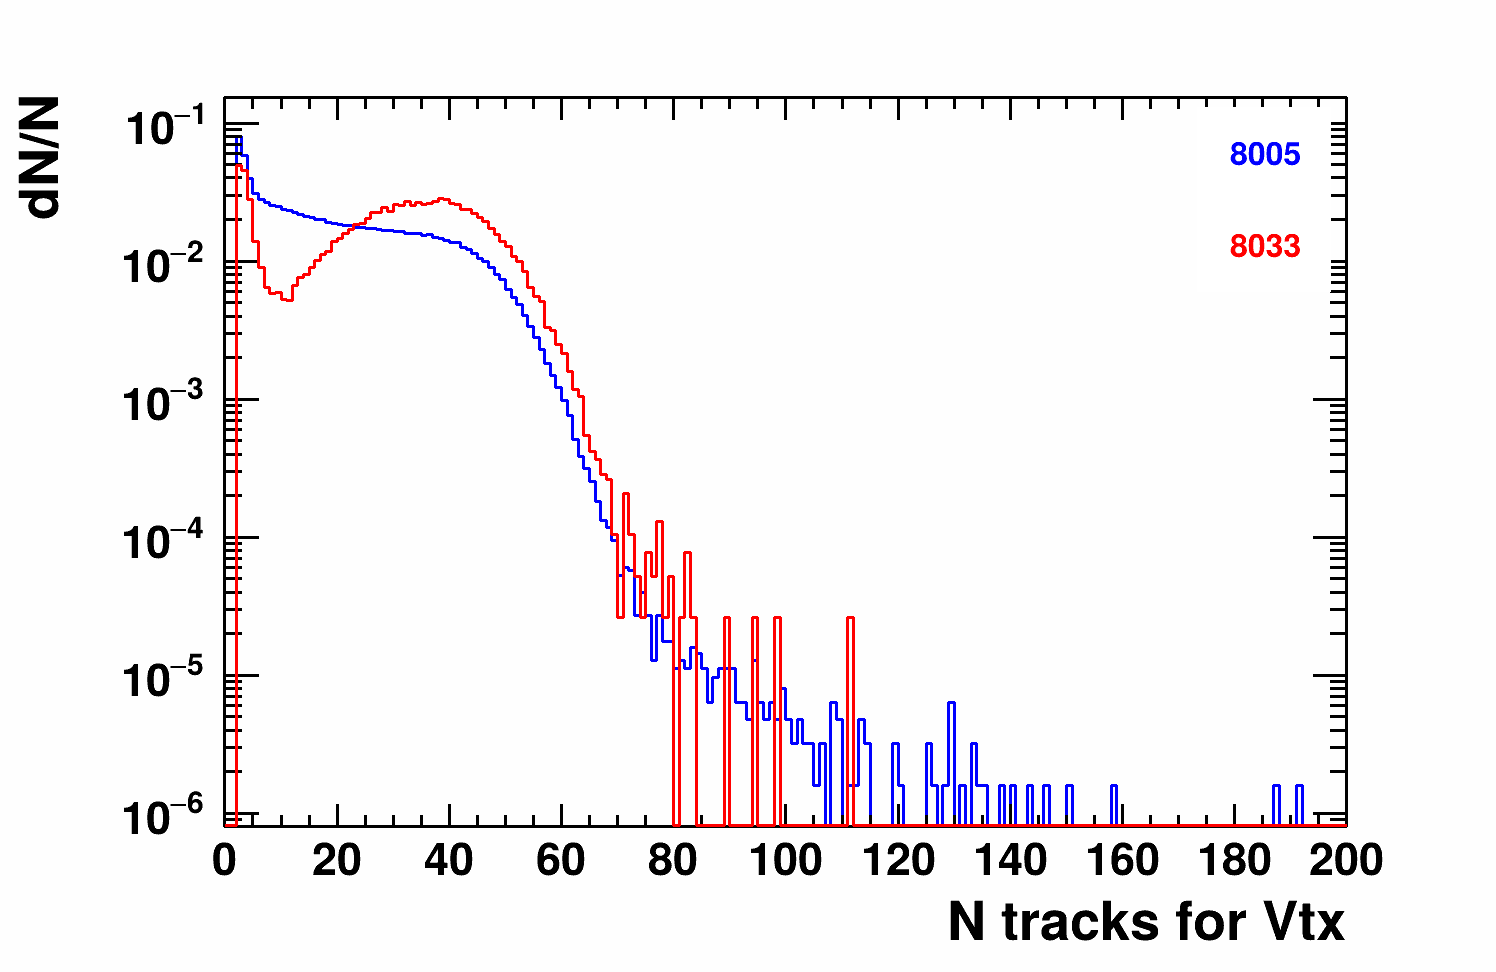
\includegraphics[width=0.35\linewidth]{../pict/QA_RunByRun_24.12/H1/nVtxTr_h2_RunId_vtx_n_tracks.png}
            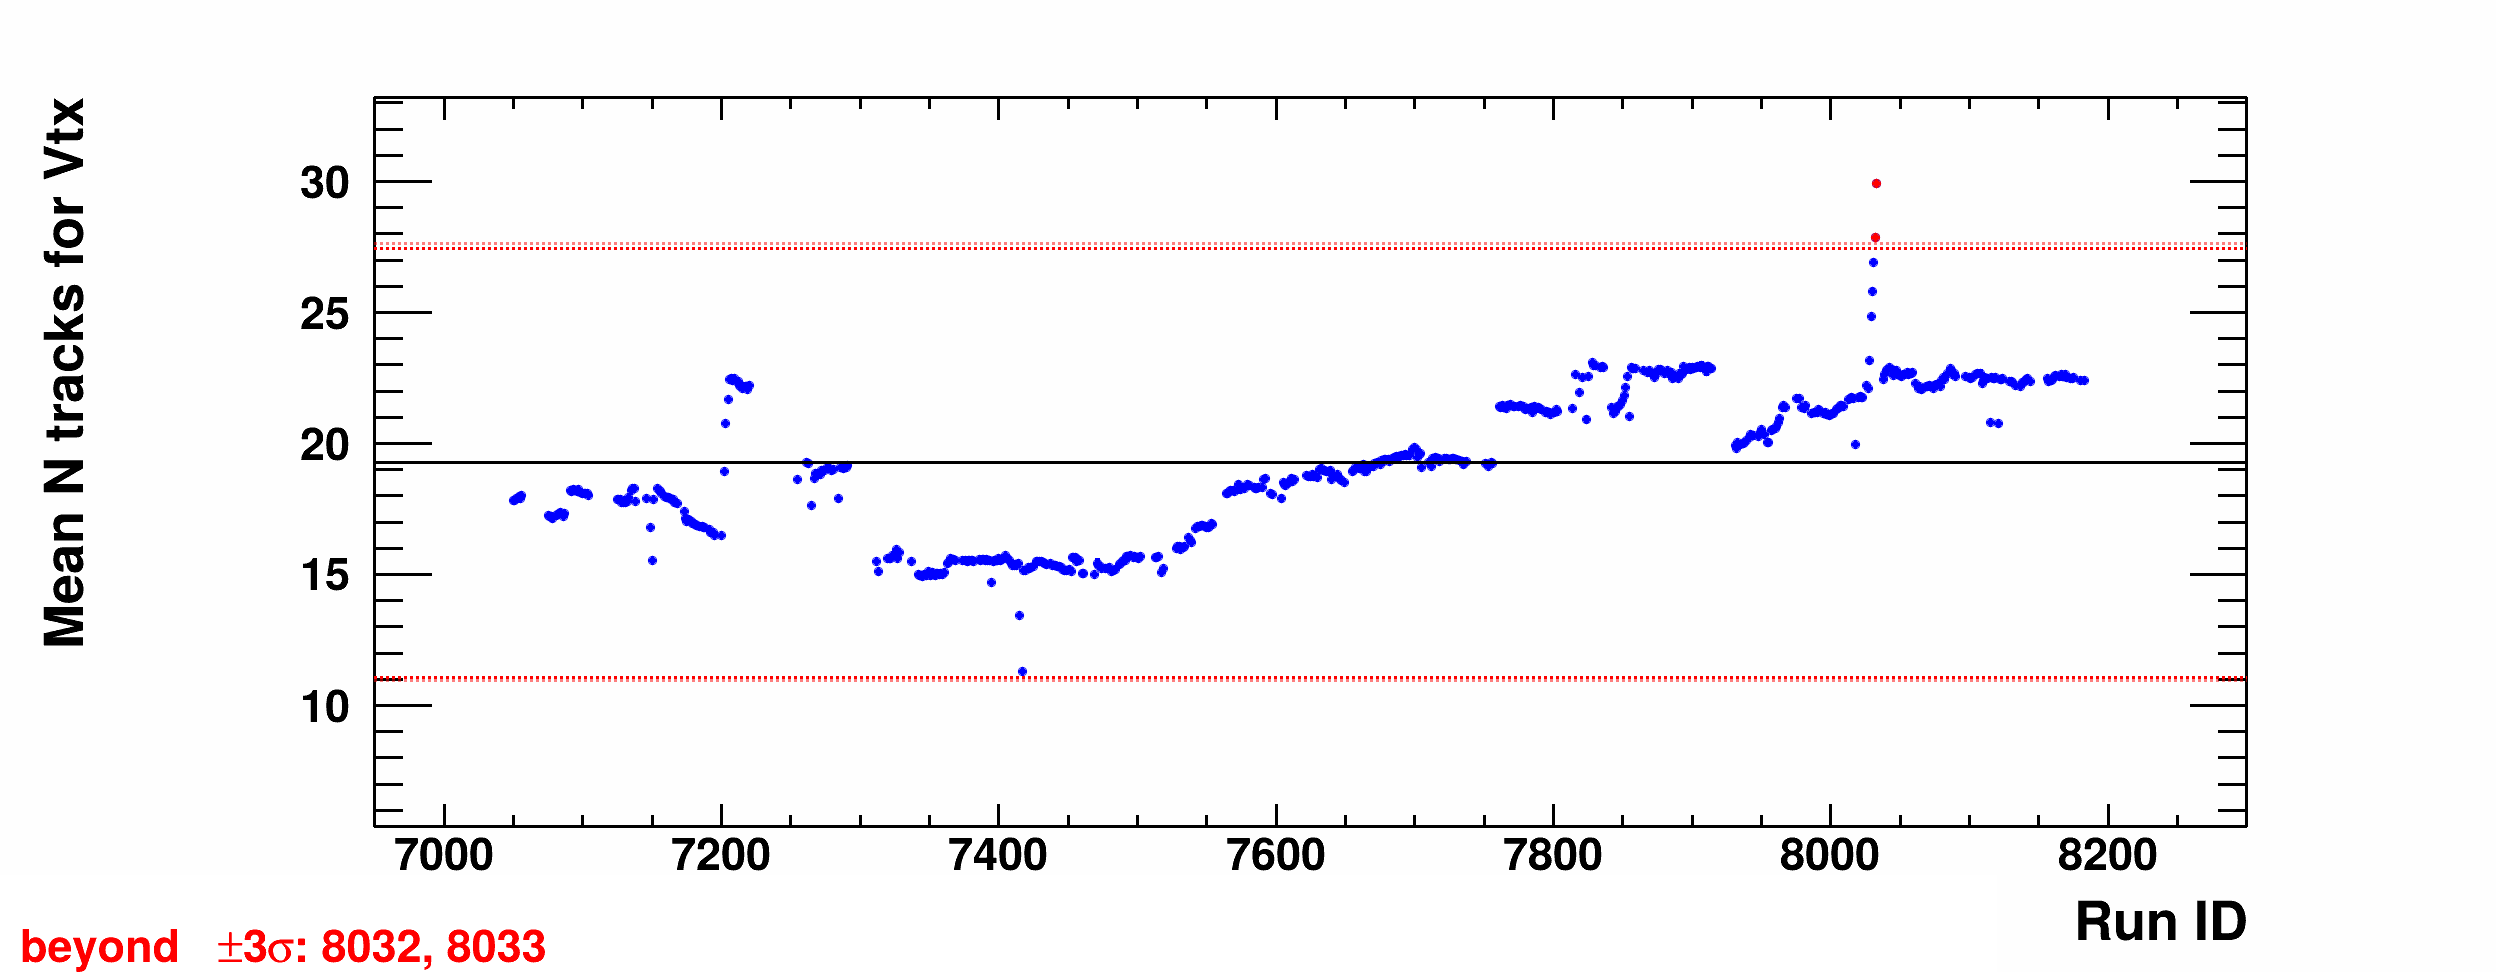
\includegraphics[width=0.60\linewidth]{../pict/QA_RunByRun_24.12/nVtxTr_h2_RunId_vtx_n_tracks.png}
            \vspace{-3mm}
            \caption{Left panel: distribution of the number of track in vertex reconstruction. The red marker corresponds to the distribution from the "outlier" RunId. Right panel: Mean the number of track in vertex reconstruction as a function RunID. Black dotted horizontal line and red horizontal lines represent $\mu$ and $\pm3\sigma$, respectively.}
            \label{fig:VtxNTracks}
        \end{center}
        \vspace{-5mm}
    \end{figure}

    %============================= Fig ================================
    \begin{figure}[H]
        \begin{center}
            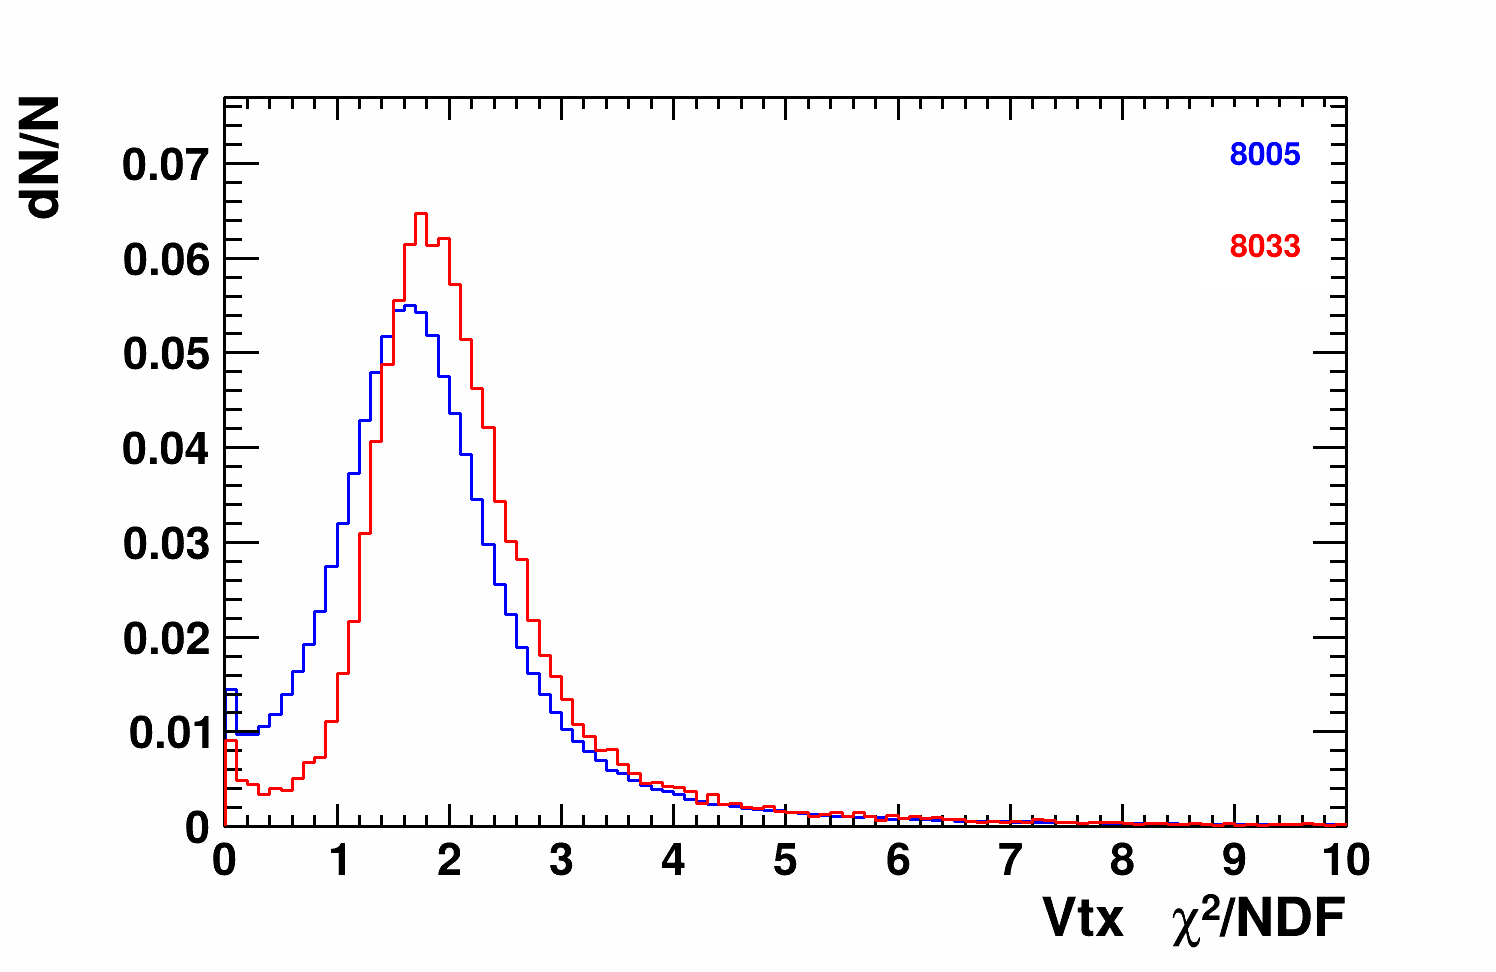
\includegraphics[width=0.35\linewidth]{../pict/QA_RunByRun_24.12/H1/nVtxTr_h2_RunId_vtx_chi2_ndf.png}
            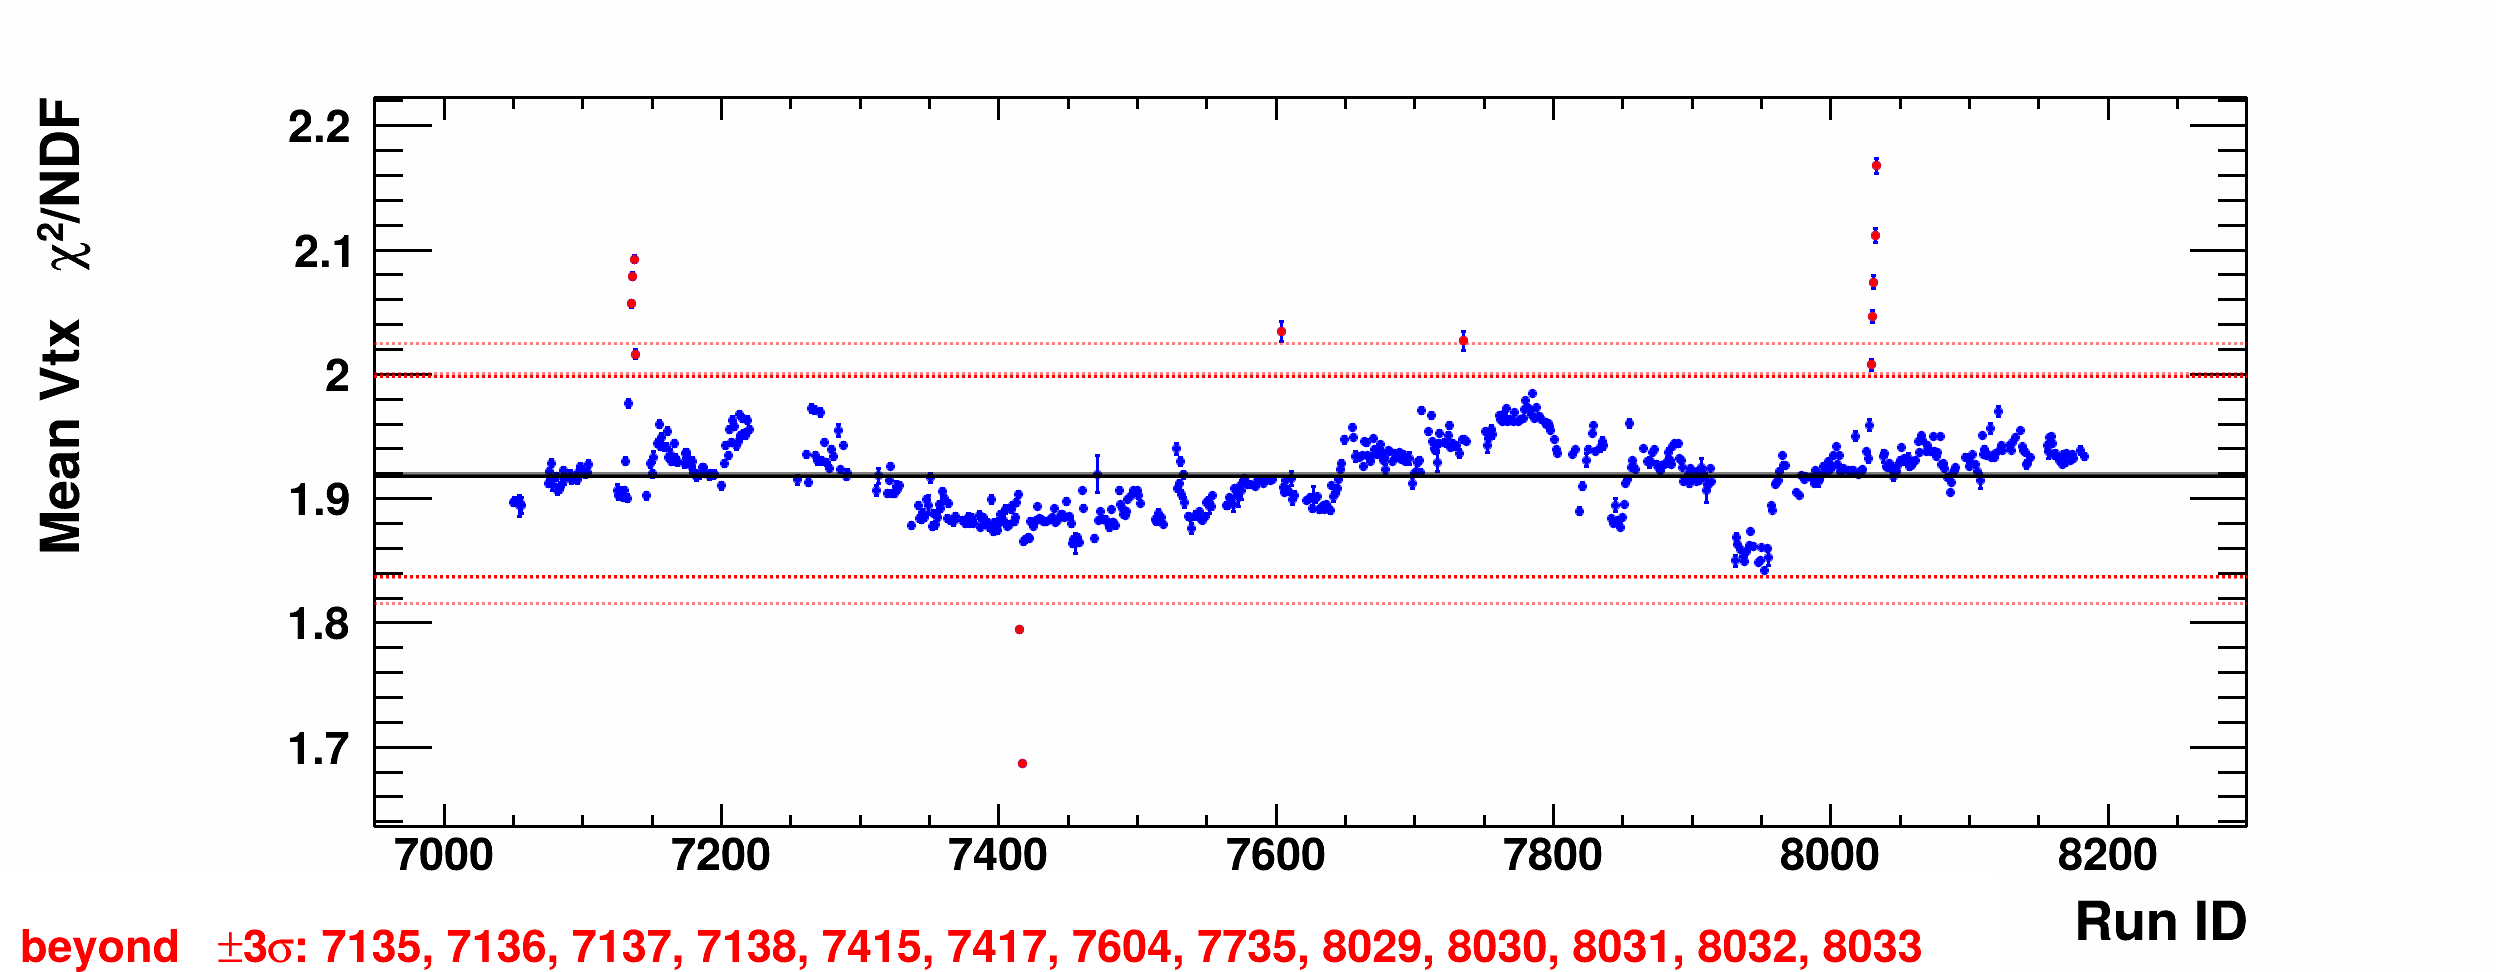
\includegraphics[width=0.60\linewidth]{../pict/QA_RunByRun_24.12/nVtxTr_h2_RunId_vtx_chi2_ndf.png}
            \vspace{-3mm}
            \caption{Left panel: distribution of $\chi^2$/NDF for vertex reconstruction. The red marker corresponds to the distribution from the "outlier" RunId. Right panel: Mean $\chi^2$/NDF for vertex reconstruction as a function RunID. Black dotted horizontal line and red horizontal lines represent $\mu$ and $\pm3\sigma$, respectively.}
            \label{fig:VtxChiNdf}
        \end{center}
        \vspace{-5mm}
    \end{figure}

    %============================= Fig ================================
    \begin{figure}[H]
        \begin{center}
            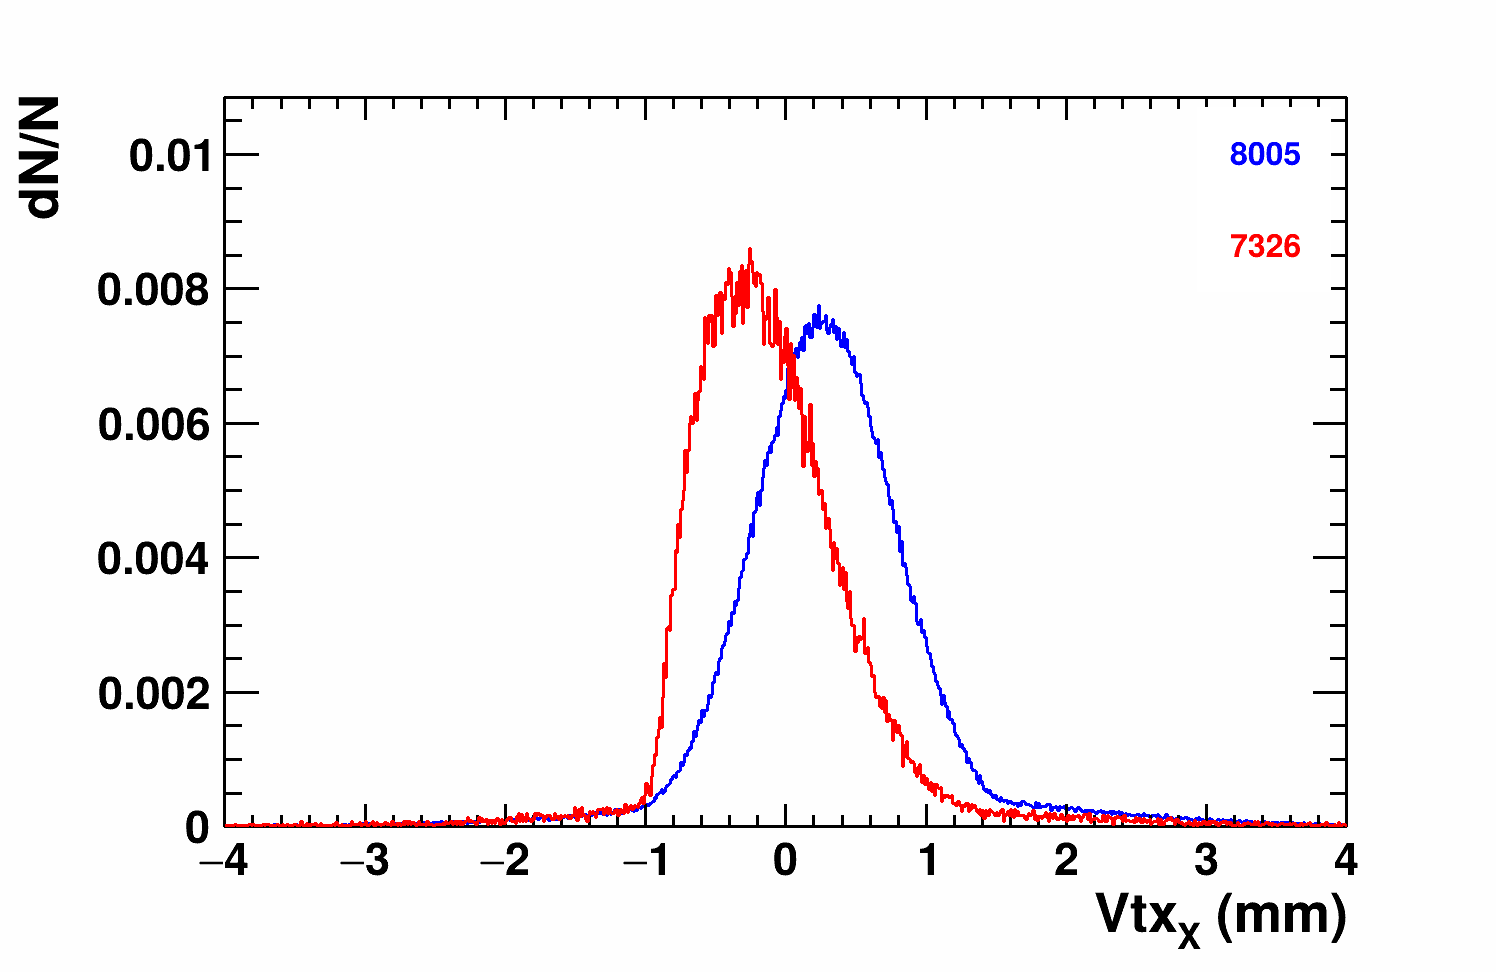
\includegraphics[width=0.35\linewidth]{../pict/QA_RunByRun_24.12/H1/nVtxTr_h2_RunId_vtx_x.png}
            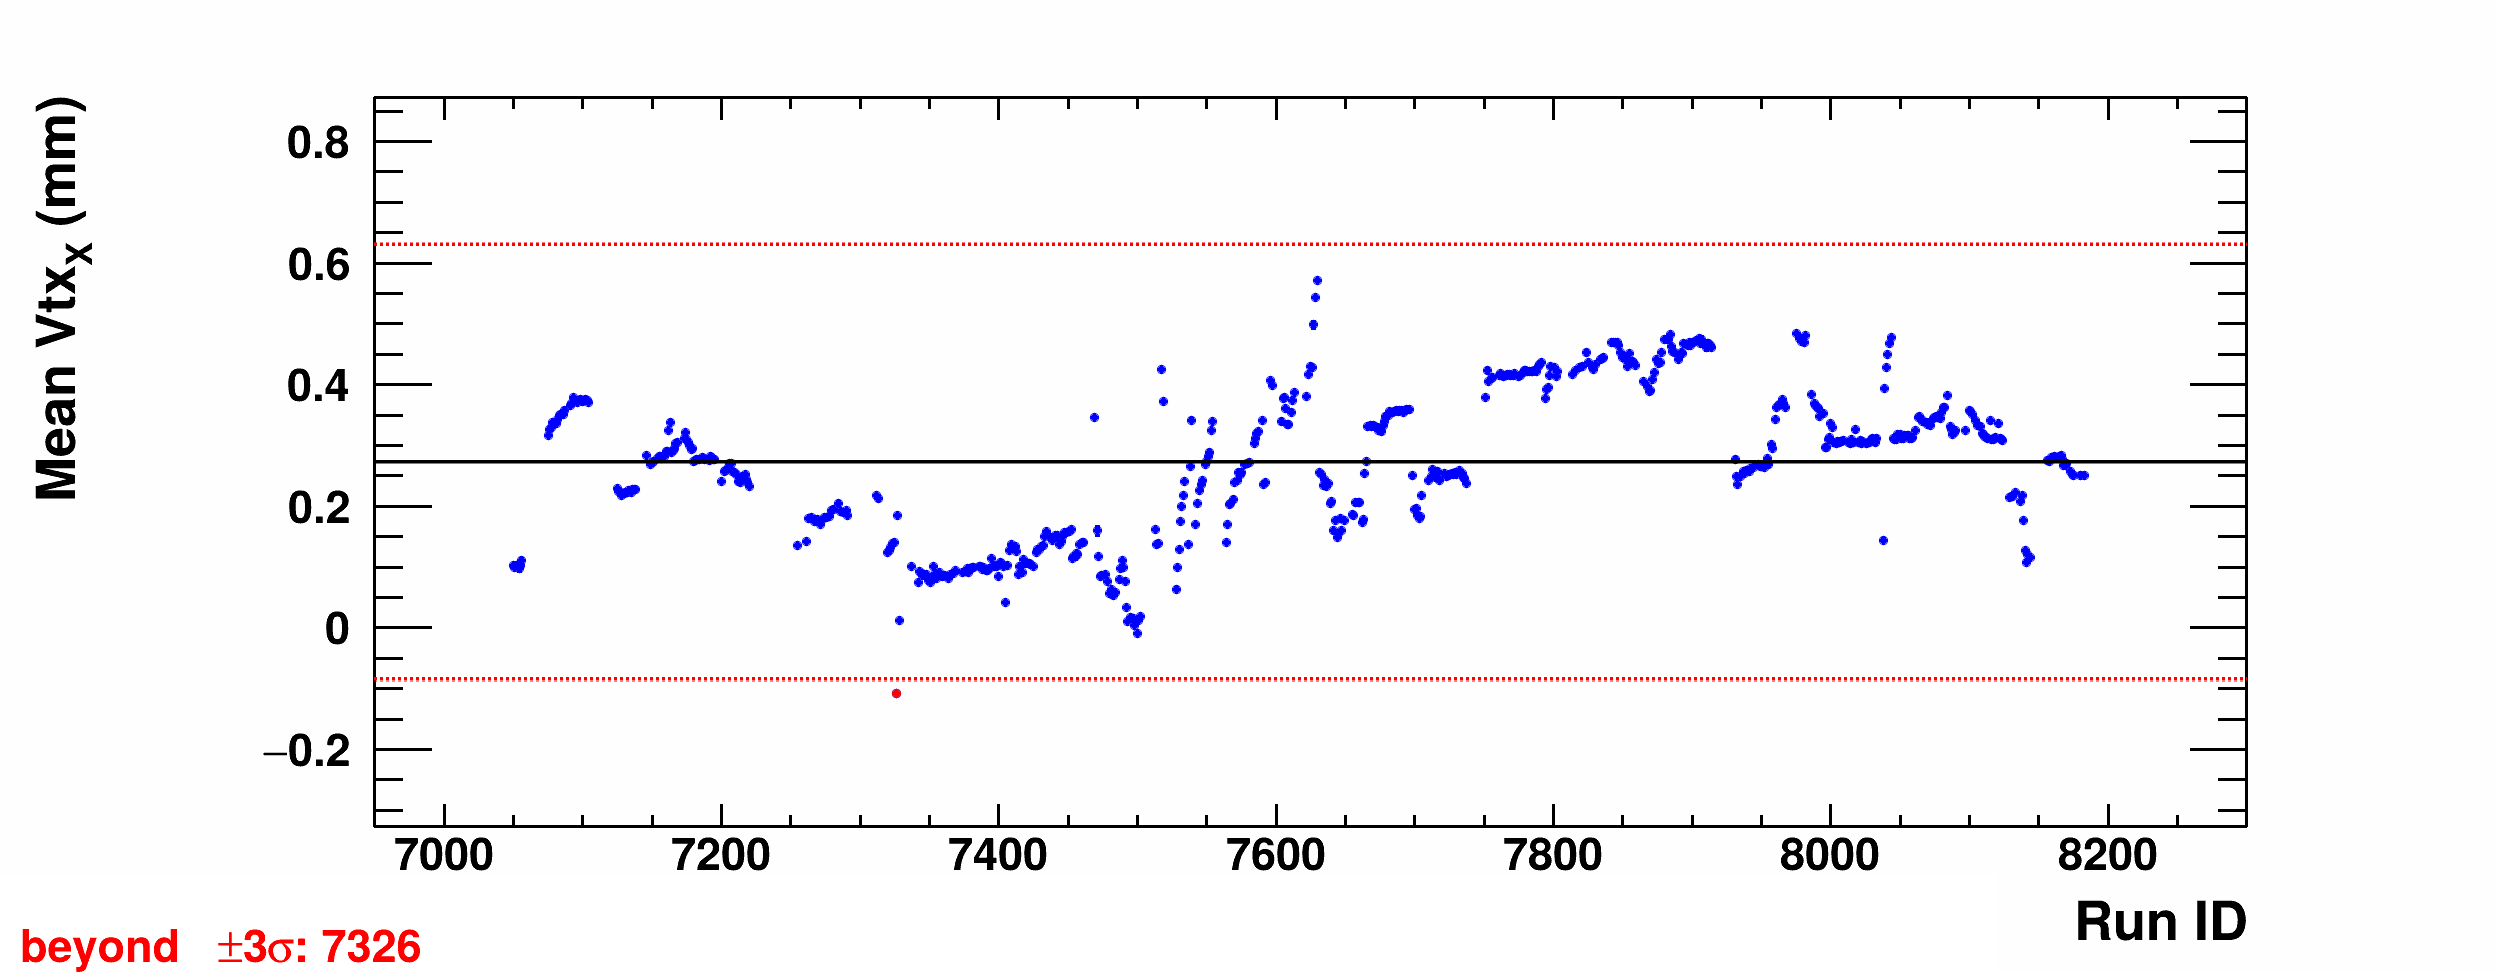
\includegraphics[width=0.60\linewidth]{../pict/QA_RunByRun_24.12/nVtxTr_h2_RunId_vtx_x.png}

            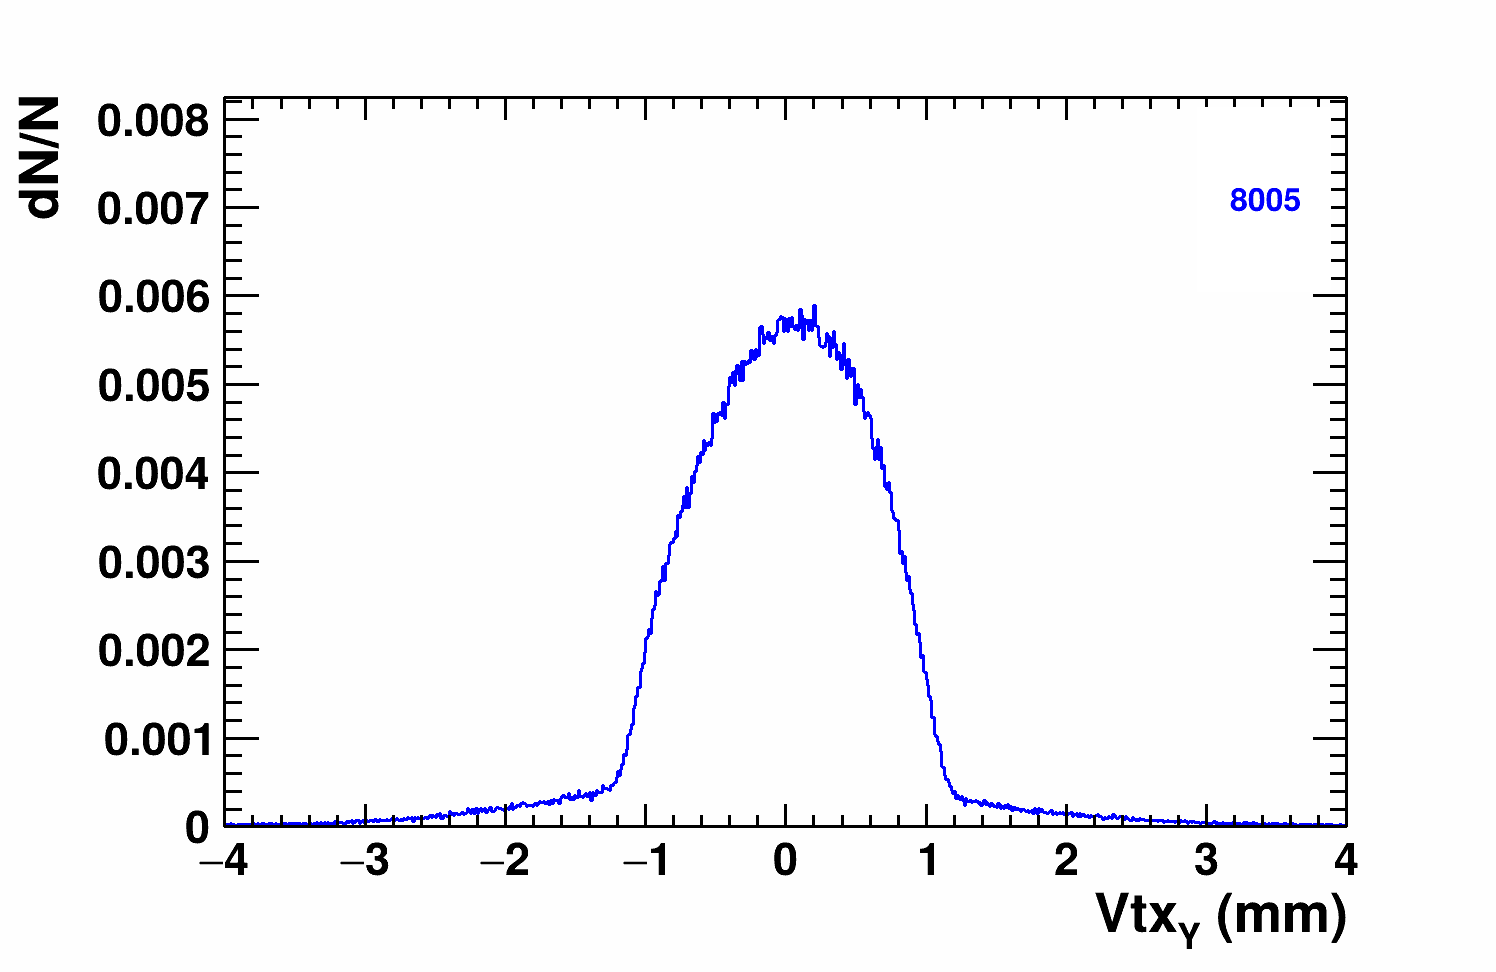
\includegraphics[width=0.35\linewidth]{../pict/QA_RunByRun_24.12/H1/nVtxTr_h2_RunId_vtx_y.png}
            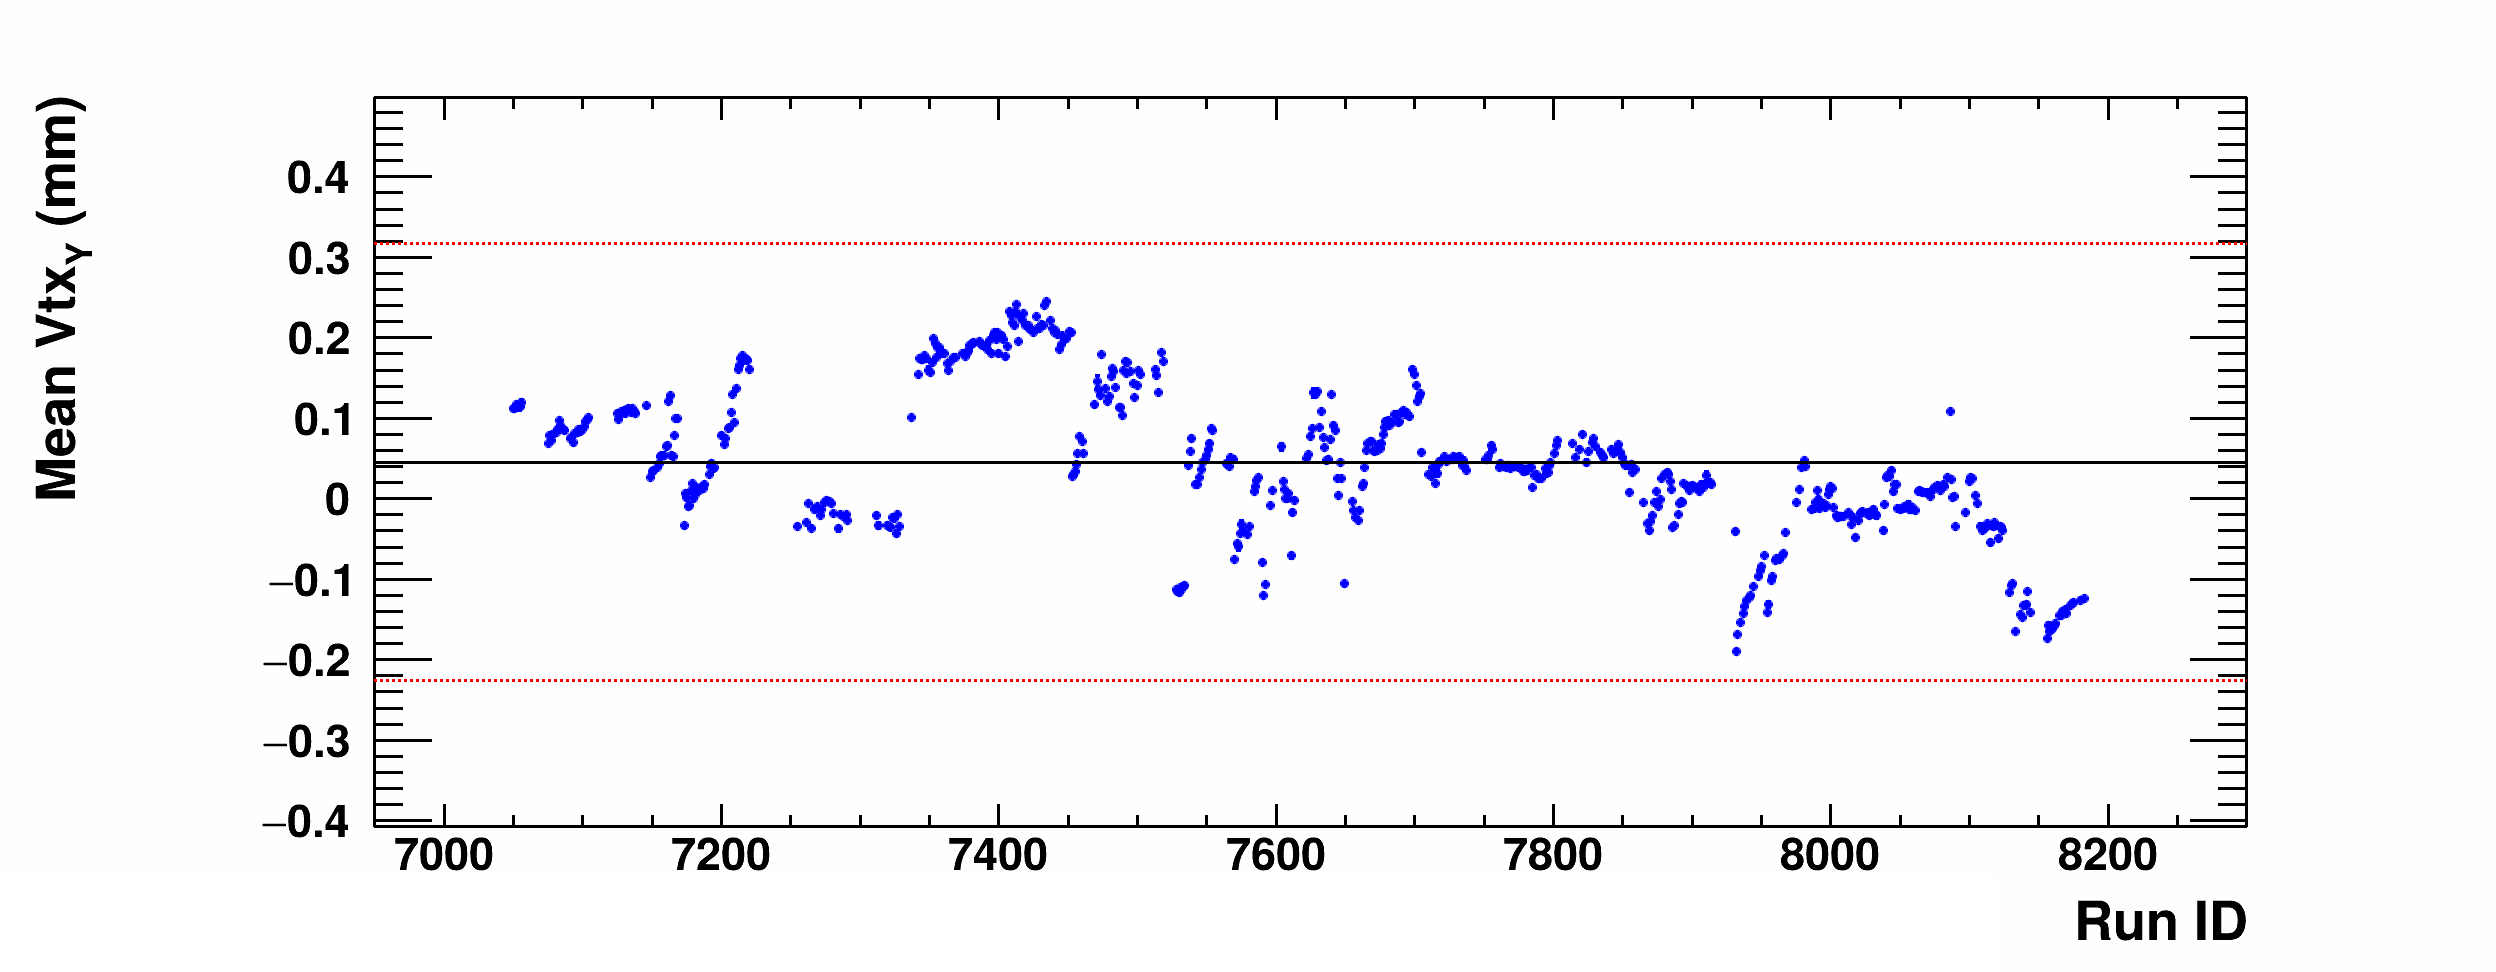
\includegraphics[width=0.60\linewidth]{../pict/QA_RunByRun_24.12/nVtxTr_h2_RunId_vtx_y.png}

            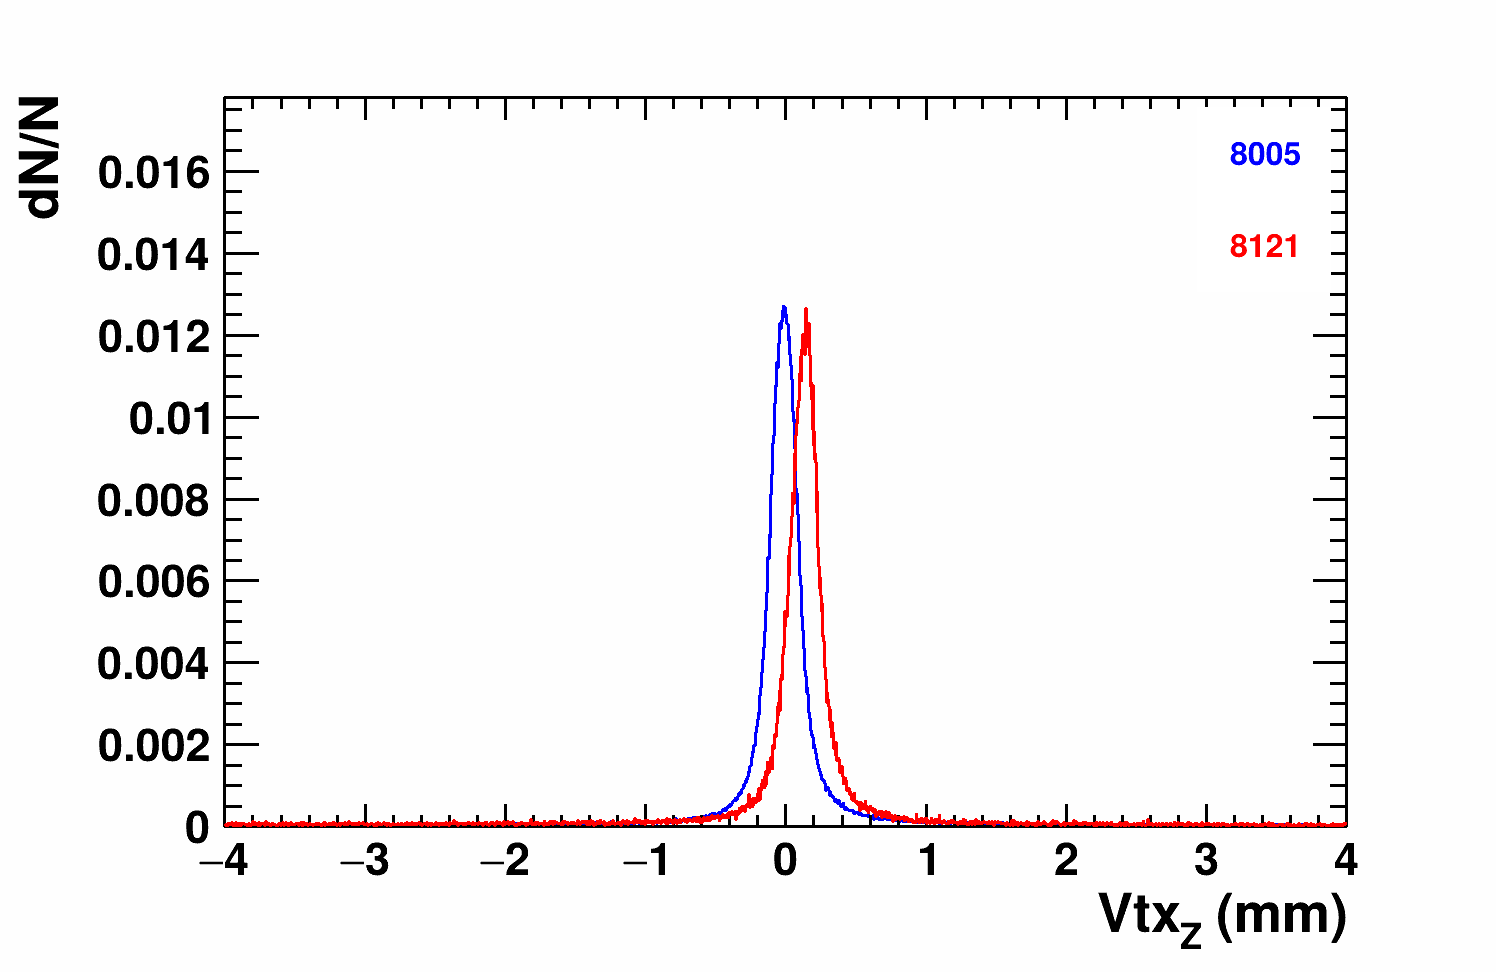
\includegraphics[width=0.35\linewidth]{../pict/QA_RunByRun_24.12/H1/nVtxTr_h2_RunId_vtx_z.png}
            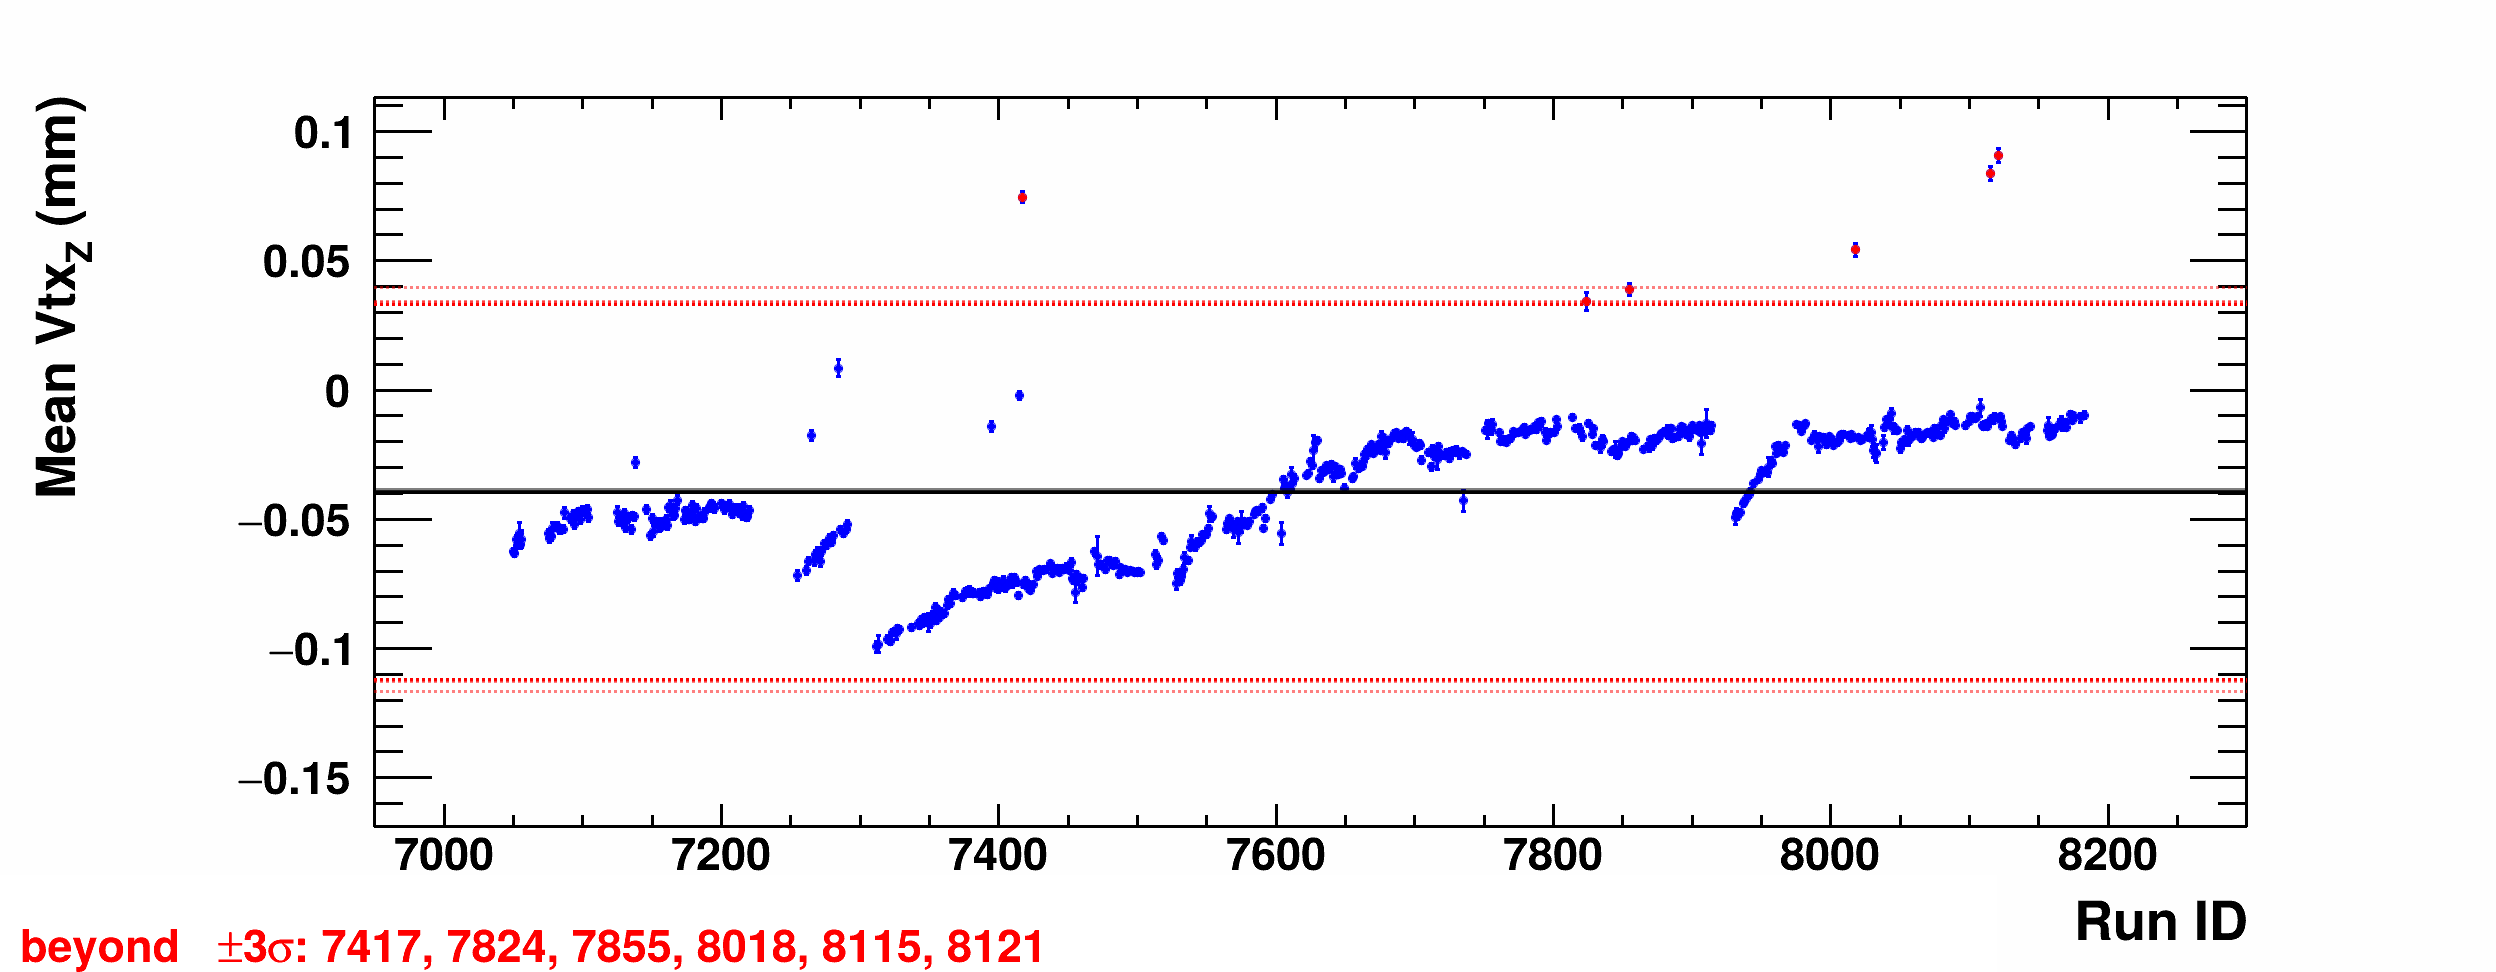
\includegraphics[width=0.60\linewidth]{../pict/QA_RunByRun_24.12/nVtxTr_h2_RunId_vtx_z.png}

            \vspace{-3mm}
            \caption{Left panels: distribution of the x,y and z positions of vertex. The red marker corresponds to the distribution from the "outlier" RunId. Right panels: Mean of the x,y and z positions of vertex as a function RunID. Black dotted horizontal line and red horizontal lines represent $\mu$ and $\pm3\sigma$, respectively.}
            \label{fig:Vertex}
        \end{center}
        \vspace{-5mm}
    \end{figure}




\subsection{Multiplicity}

    Figure ~\ref{fig:mult} shows the RunId dependence of the mean multiplicity of charged particles in the tracking system (FSD + GEM).

    %============================= Fig ================================
    \begin{figure}[H]
        \begin{center}
            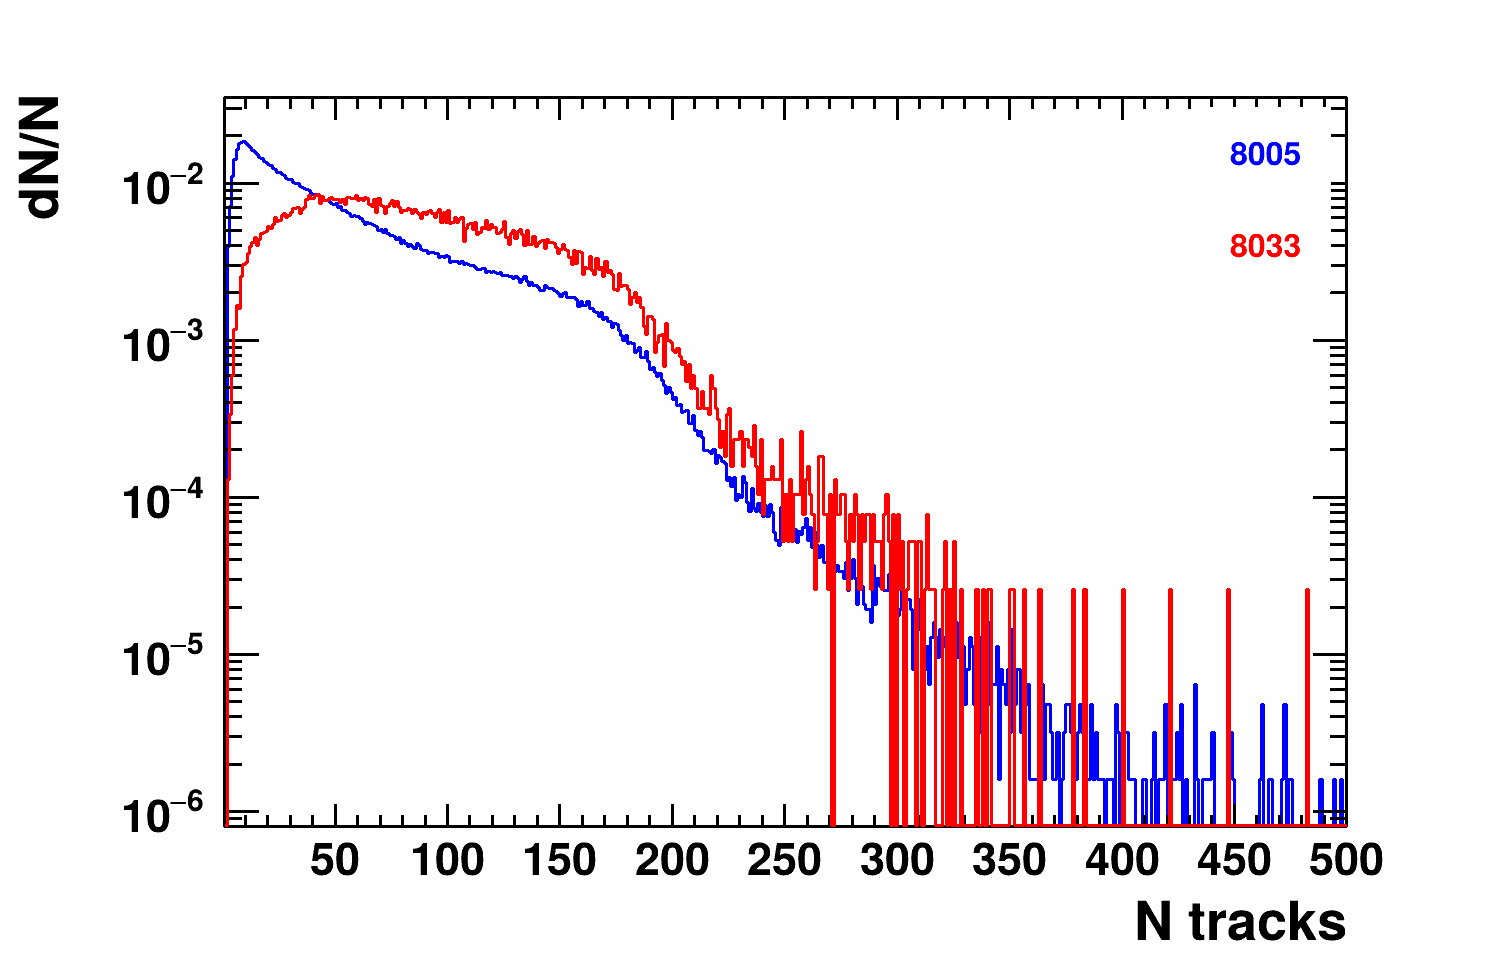
\includegraphics[width=0.35\linewidth]{../pict/QA_RunByRun_24.12/H1/nVtxTr_h2_RunId_nTracks.png}
            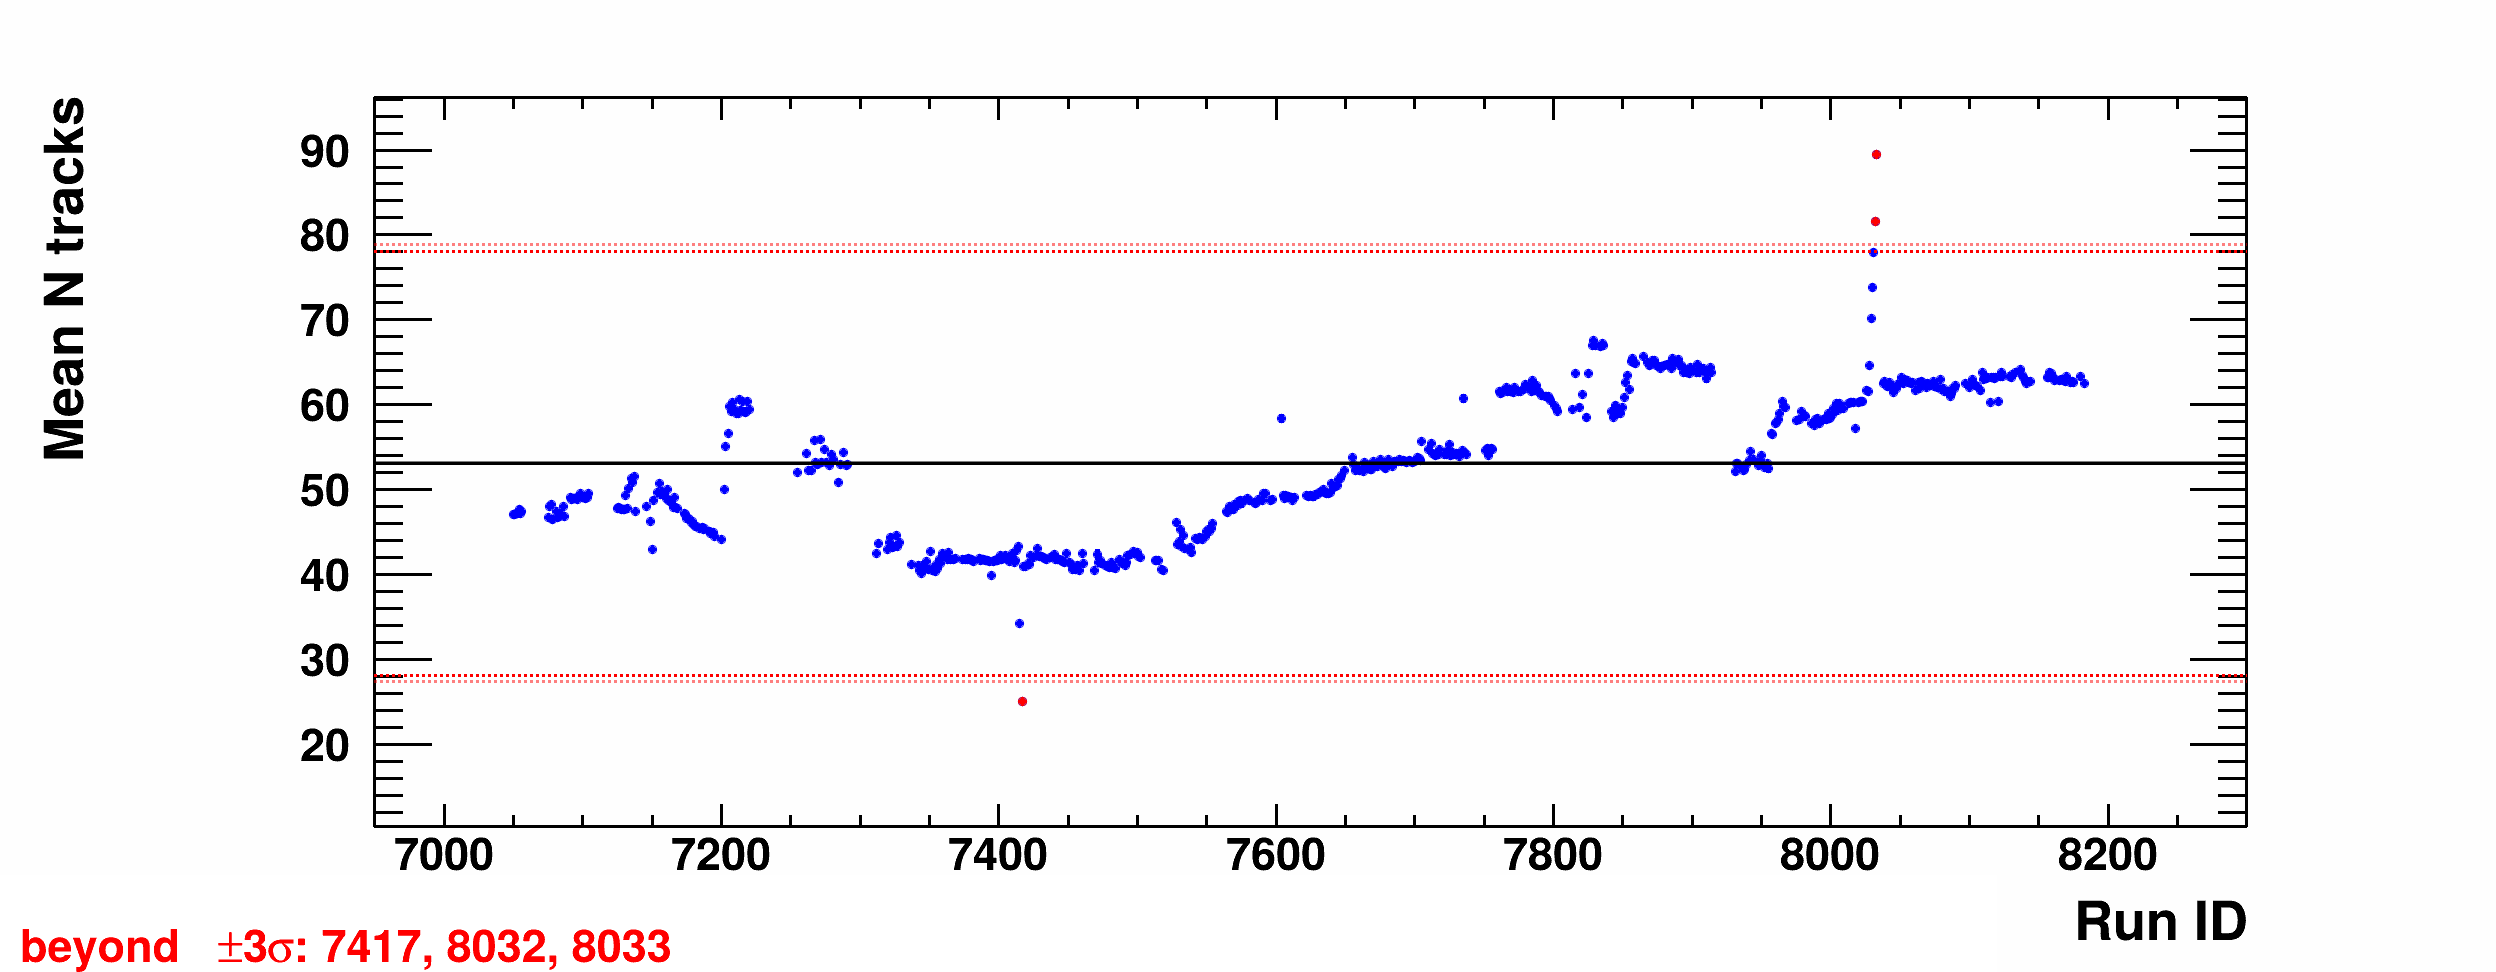
\includegraphics[width=0.60\linewidth]{../pict/QA_RunByRun_24.12/nVtxTr_h2_RunId_nTracks.png}
            \vspace{-3mm}
            \caption{Left panel: distribution of the number of charged particle in the tracking system (FSD + GEM). The red marker corresponds to the distribution from the "outlier" RunId. Right panel: Mean multiplicity as a function RunID. Black dotted horizontal line and red horizontal lines represent $\mu$ and $\pm3\sigma$, respectively.}
            \label{fig:mult}
        \end{center}
        \vspace{-5mm}
    \end{figure}




\subsection{Beam scintillation counters (BC)}

    Figure ~\ref{fig:BC1} shows the RunId dependence of the mean amplitude and integral of the summed signal in the beam scintillation counters (BC1). 
    Figure ~\ref{fig:BC2} shows a similar distribution for BC2 (in progress).

    %============================= Fig ================================
    \begin{figure}[H]
        \begin{center}
            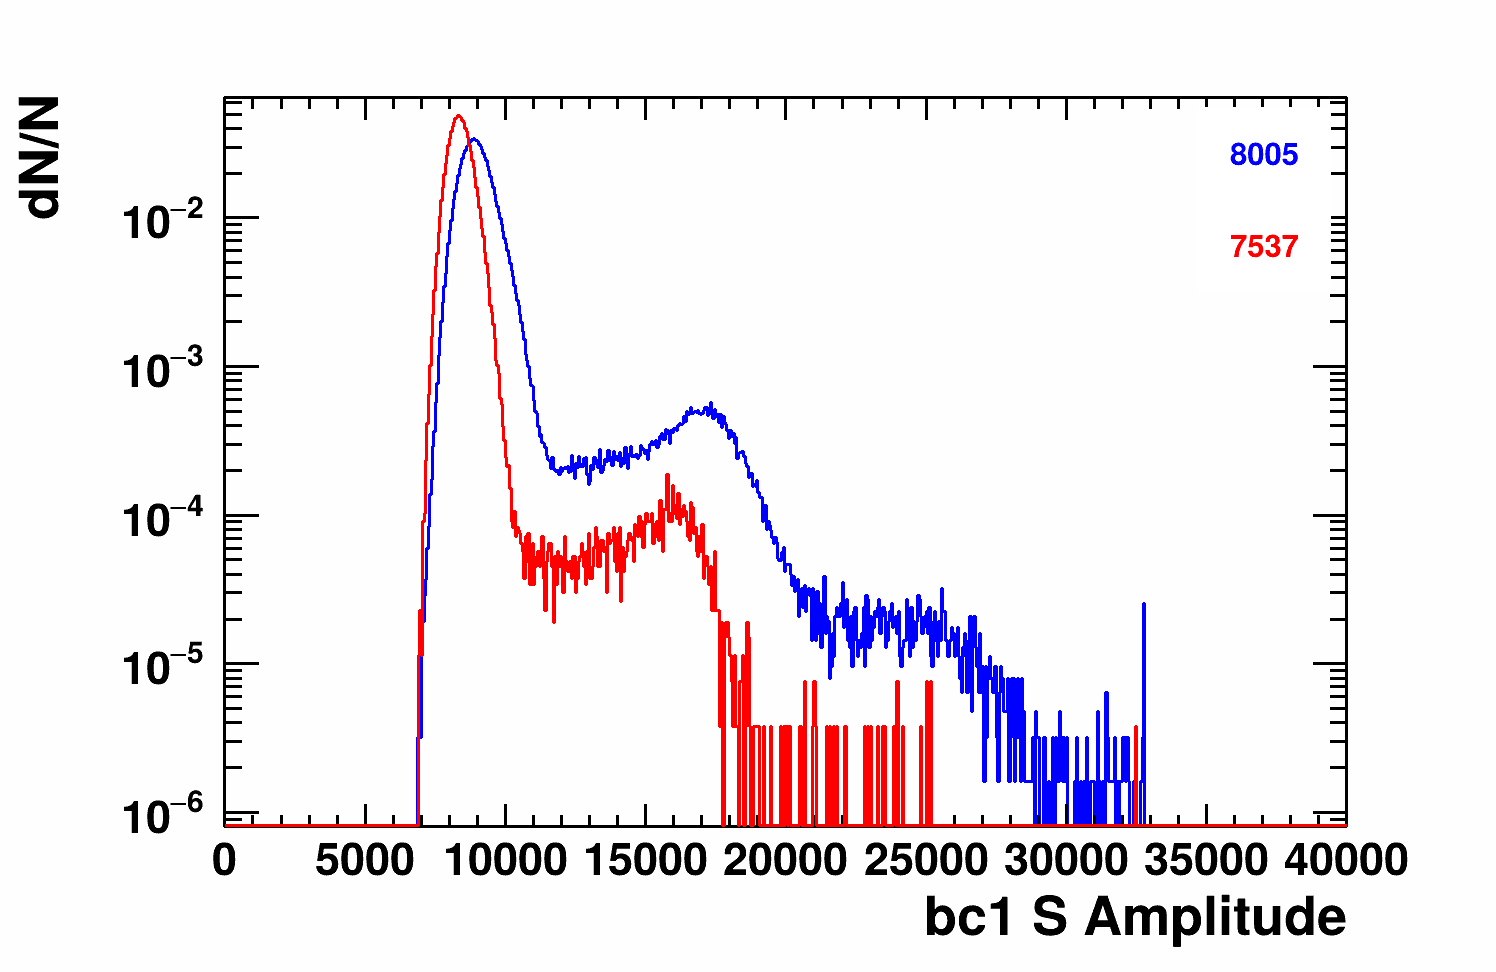
\includegraphics[width=0.35\linewidth]{../pict/QA_RunByRun_24.12/H1/nVtxTr_h2_RunId_bc1sAmp.png}
            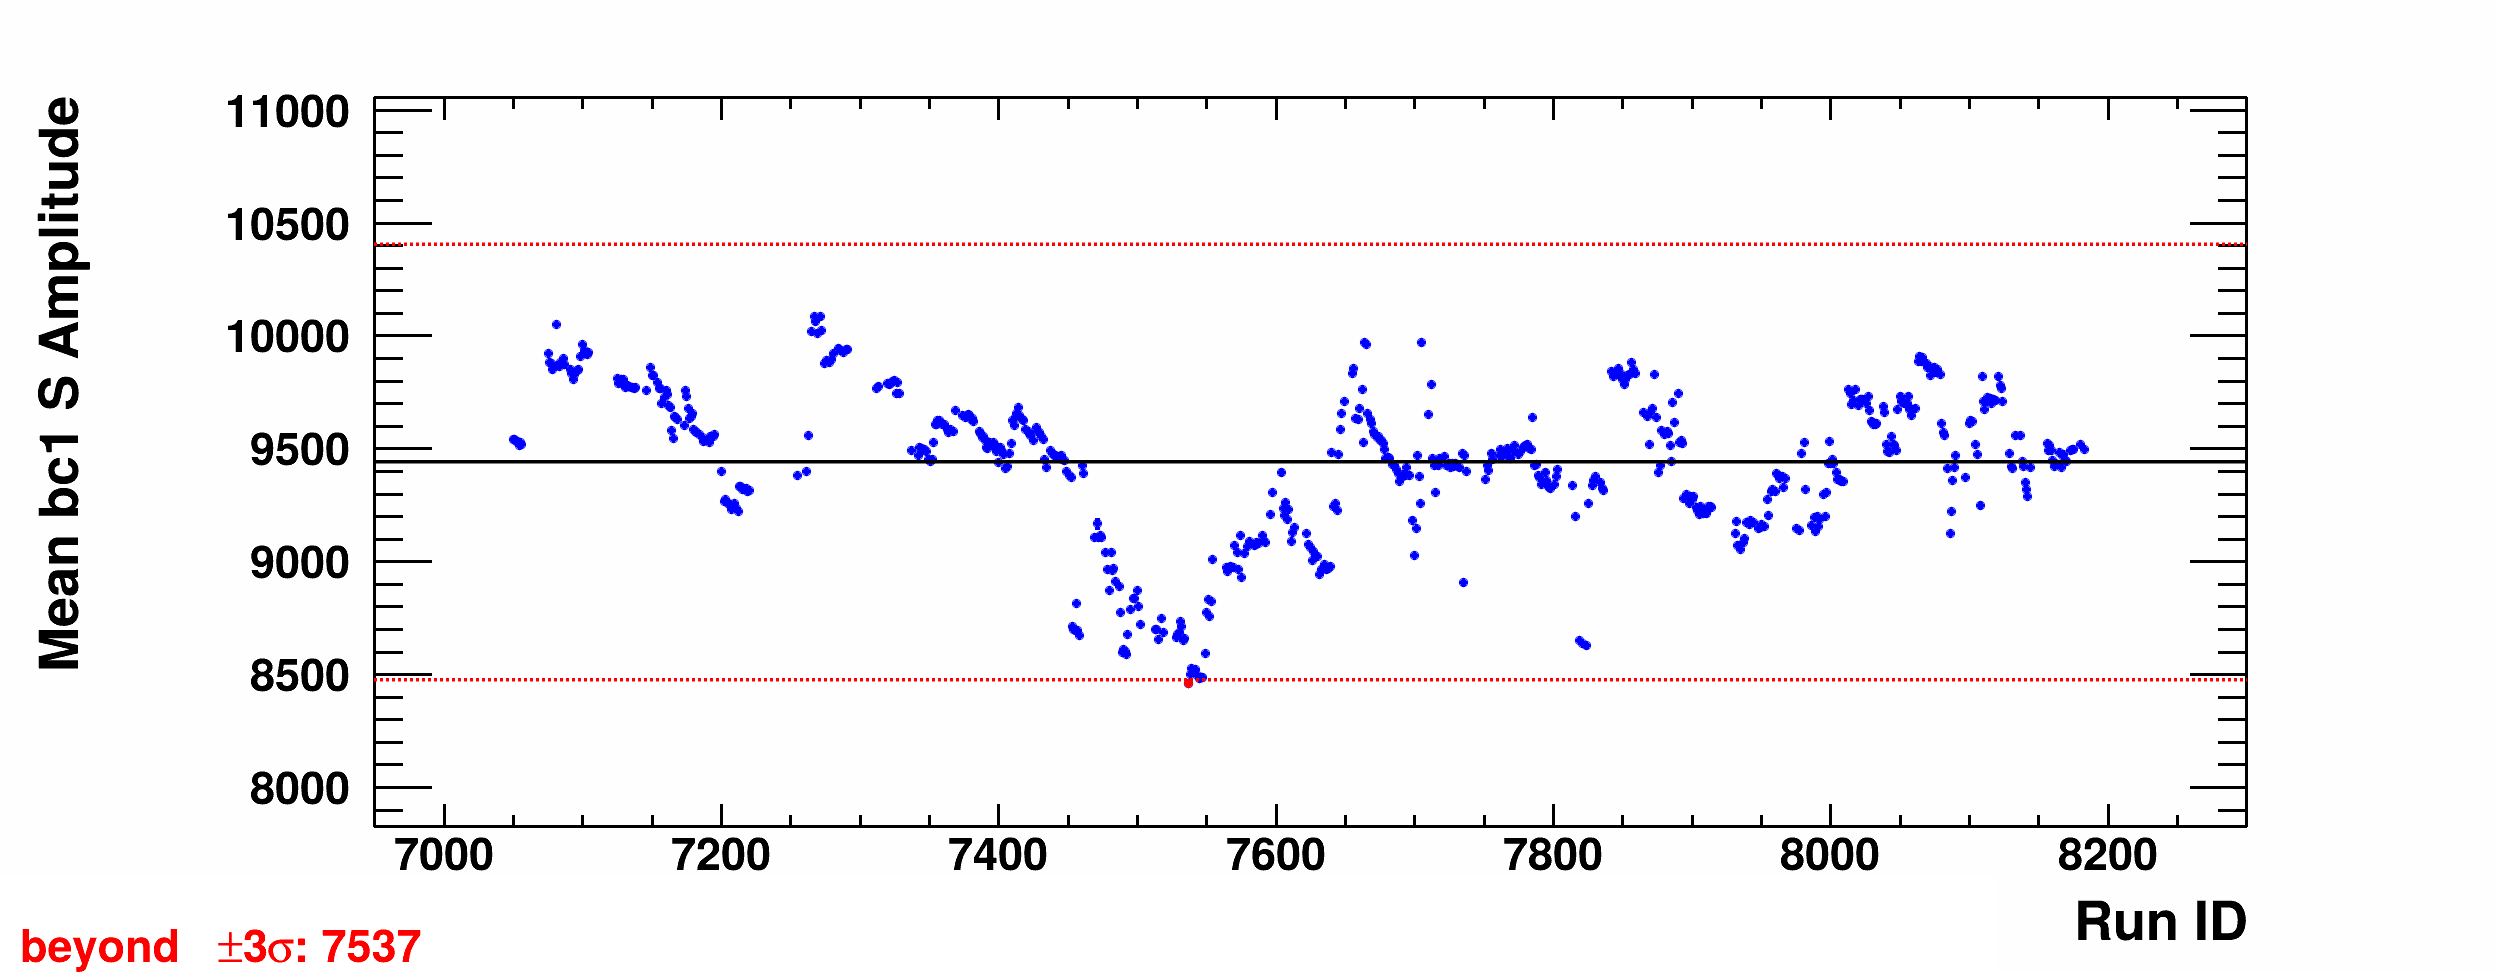
\includegraphics[width=0.60\linewidth]{../pict/QA_RunByRun_24.12/nVtxTr_h2_RunId_bc1sAmp.png}

            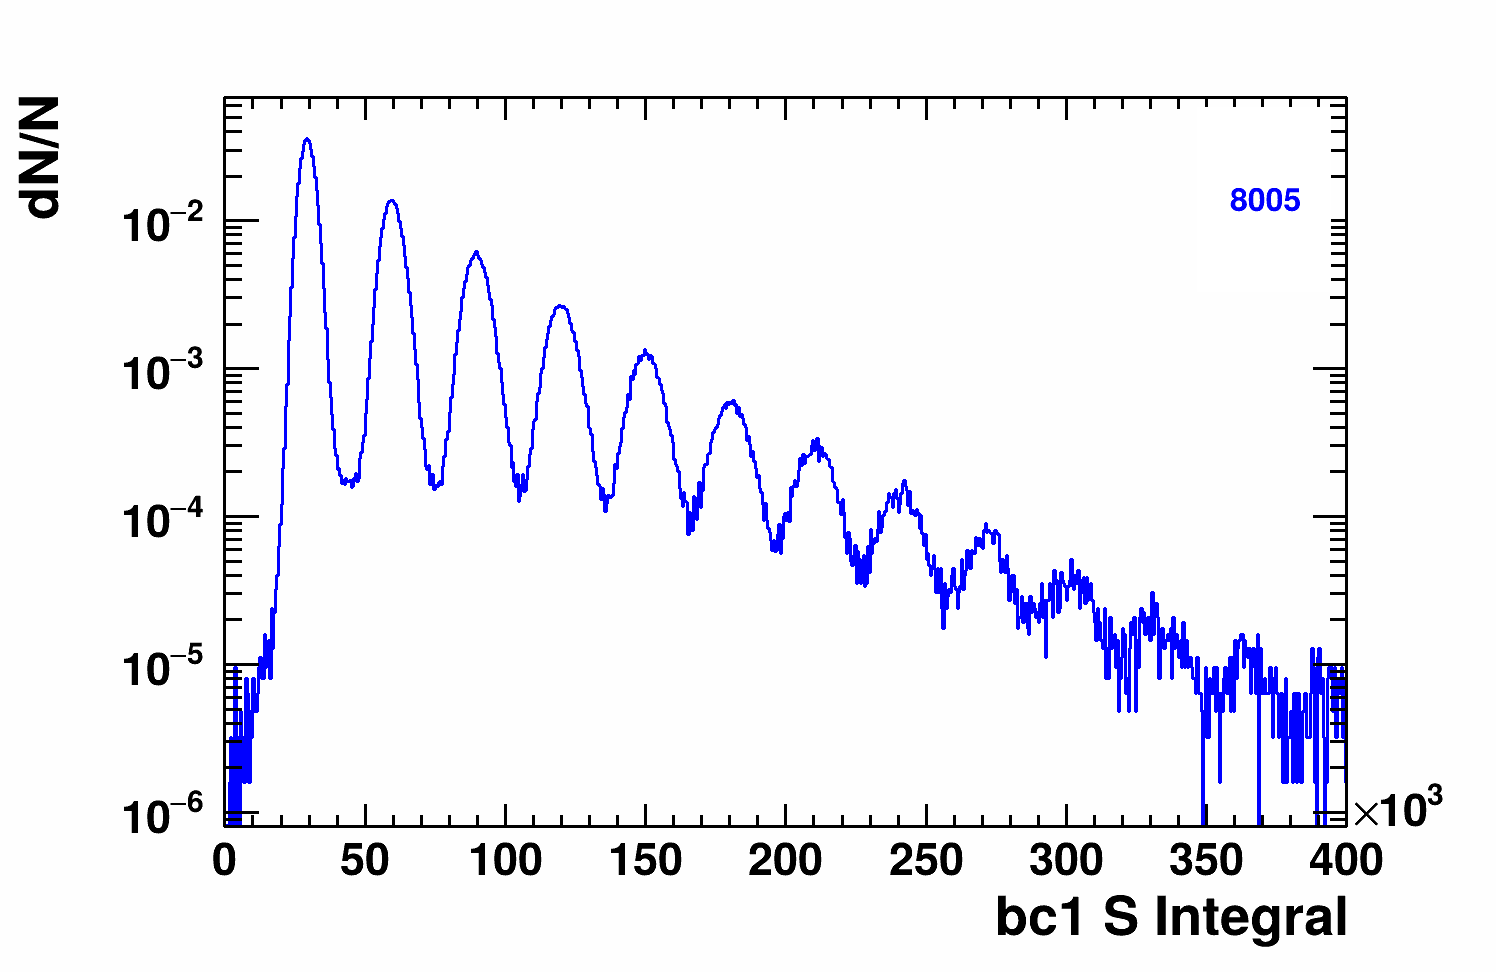
\includegraphics[width=0.35\linewidth]{../pict/QA_RunByRun_24.12/H1/nVtxTr_h2_RunId_bc1sInt.png}
            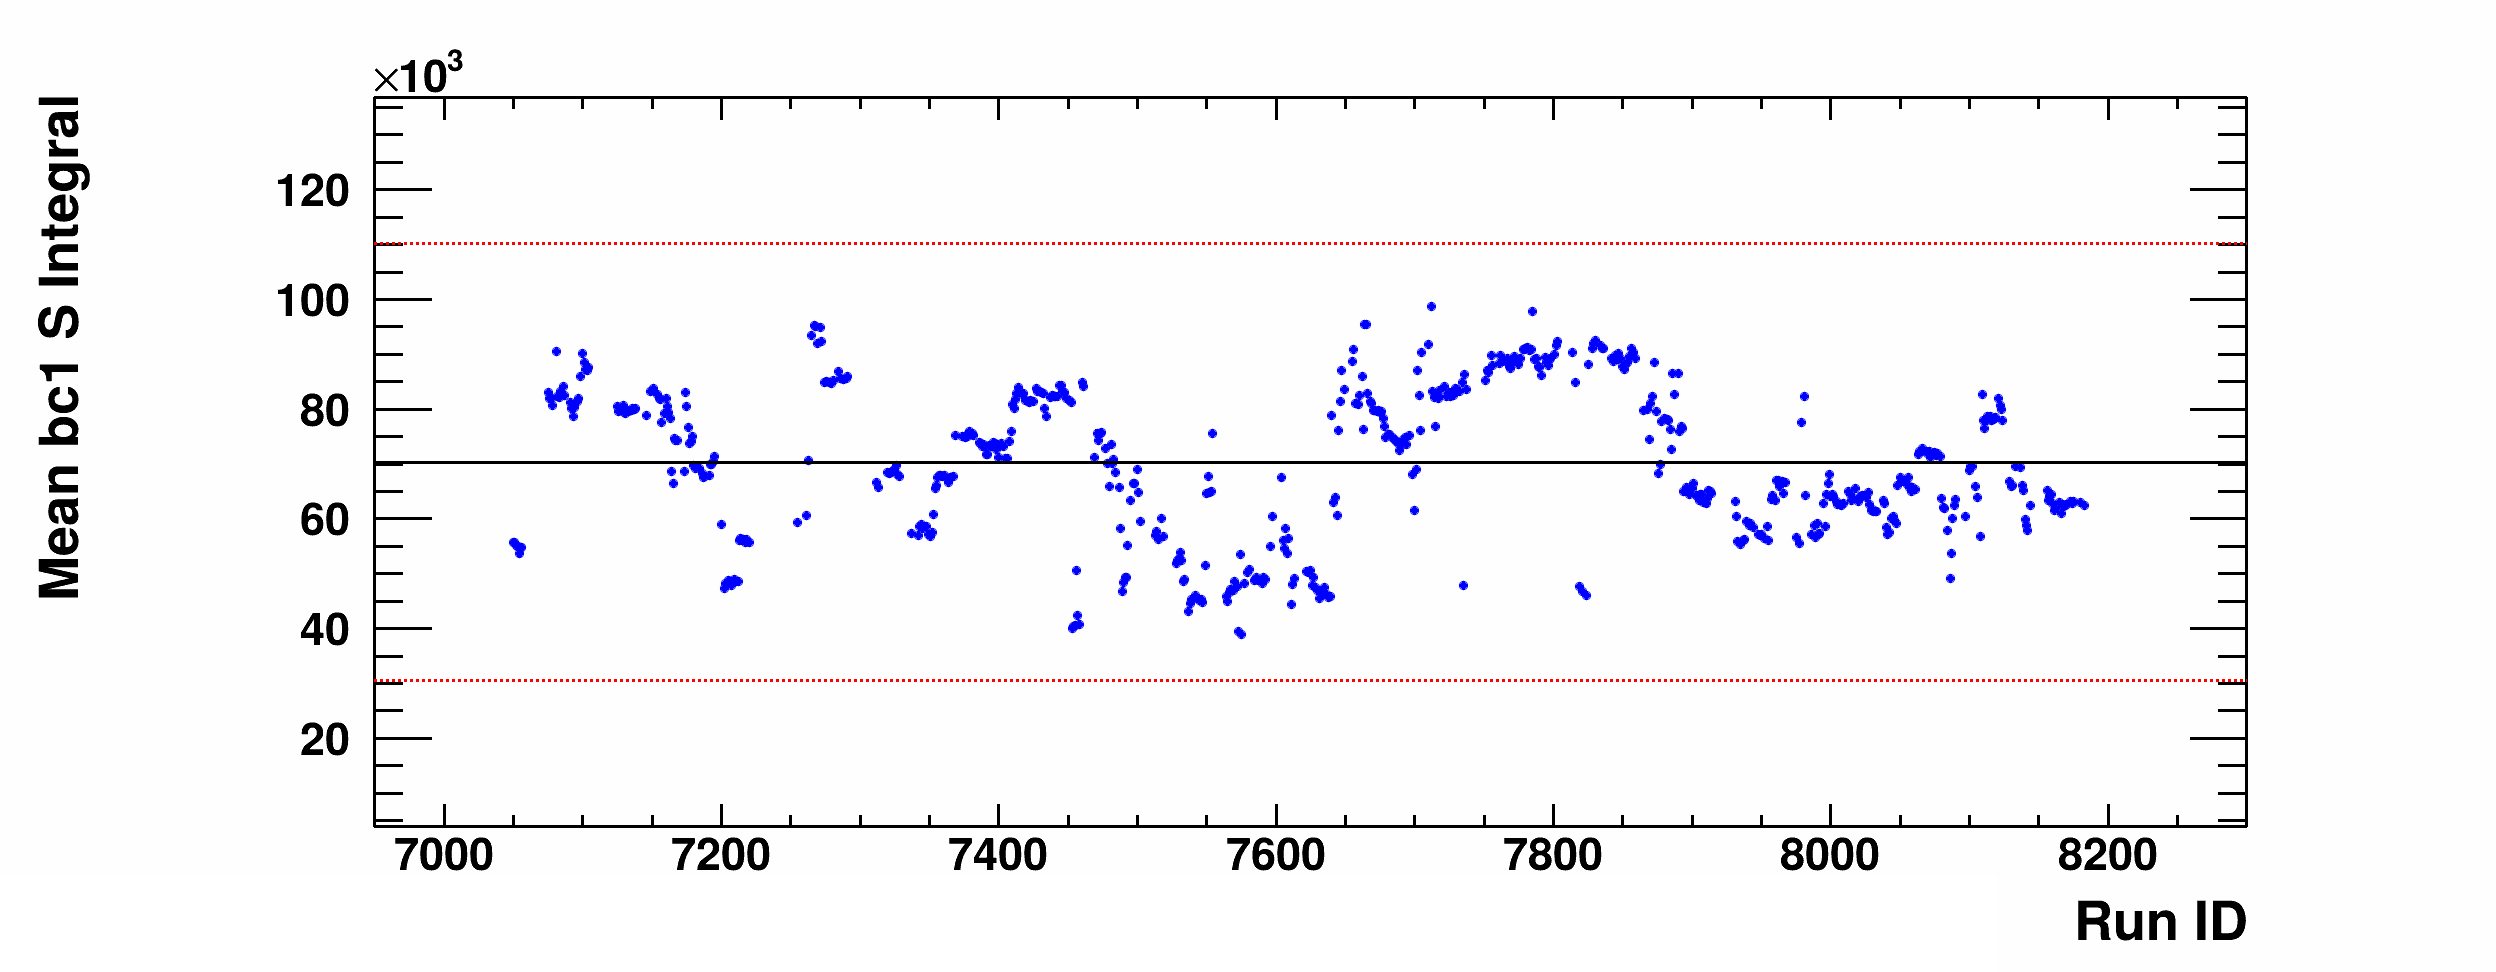
\includegraphics[width=0.60\linewidth]{../pict/QA_RunByRun_24.12/nVtxTr_h2_RunId_bc1sInt.png}
            \vspace{-3mm}
            \caption{Left panels: Distribution of the amplitude and integral of the summed signal in the BC1. The red marker corresponds to the distribution from the "outlier" RunId. Right panels: Mean amplitude and integral as a function RunID. Black dotted horizontal line and red horizontal lines represent $\mu$ and $\pm3\sigma$, respectively.}
            \label{fig:BC1}
        \end{center}
        \vspace{-5mm}
    \end{figure}

    %============================= Fig ================================
    \begin{figure}[H]
        \begin{center}
            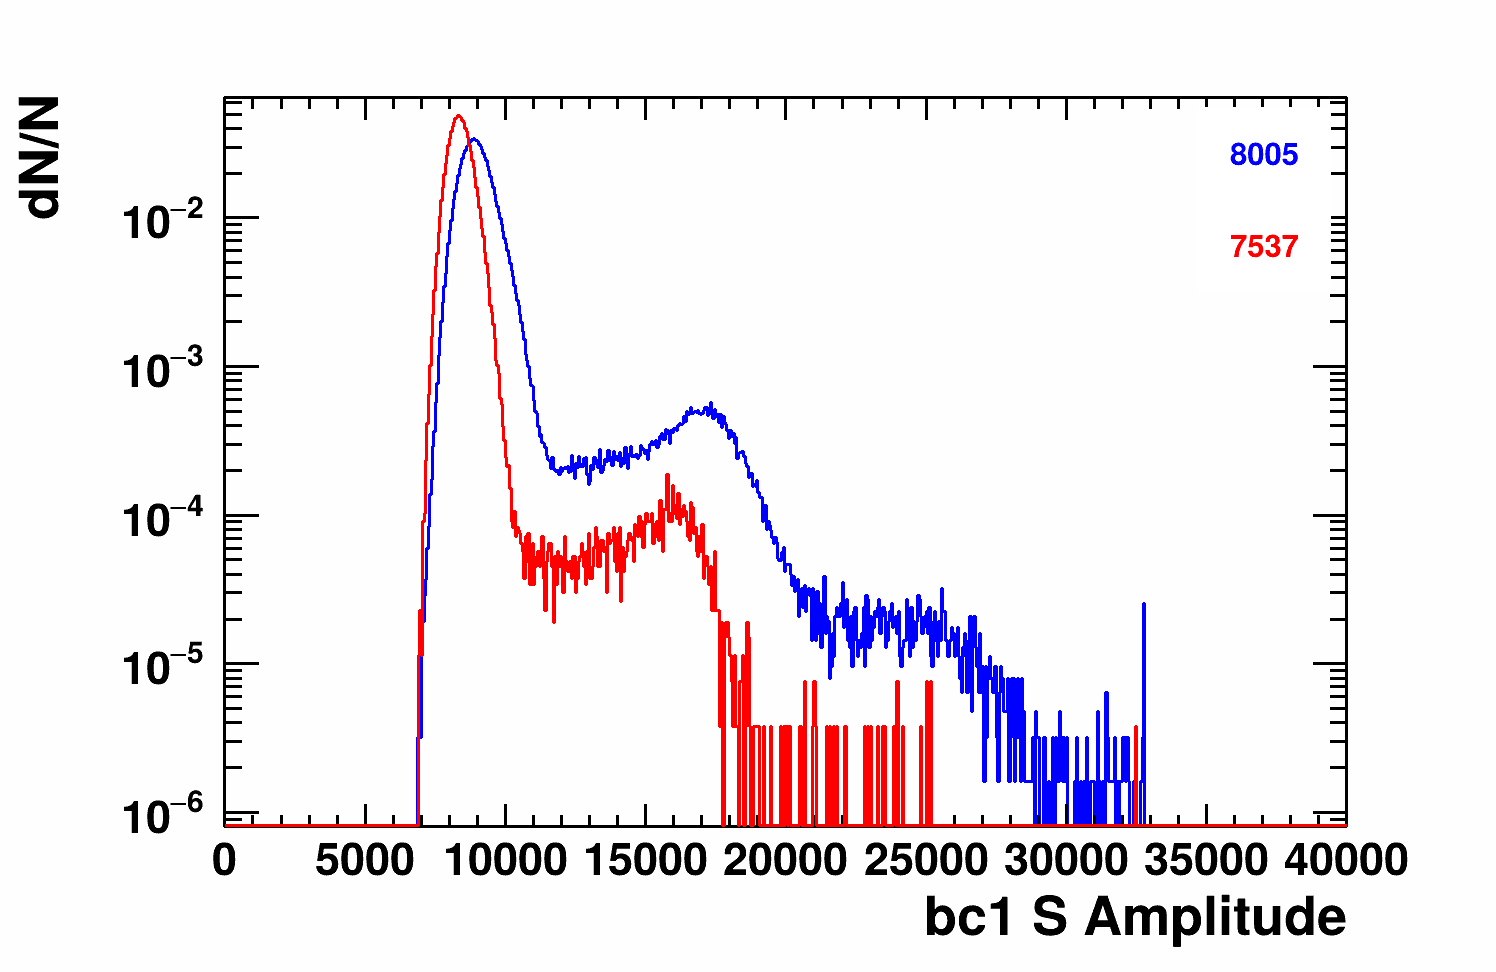
\includegraphics[width=0.35\linewidth]{../pict/QA_RunByRun_24.12/H1/nVtxTr_h2_RunId_bc1sAmp.png}
            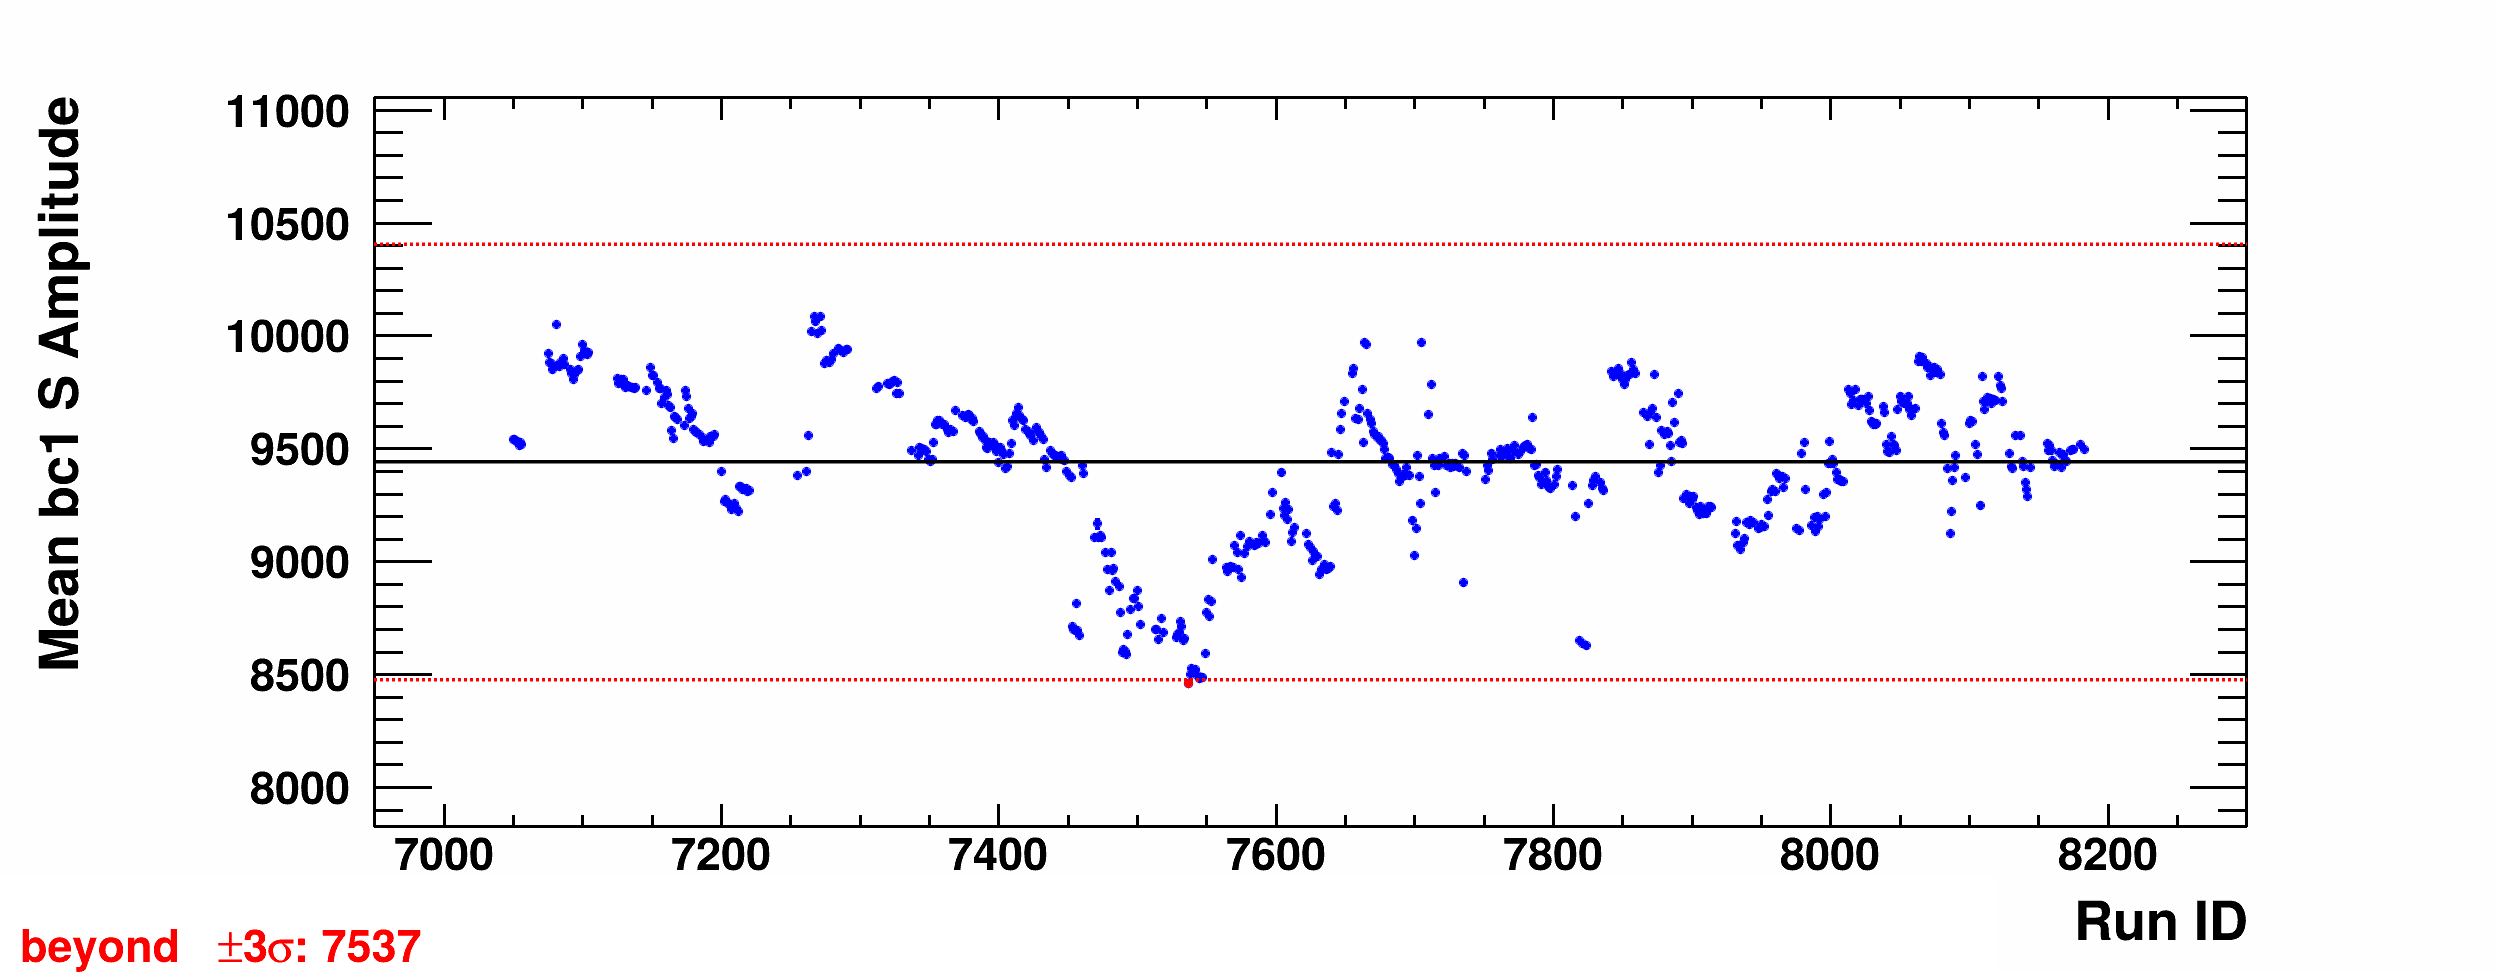
\includegraphics[width=0.60\linewidth]{../pict/QA_RunByRun_24.12/nVtxTr_h2_RunId_bc1sAmp.png}

            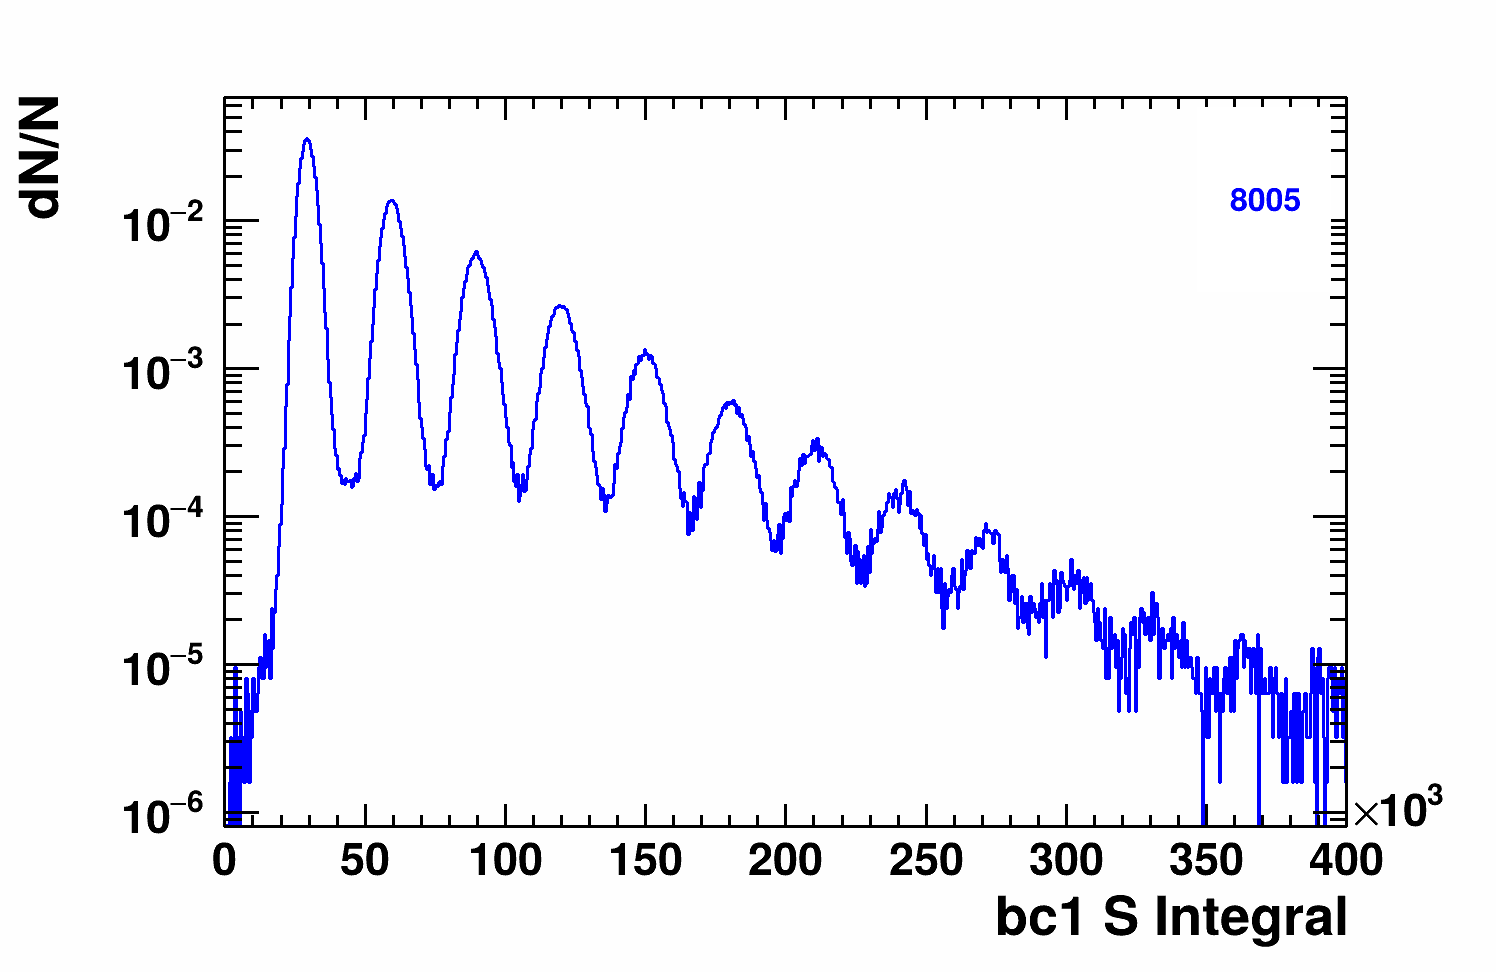
\includegraphics[width=0.35\linewidth]{../pict/QA_RunByRun_24.12/H1/nVtxTr_h2_RunId_bc1sInt.png}
            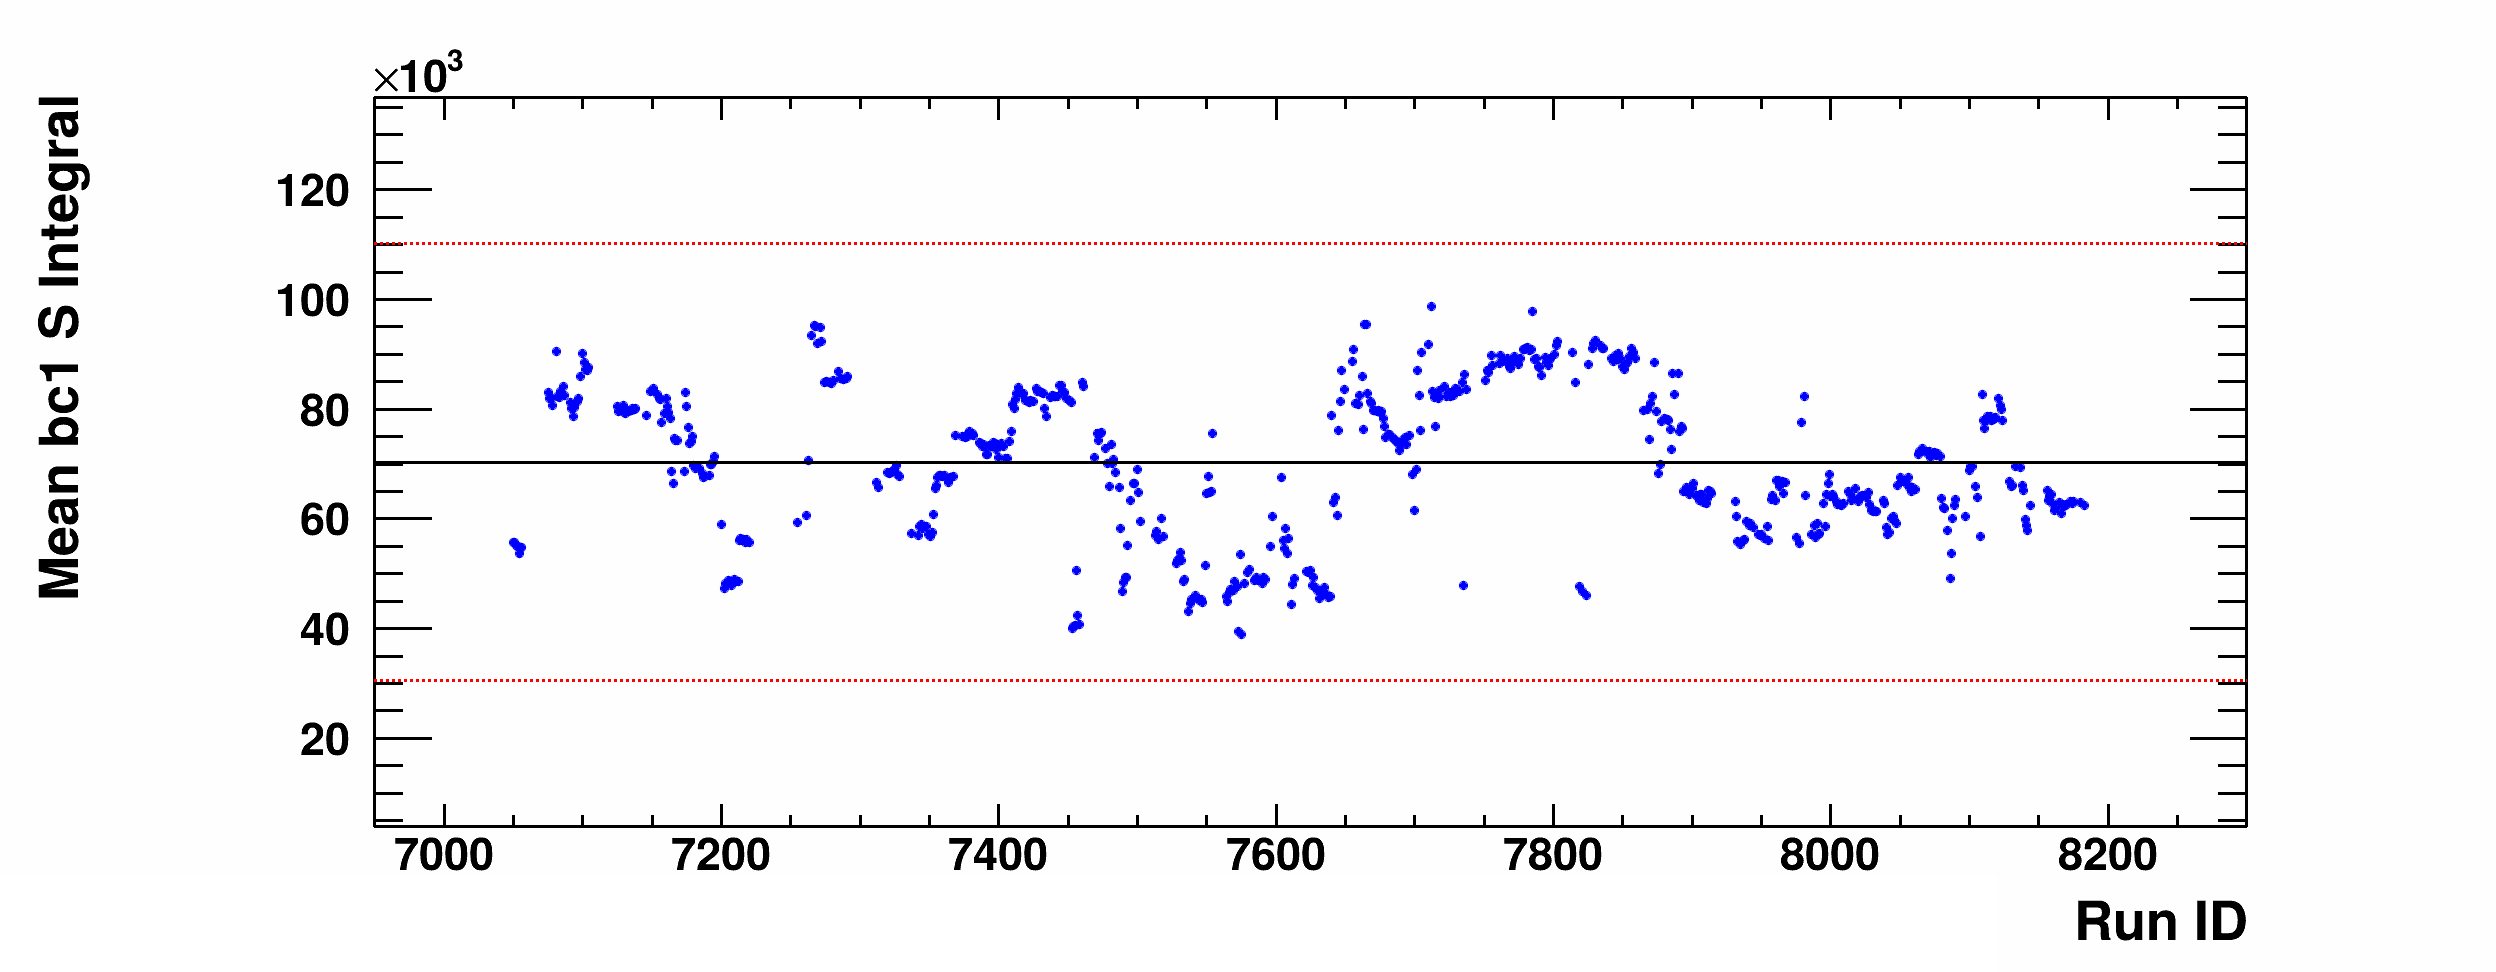
\includegraphics[width=0.60\linewidth]{../pict/QA_RunByRun_24.12/nVtxTr_h2_RunId_bc1sInt.png}
            \vspace{-3mm}
            \caption{Left panels: Distribution of the amplitude and integral of the summed signal in the BC2. The red marker corresponds to the distribution from the "outlier" RunId. Right panels: Mean amplitude and integral as a function RunID. Black dotted horizontal line and red horizontal lines represent $\mu$ and $\pm3\sigma$, respectively.}
            \label{fig:BC2}
        \end{center}
        \vspace{-5mm}
    \end{figure}




\subsection{Scintillation Veto counter (VC)}

    Figure ~\ref{fig:VC} shows he RunId dependence of the mean amplitude and integral of the summed signal in the scintillation Veto counter (VC).    

    %============================= Fig ================================
    \begin{figure}[H]
        \begin{center}
            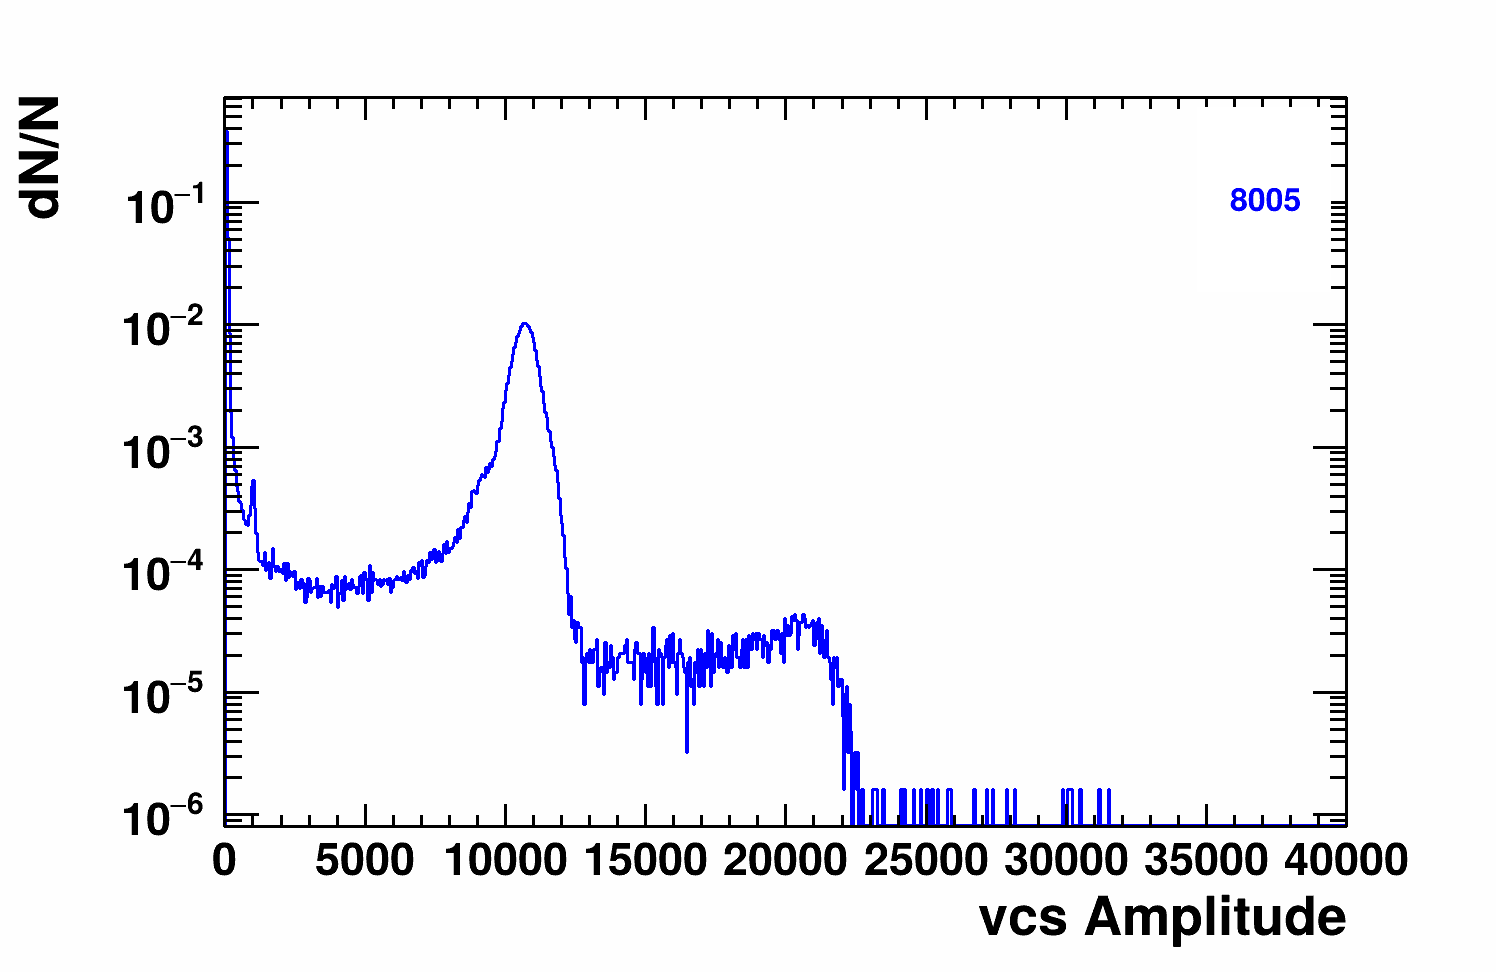
\includegraphics[width=0.35\linewidth]{../pict/QA_RunByRun_24.12/H1/nVtxTr_h2_RunId_vcsAmp.png}
            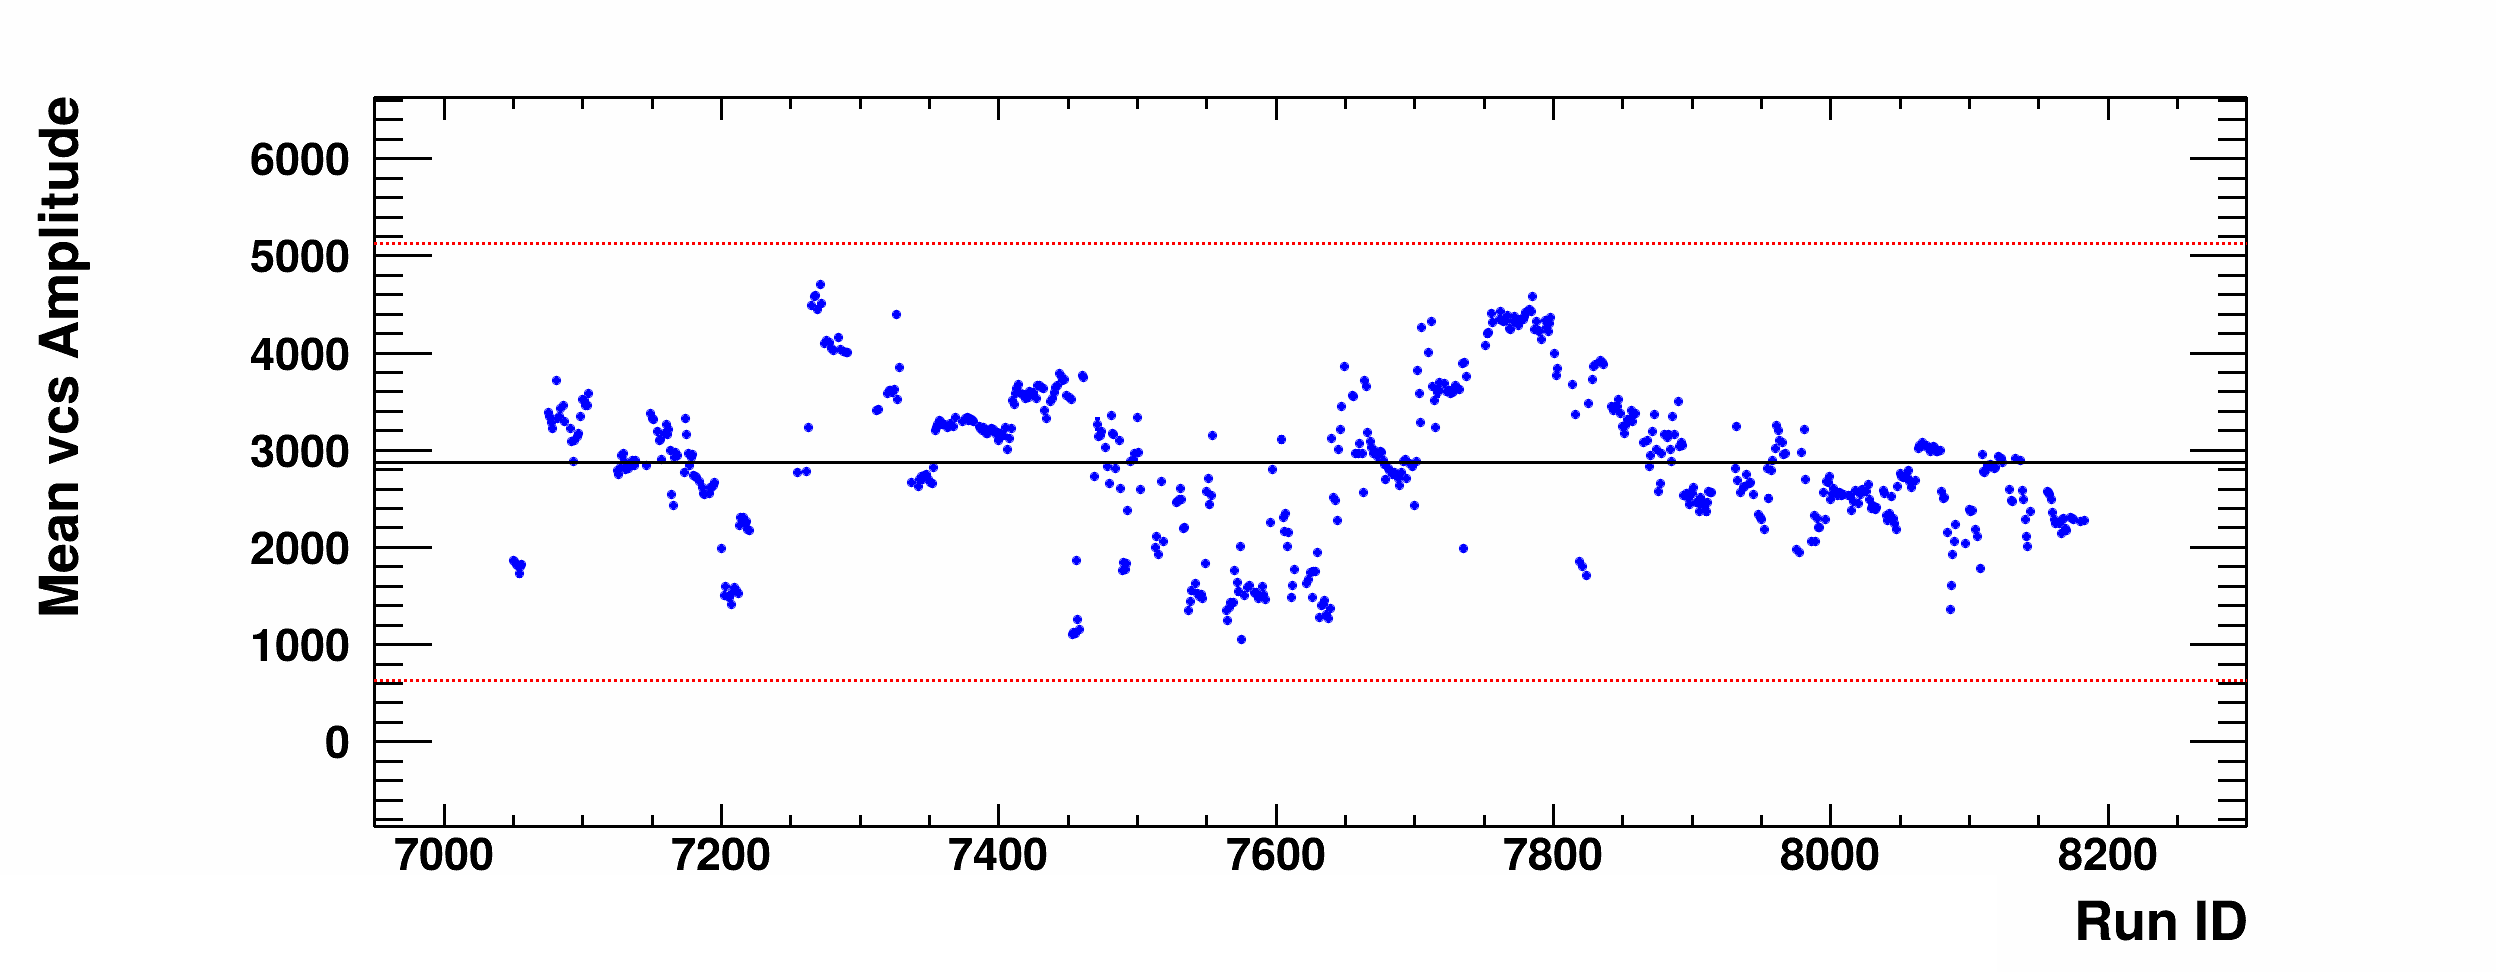
\includegraphics[width=0.60\linewidth]{../pict/QA_RunByRun_24.12/nVtxTr_h2_RunId_vcsAmp.png}

            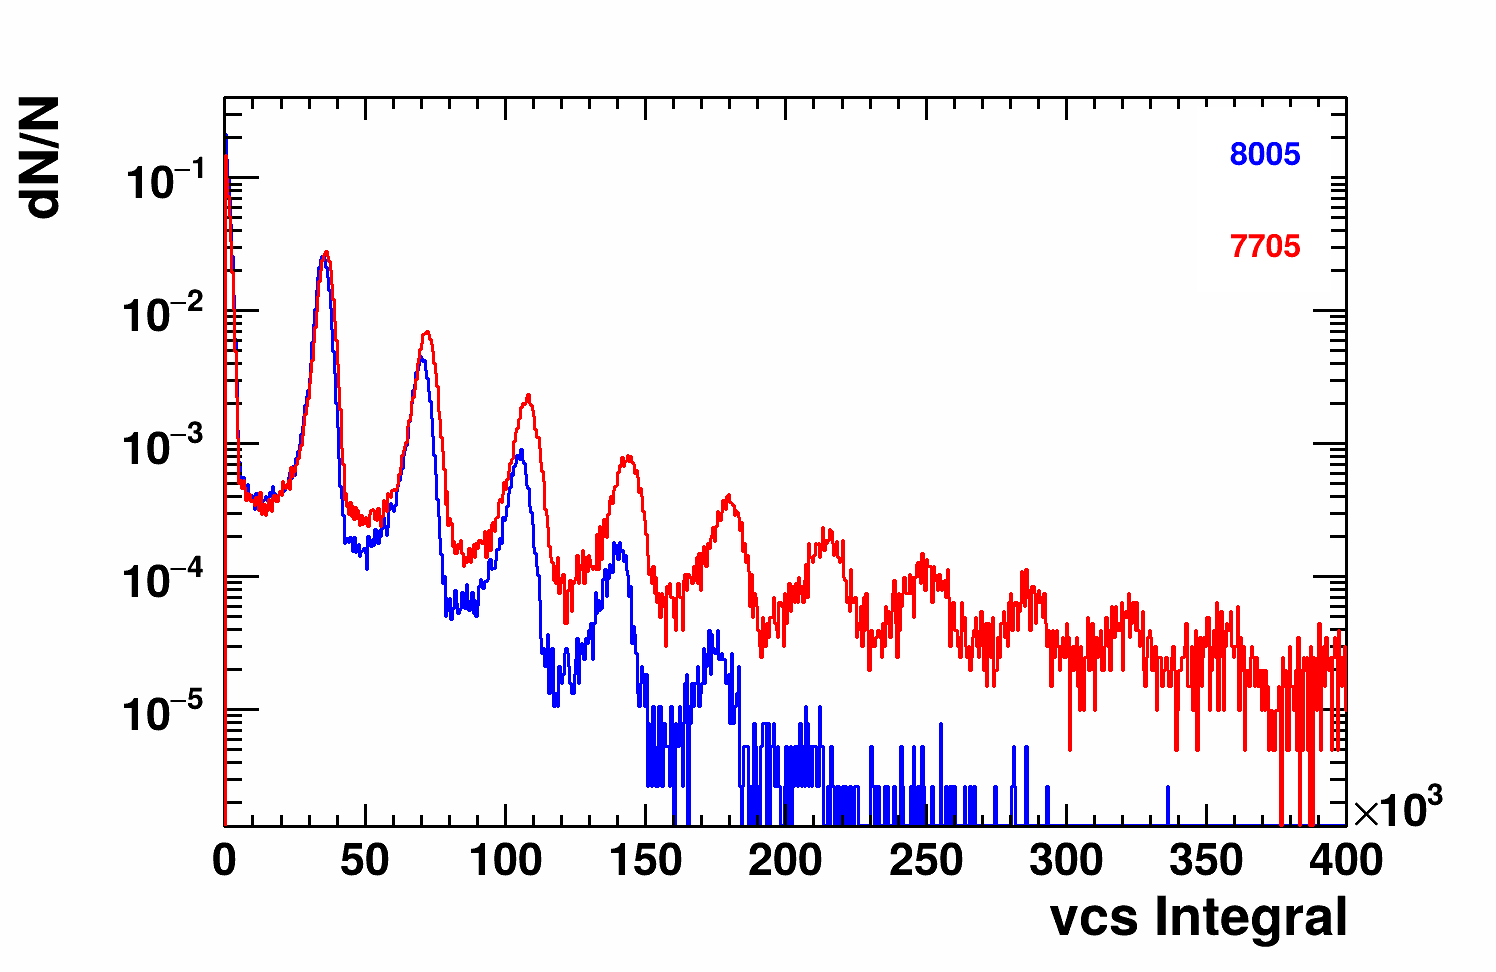
\includegraphics[width=0.35\linewidth]{../pict/QA_RunByRun_24.12/H1/nVtxTr_h2_RunId_vcsInt.png}
            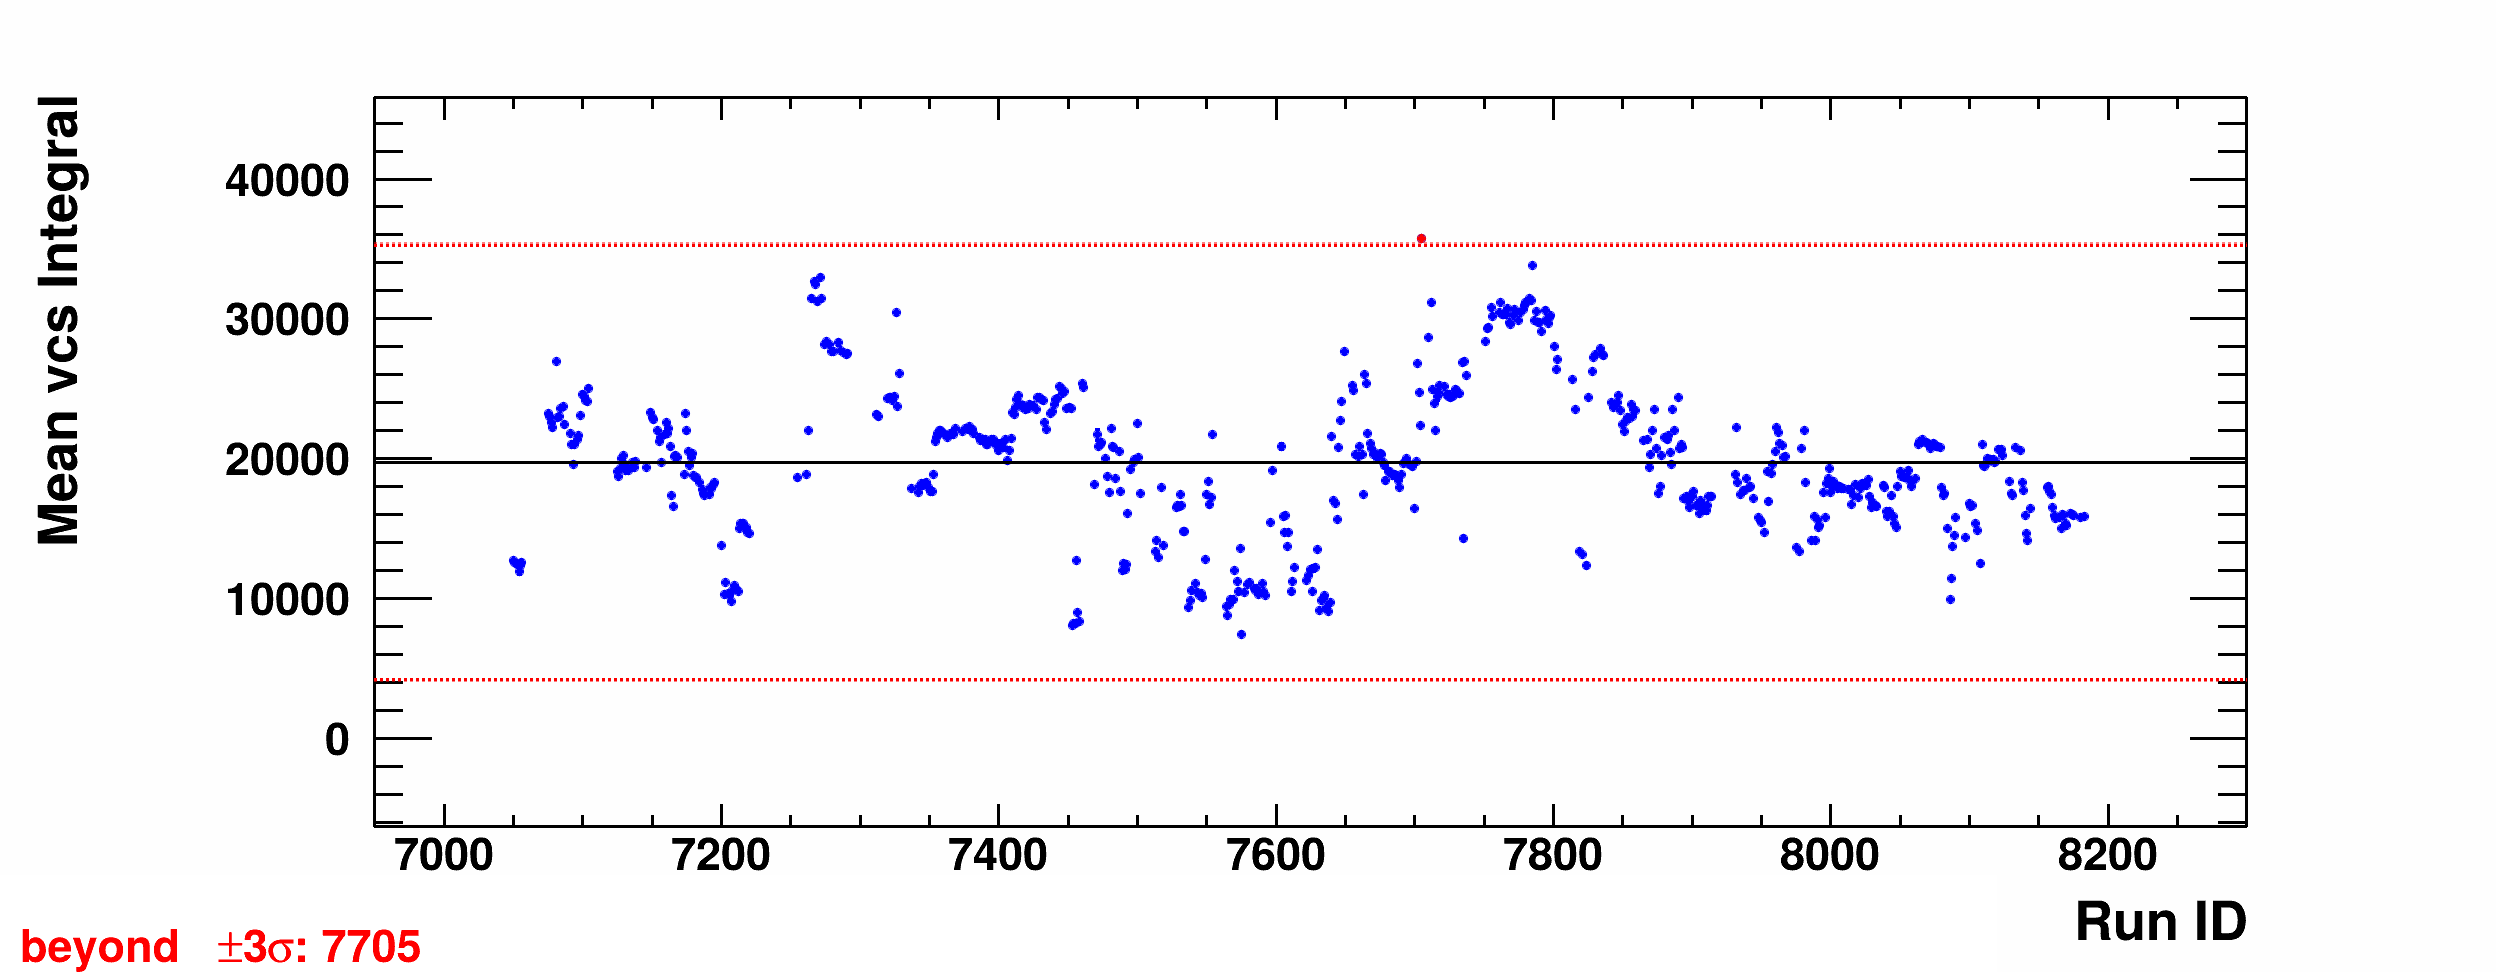
\includegraphics[width=0.60\linewidth]{../pict/QA_RunByRun_24.12/nVtxTr_h2_RunId_vcsInt.png}
            \vspace{-3mm}
            \caption{Left panels: Distribution of the amplitude and integral of the summed signal in the VC. The red marker corresponds to the distribution from the "outlier" RunId. Right panels: Mean amplitude and integral as a function RunID. Black dotted horizontal line and red horizontal lines represent $\mu$ and $\pm3\sigma$, respectively.}
            \label{fig:VC}
        \end{center}
        \vspace{-5mm}
    \end{figure}




\subsection{Fragment Detector (FD)}

    Figure ~\ref{fig:FD} shows he RunId dependence of the mean amplitude and integral of signal in the fragment detector (FD). Figure ~\ref{fig:bc1_vs_fd} shows correlation between the integral of signal from FD and BC1. The figure ~\ref{fig:bc1_vs_fd} shows the correlation between the integral of the signal from FD and the integral of the summed signal from BC1.

    %============================= Fig ================================
    \begin{figure}[H]
        \begin{center}
            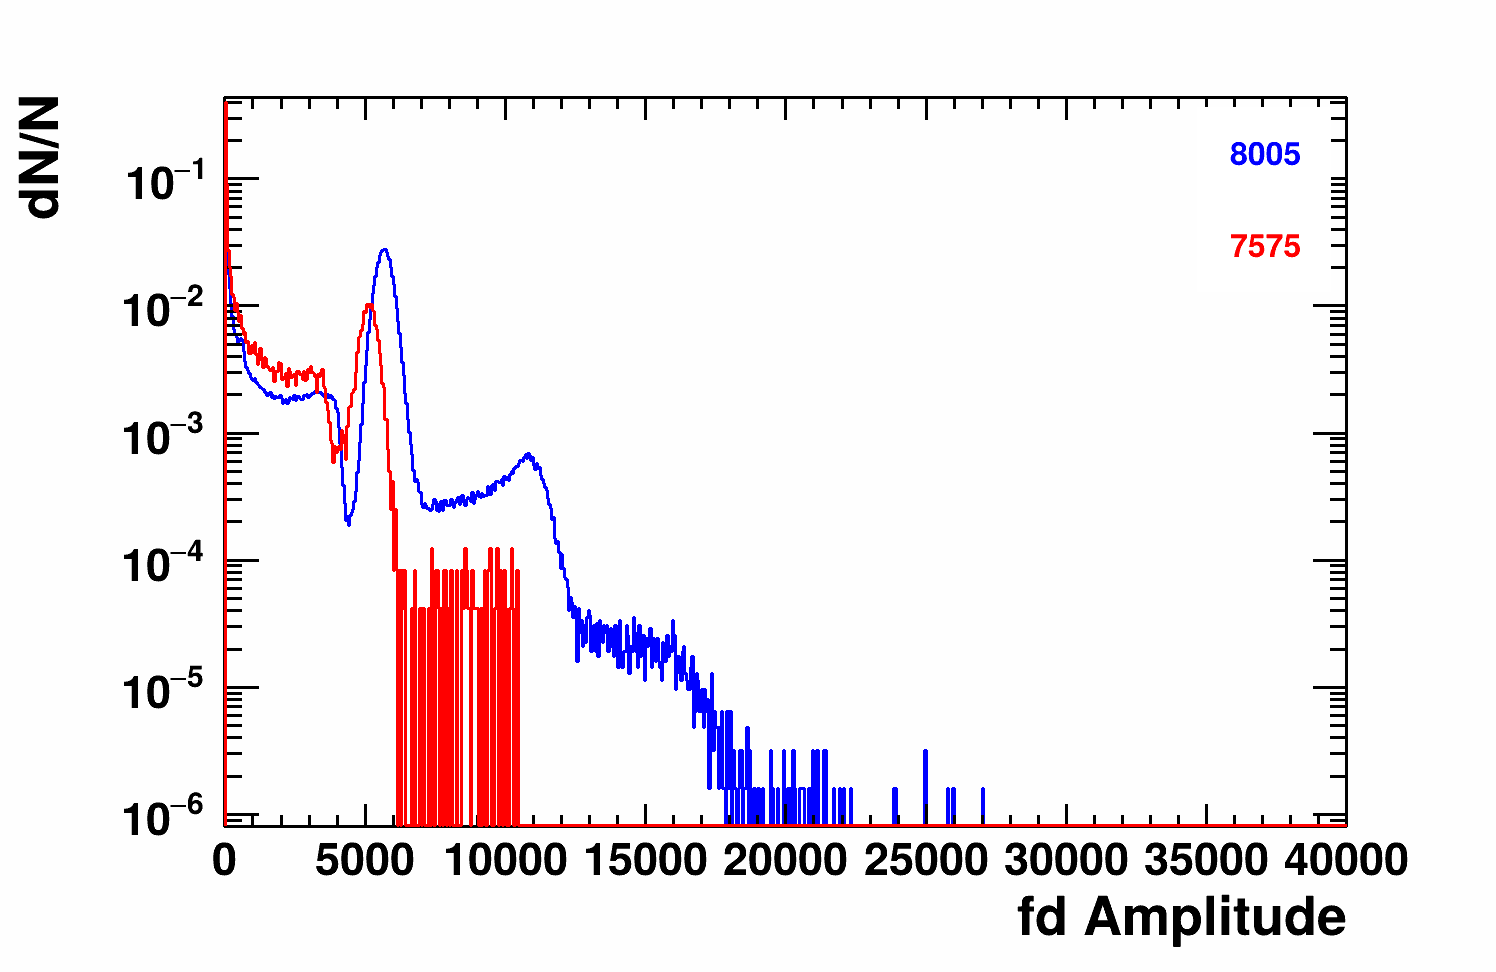
\includegraphics[width=0.35\linewidth]{../pict/QA_RunByRun_24.12/H1/nVtxTr_h2_RunId_fdAmp.png}
            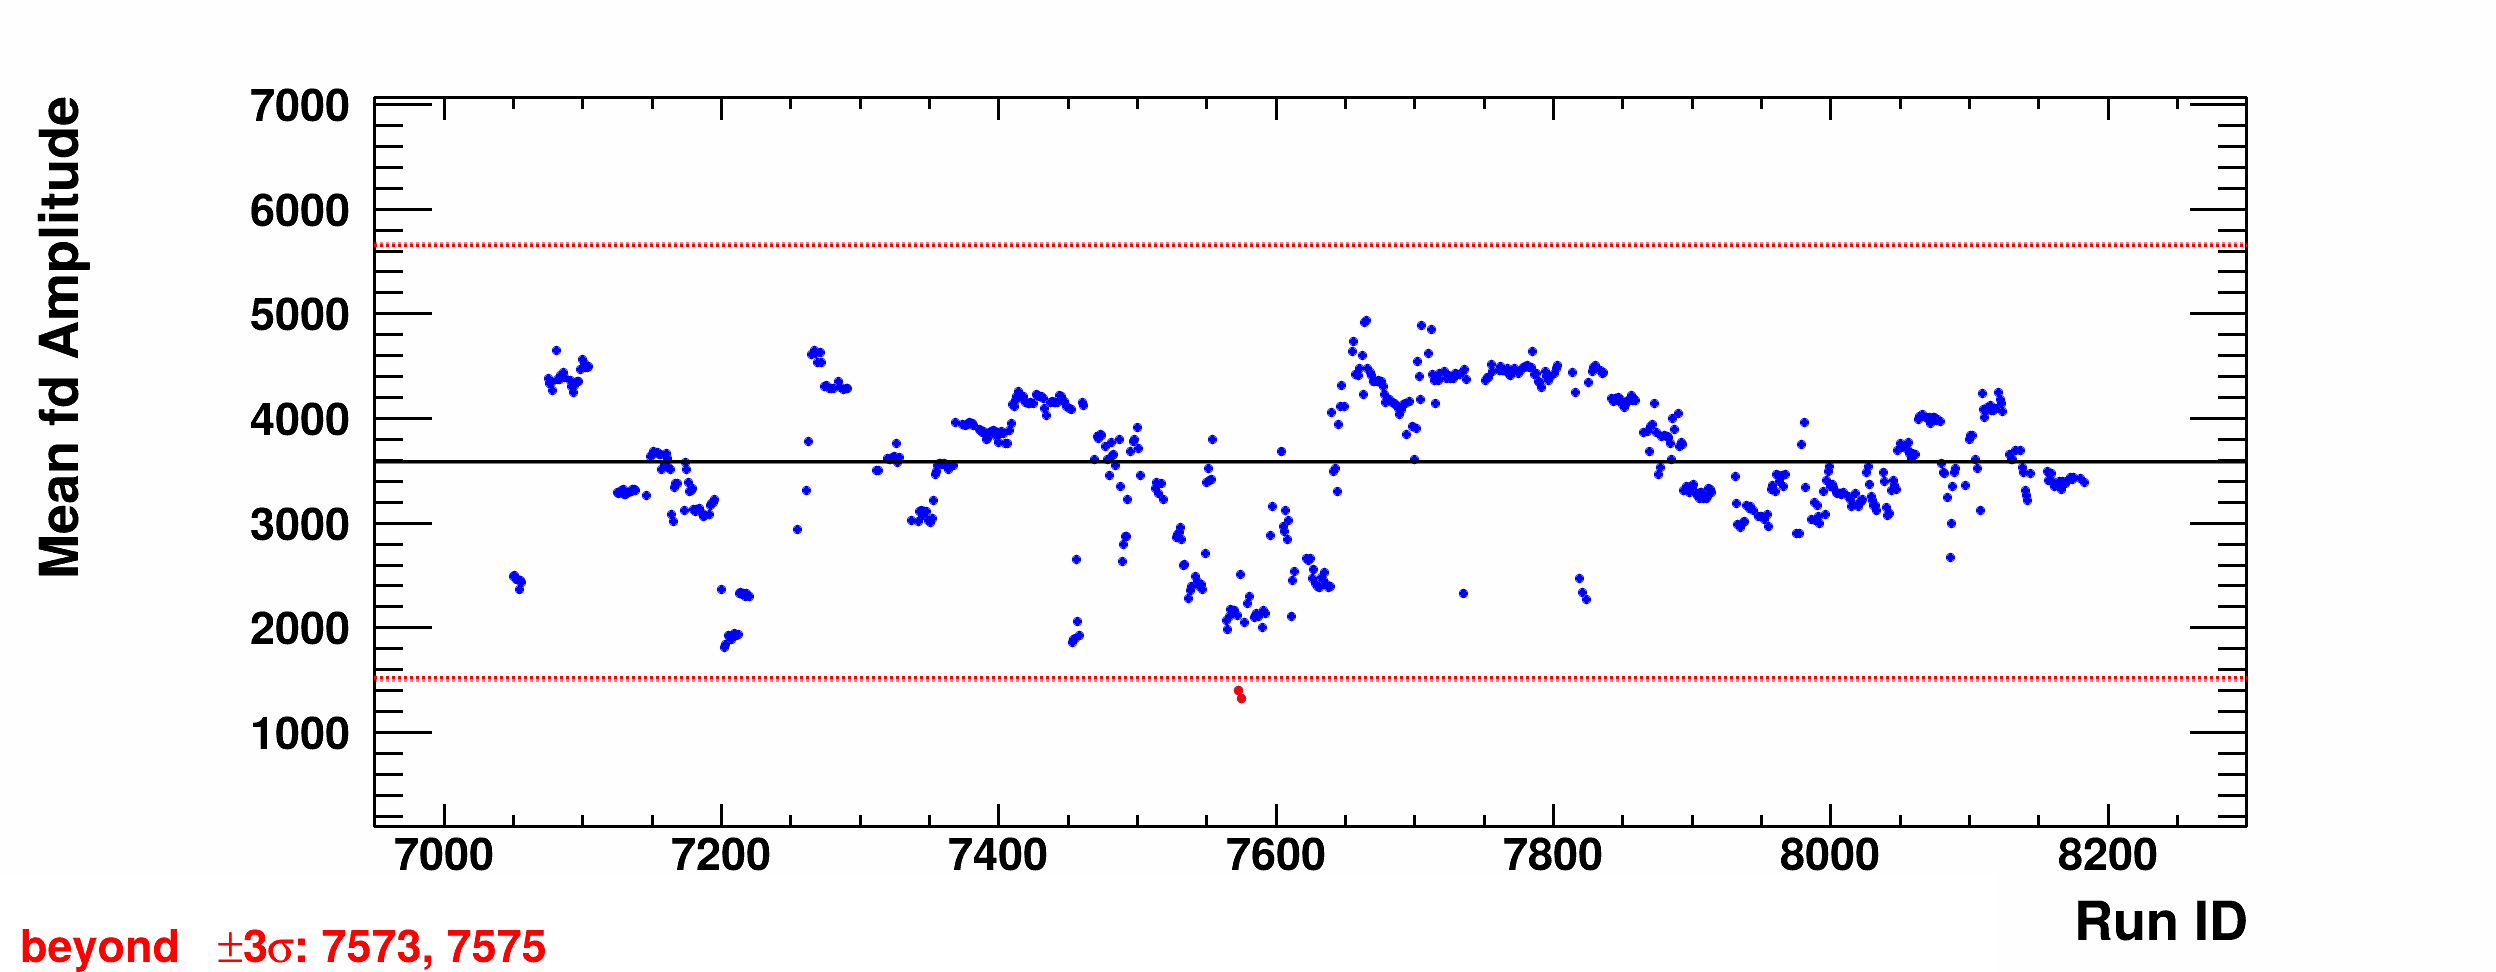
\includegraphics[width=0.60\linewidth]{../pict/QA_RunByRun_24.12/nVtxTr_h2_RunId_fdAmp.png}
            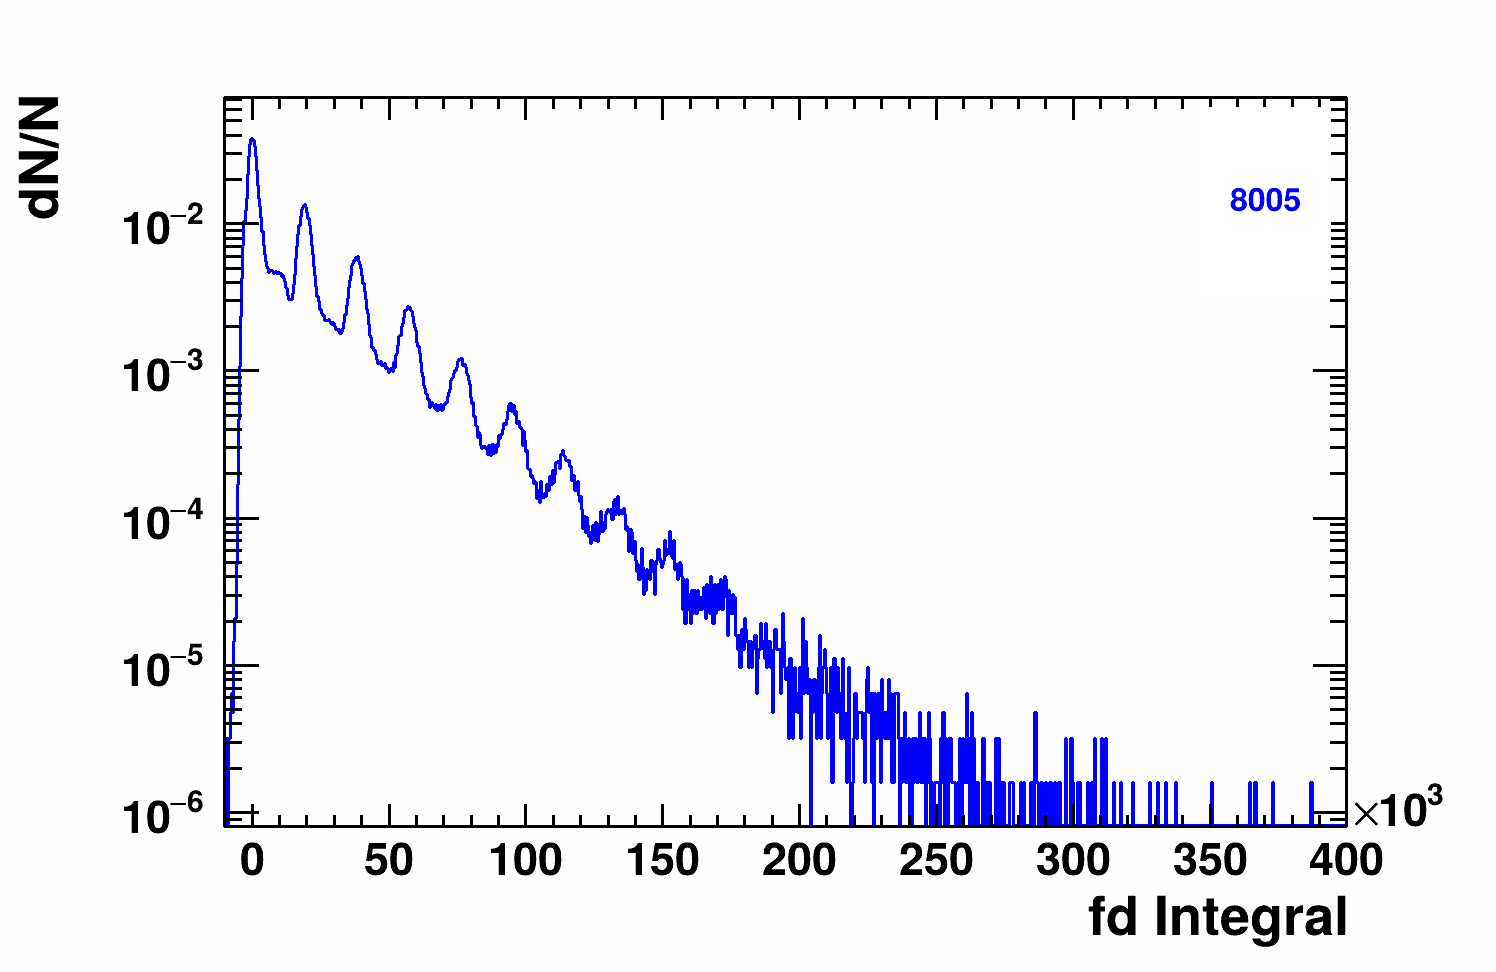
\includegraphics[width=0.35\linewidth]{../pict/QA_RunByRun_24.12/H1/nVtxTr_h2_RunId_fdInt.png}
            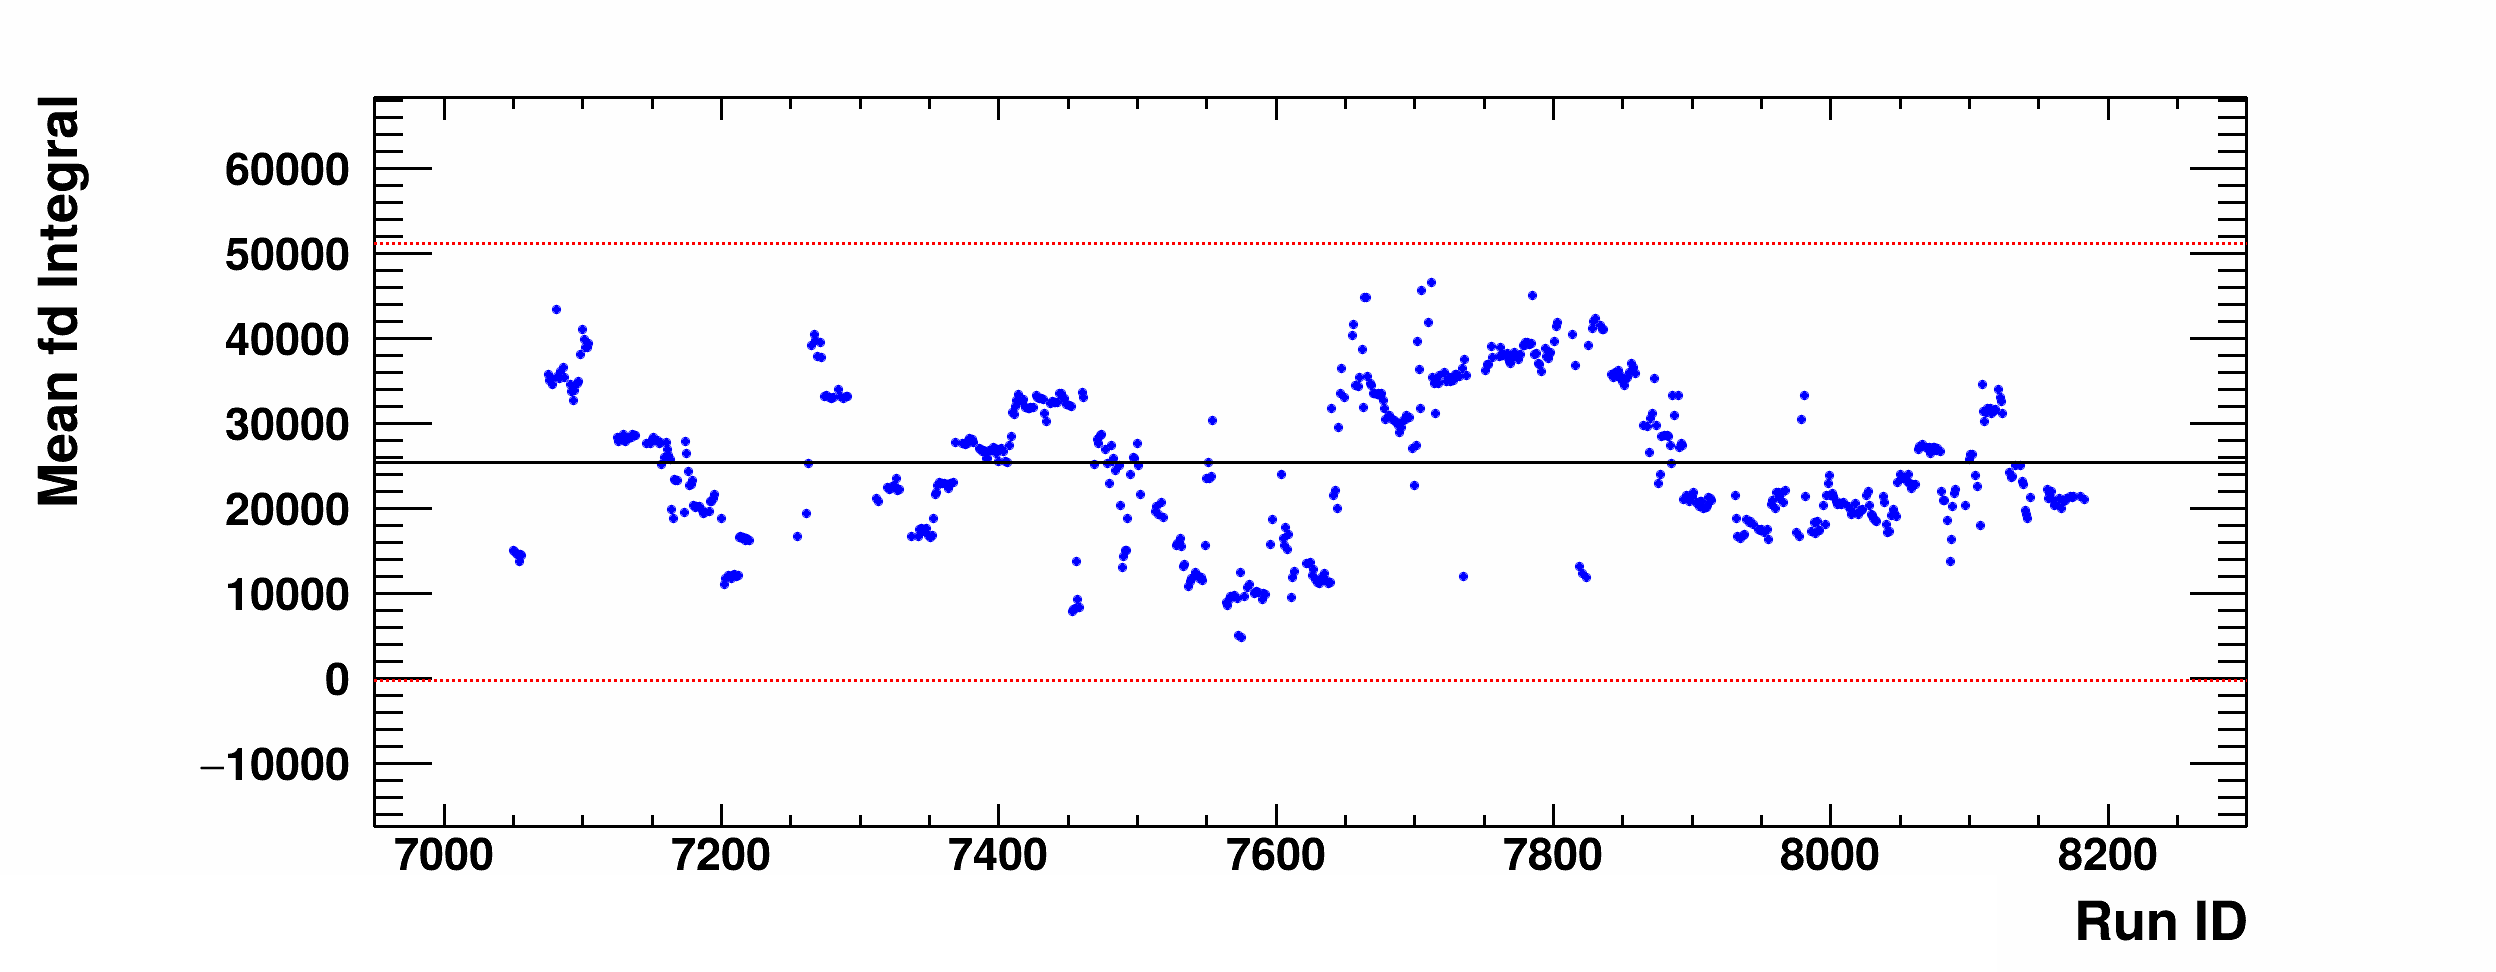
\includegraphics[width=0.60\linewidth]{../pict/QA_RunByRun_24.12/nVtxTr_h2_RunId_fdInt.png}
            \vspace{-3mm}
            \caption{Left panels: Distribution of the amplitude and integral of signal in the FD. The red marker corresponds to the distribution from the "outlier" RunId. Right panels: Mean amplitude and integral as a function RunID. Black dotted horizontal line and red horizontal lines represent $\mu$ and $\pm3\sigma$, respectively.}
            \label{fig:FD}
        \end{center}
        \vspace{-5mm}
    \end{figure}

    %============================= Fig ================================
    \begin{figure}[H]
        \begin{center}
            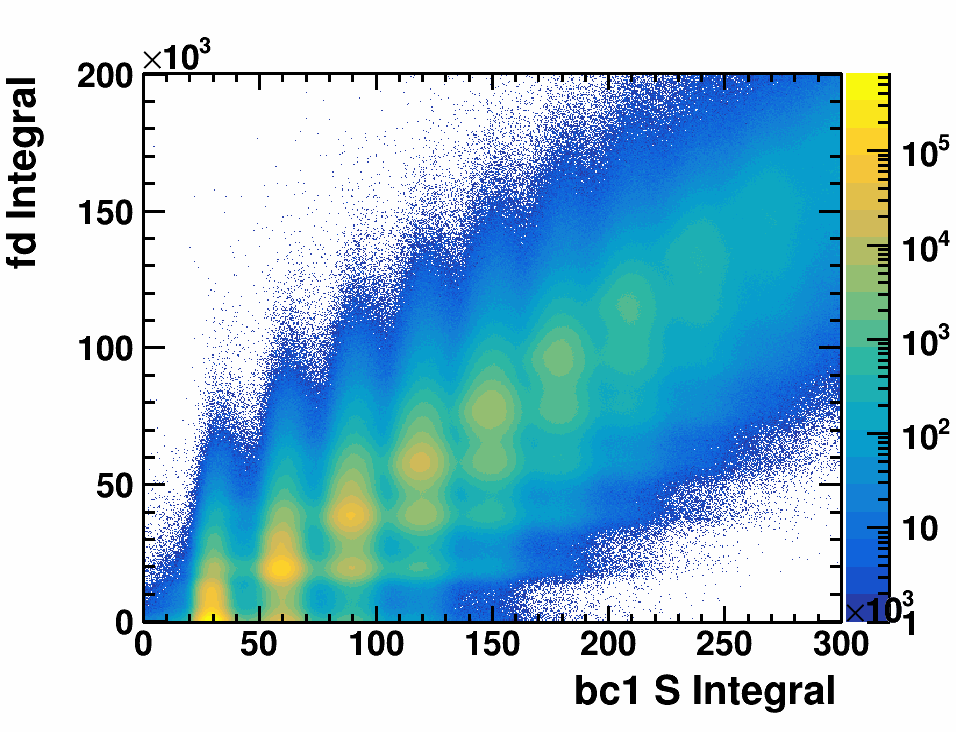
\includegraphics[width=0.49\linewidth]{QA_RunByRun_24.04_new/H2_NoRuns/cut5_h2_bc1sInt_fdInt.png}
            \vspace{-3mm}
            \caption{Correlation between the integral of the signal from the FD, and integral of the summed signal from the BC1.}
            \label{fig:bc1_vs_fd}
        \end{center}
        \vspace{-5mm}
    \end{figure}




\subsection{ Forward Hadron Calorimeter (FHCal)}

    
    Figures \ref{fig:FHCal},\ref{fig:FQH},\ref{fig:ScWall} shows the RunId dependence of the mean of the total energy 
    $E_{tot}$ of spectator fragments in the FHCal and mean of the charge ($Q^{2}$) 
    of spectator fragments in the forward quartz hodoscope (FQH) and scintillation wall (ScWall). Black dotted horizontal line and
    red horizontal lines represent $\mu$ and $\pm3\sigma$, respectively.

    %============================= Fig ================================
    \begin{figure}[H]
        \begin{center}
            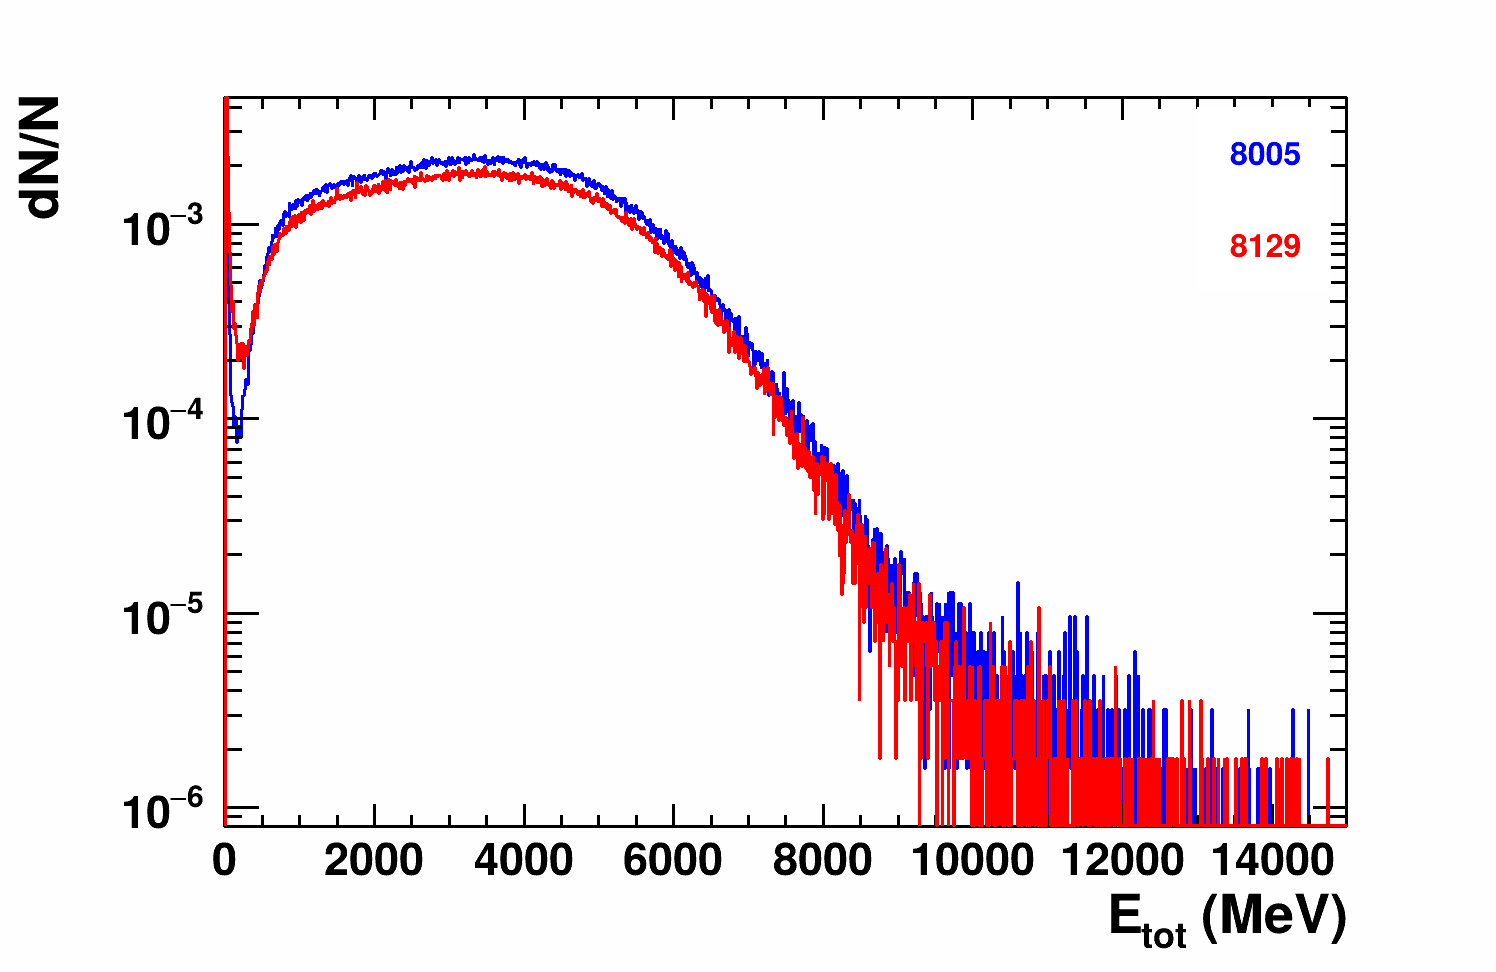
\includegraphics[width=0.35\linewidth]{../pict/QA_RunByRun_24.12/H1/nVtxTr_h2_RunId_fhcal_e.png}
            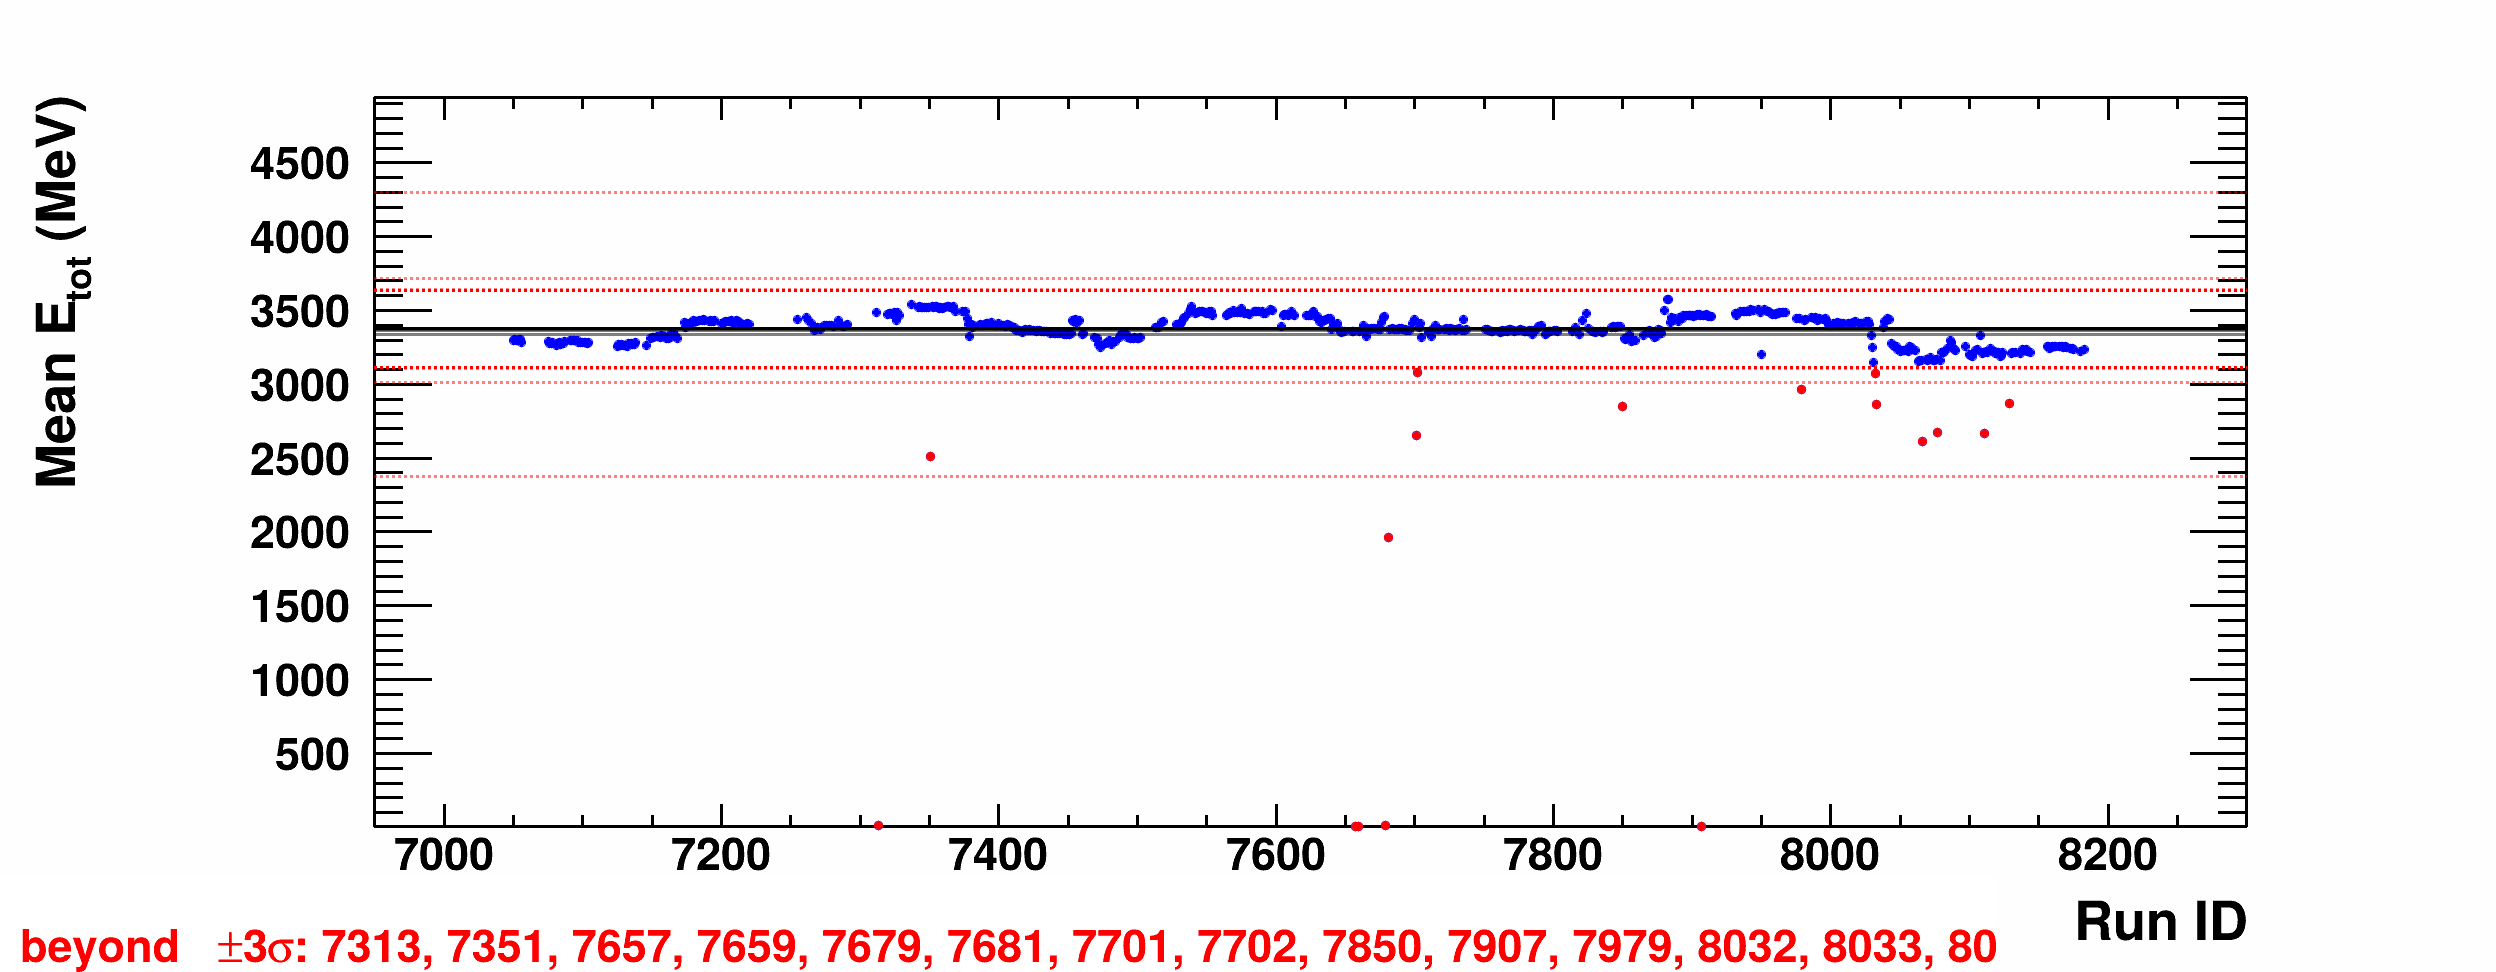
\includegraphics[width=0.60\linewidth]{../pict/QA_RunByRun_24.12/nVtxTr_h2_RunId_fhcal_e.png}
            \vspace{-3mm}
            \caption{Left panel: distribution of the total energy $E_{tot}$ of spectator fragments in the FHCal. The red marker corresponds to the distribution from the "outlier" RunId. Right panel: Mean $E_{tot}$ as a function RunID. Black dotted horizontal line and red horizontal lines represent $\mu$ and $\pm3\sigma$, respectively.}
            \label{fig:FHCal}
        \end{center}
        \vspace{-5mm}
    \end{figure}




\subsection{Forward Quartz Hodoscope (FQH)}

    %============================= Fig ================================
    \begin{figure}[H]
        \begin{center}
            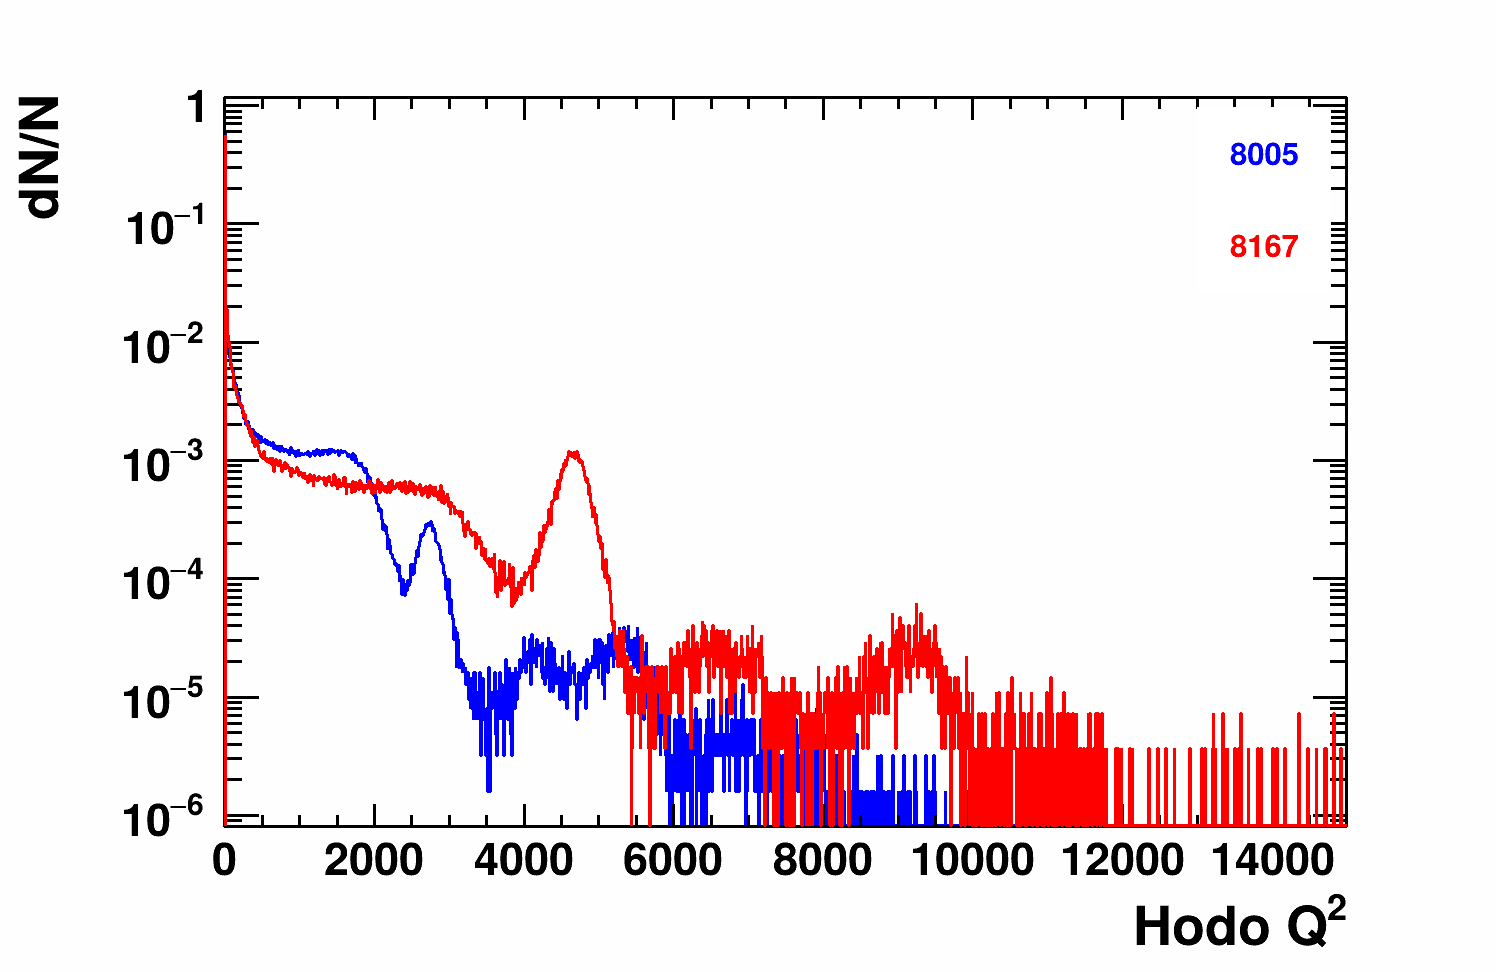
\includegraphics[width=0.35\linewidth]{../pict/QA_RunByRun_24.12/H1/nVtxTr_h2_RunId_hodo_q.png}
            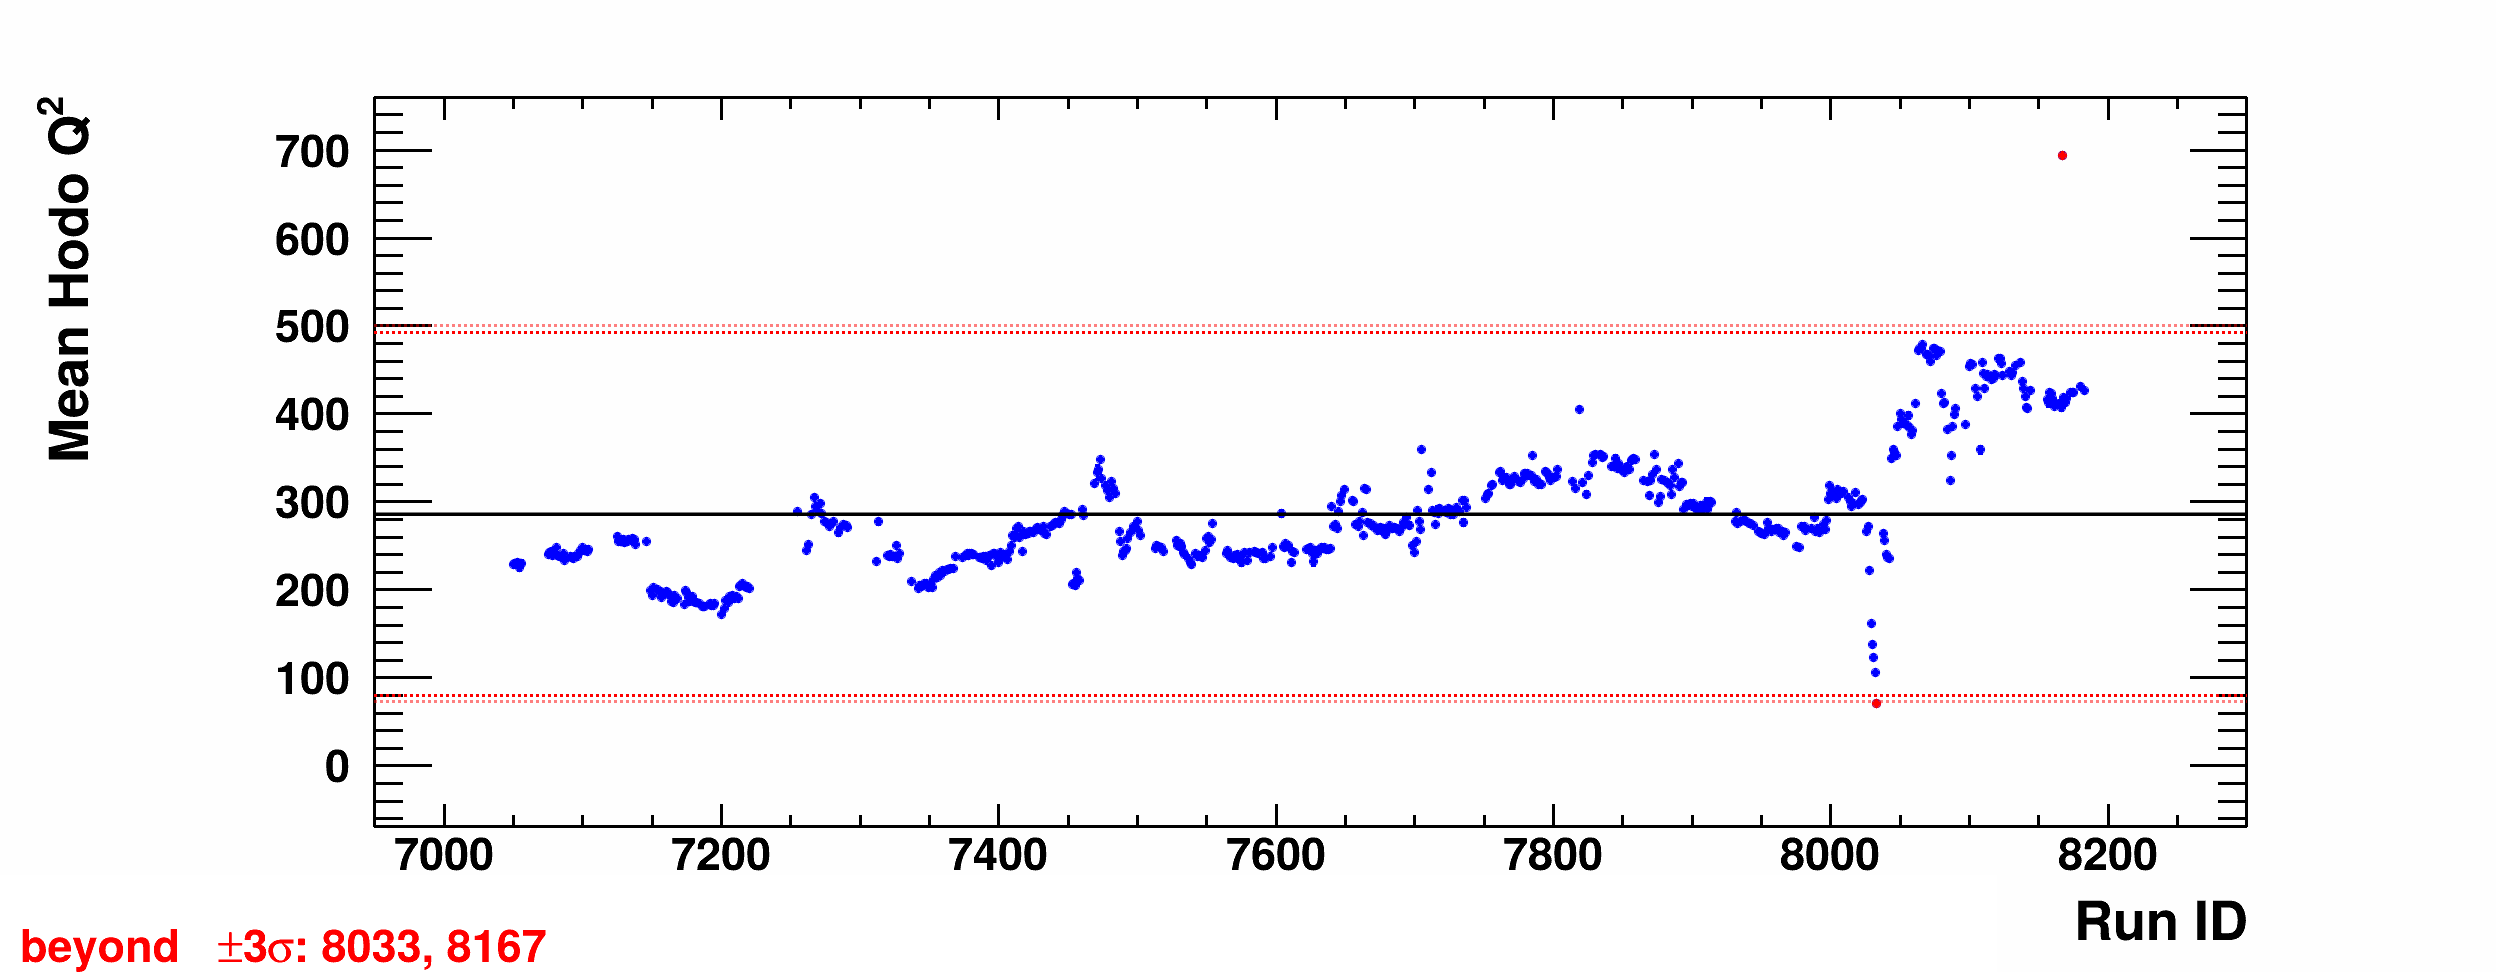
\includegraphics[width=0.60\linewidth]{../pict/QA_RunByRun_24.12/nVtxTr_h2_RunId_hodo_q.png}
            \vspace{-3mm}
            \caption{Left panel: distribution of the charge ($Q^2$) of spectator fragments in the forward quartz hodoscope (FQH). The red marker corresponds to the distribution from the "outlier" RunId. Right panel: Mean $Q^2$ as a function RunID. Black dotted horizontal line and red horizontal lines represent $\mu$ and $\pm3\sigma$, respectively.}
            \label{fig:FQH}
        \end{center}
        \vspace{-5mm}
    \end{figure}


\subsection{Scintillation Wall (ScWall)}

    %============================= Fig ================================
    \begin{figure}[H]
        \begin{center}
            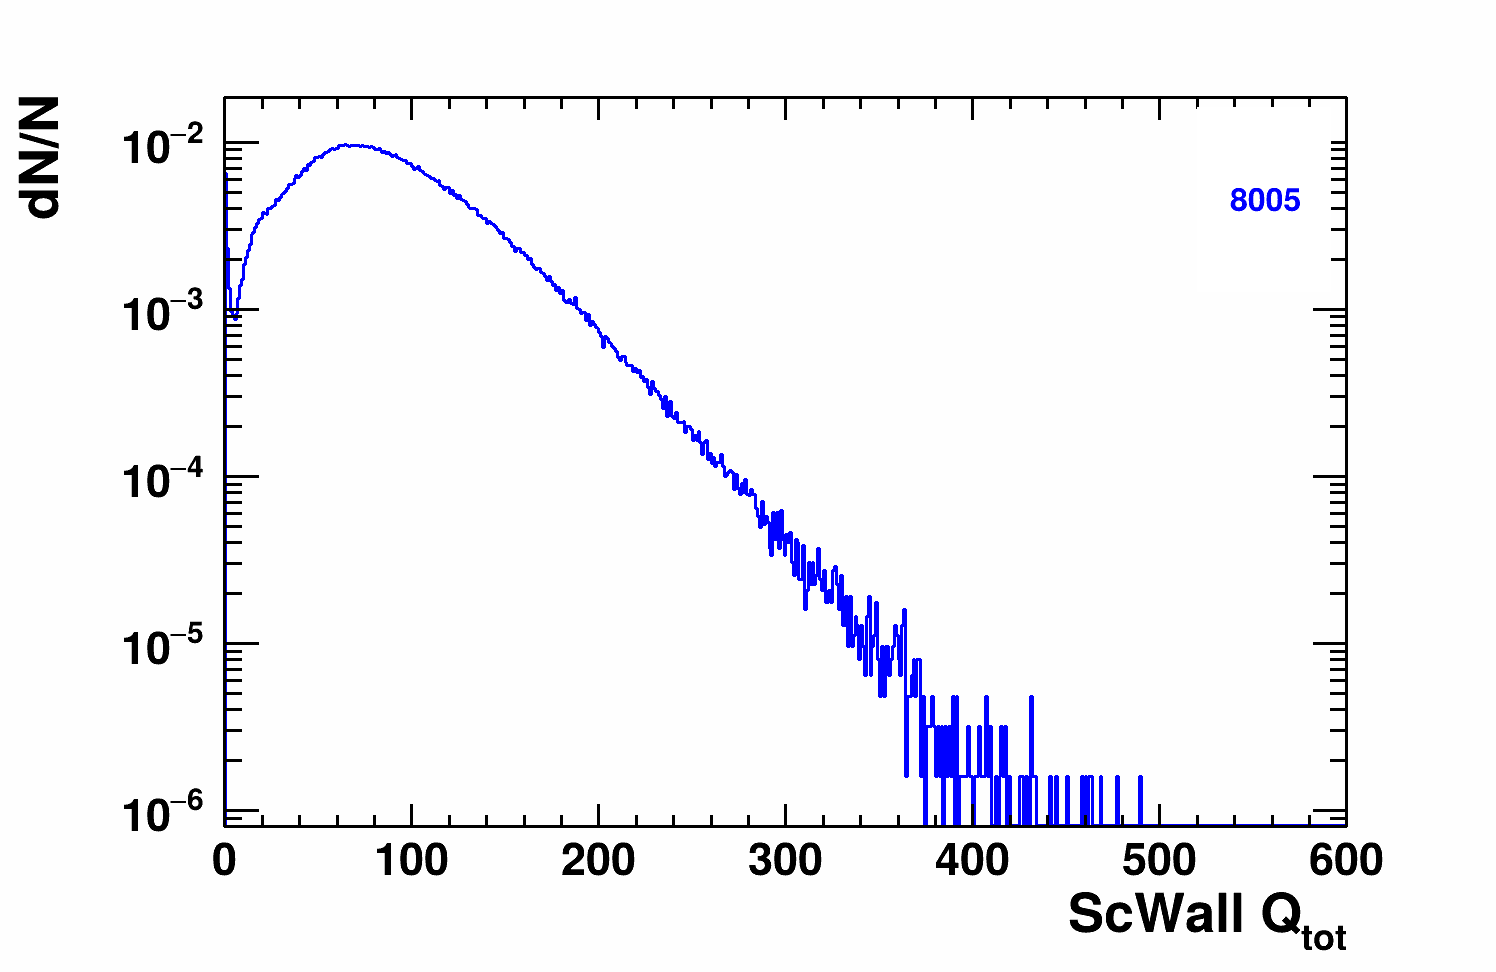
\includegraphics[width=0.35\linewidth]{../pict/QA_RunByRun_24.12/H1/nVtxTr_h2_RunId_scwall_q.png}
            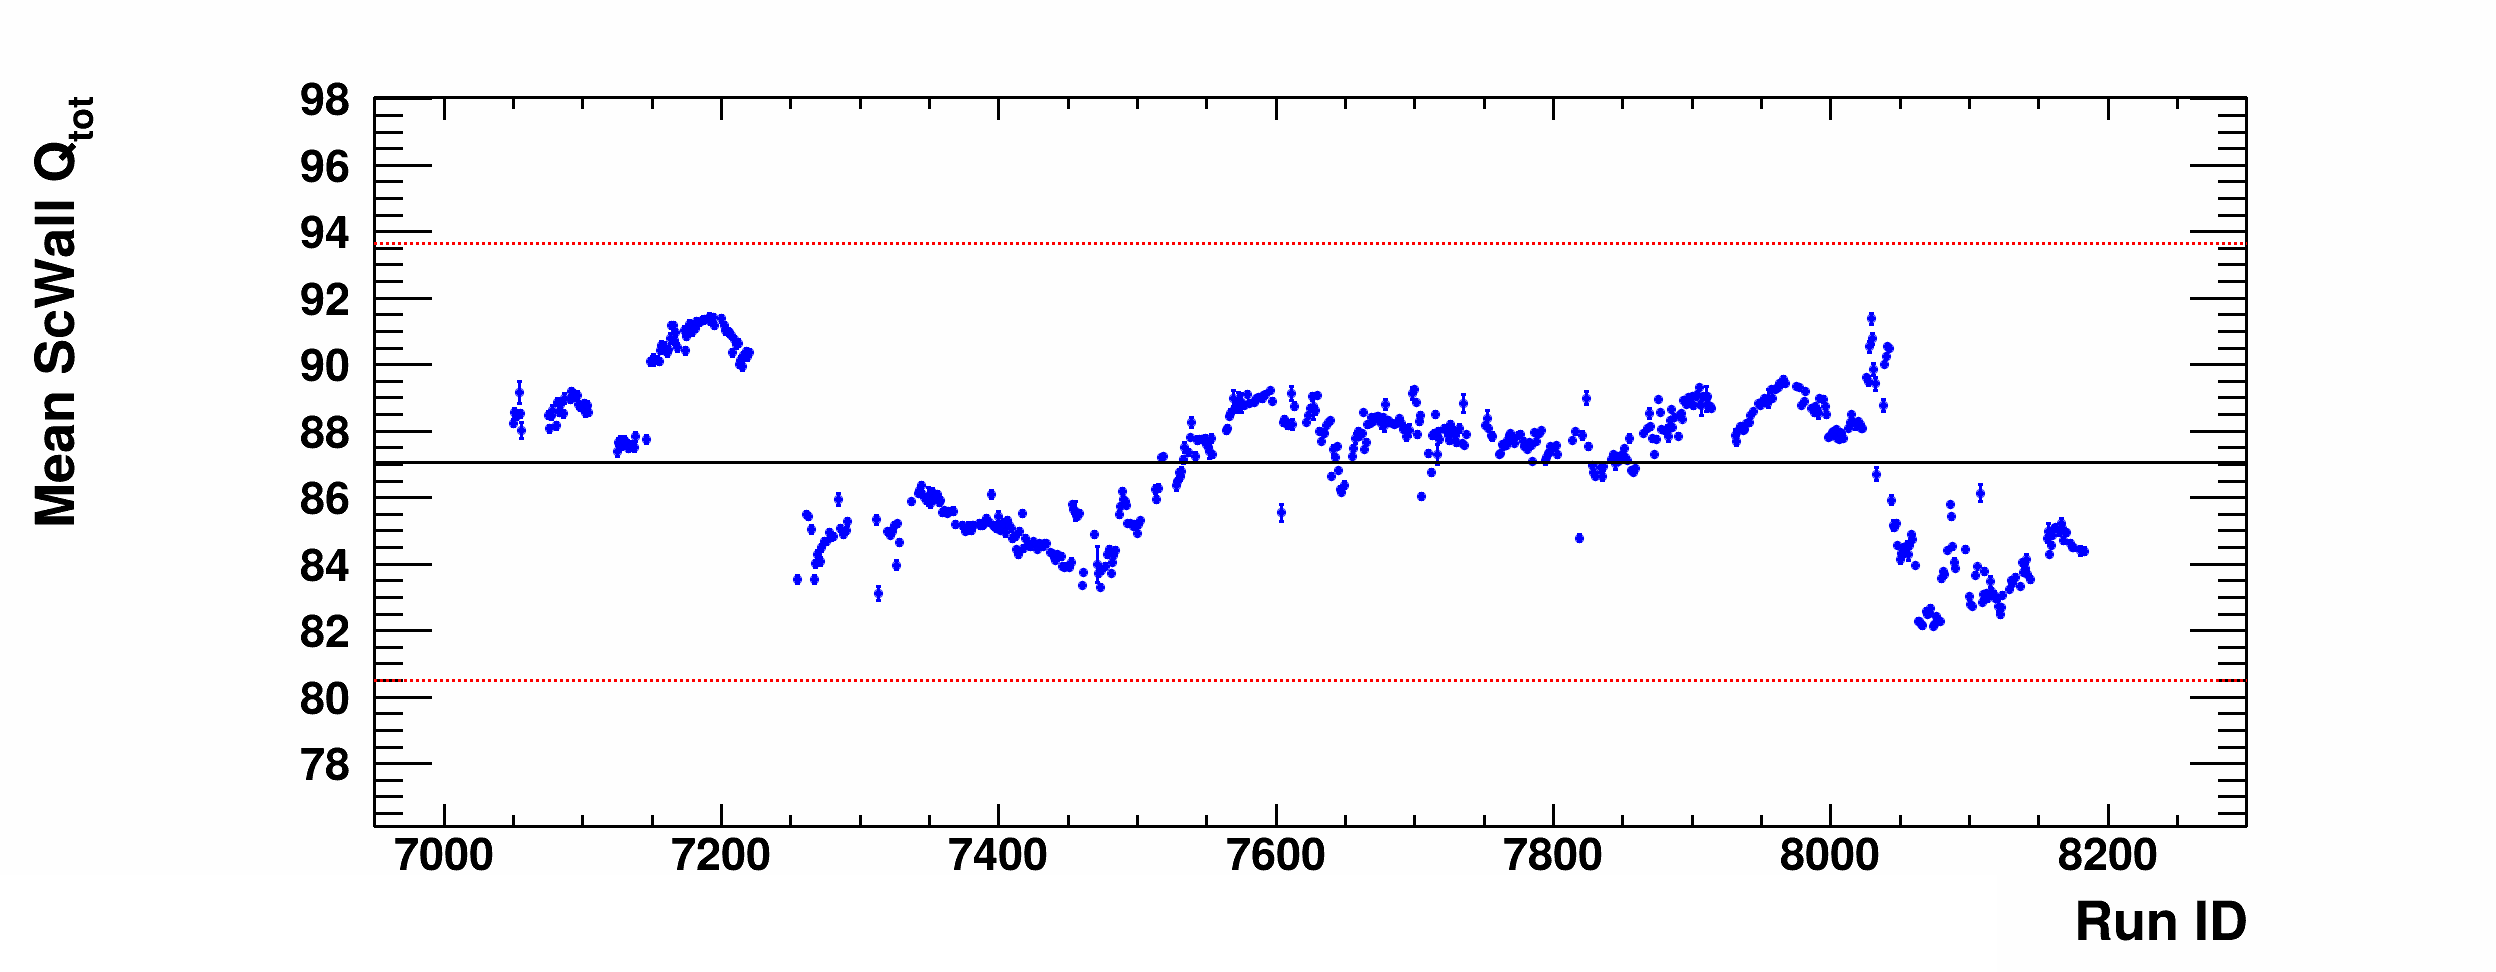
\includegraphics[width=0.60\linewidth]{../pict/QA_RunByRun_24.12/nVtxTr_h2_RunId_scwall_q.png}
            \vspace{-3mm}
            \caption{Left panel: distribution of the charge ($Q^2$) of spectator fragments in the ScWall. The red marker corresponds to the distribution from the "outlier" RunId. Right panel: Mean $Q^2$ as a function RunID. Black dotted horizontal line and red horizontal lines represent $\mu$ and $\pm3\sigma$, respectively.}
            \label{fig:ScWall}
        \end{center}
        \vspace{-5mm}
    \end{figure}


\subsection{Silicon Beam Tracker (SiBT)}

    Figure ~\ref{fig:SiBT} shows hits position in silicon beam tracker (SiBT) for three stations. 
    The lower panels of the figure are obtained from the upper ones by rotation by 0, 30 and 60 degrees.
    Figures ~\ref{fig:SiBT_x}-\ref{fig:SiBT_y} show the RunId dependence of the mean x and y hit positions for the three SiBT stations after rotation.
    Figure ~\ref{fig:SiBT_beam} show the RunId dependence the mean x and y of beam position in SiBT.

    %============================= Fig ================================
    \begin{figure}[H]
        \begin{center}
            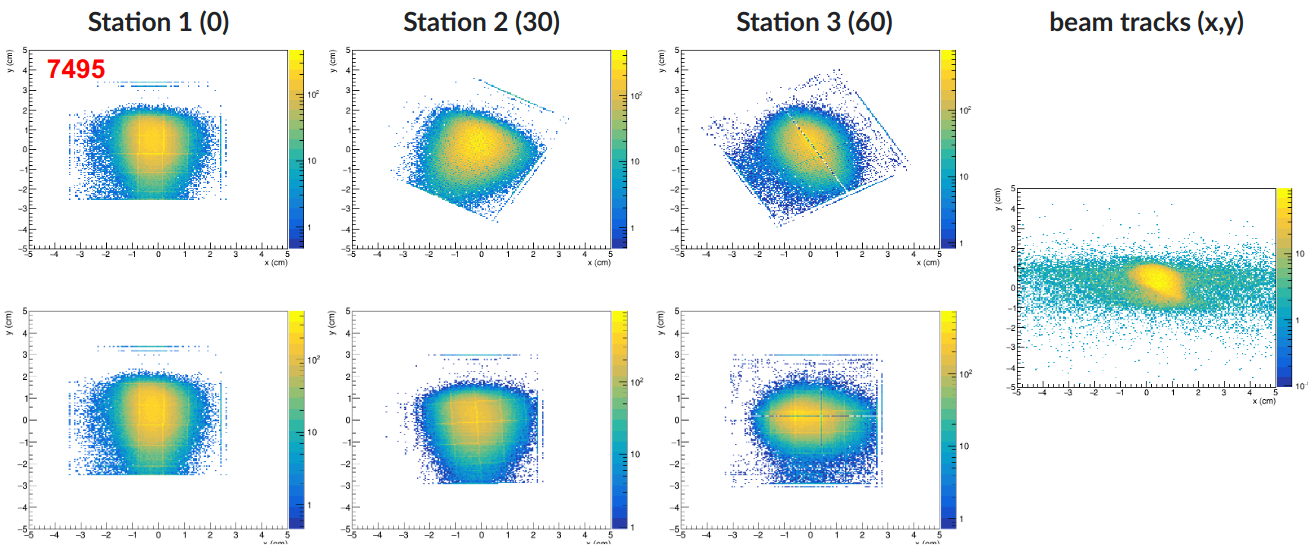
\includegraphics[width=0.9\linewidth]{../pict/QA_RunByRun_24.12/SiBT.png}
            \vspace{-3mm}
            \caption{Beam hits in three SiBT stations and reconstructed beam position}
            \label{fig:SiBT}
        \end{center}
        \vspace{-5mm}
    \end{figure}

    %============================= Fig ================================
    \begin{figure}[H]
        \begin{center}
            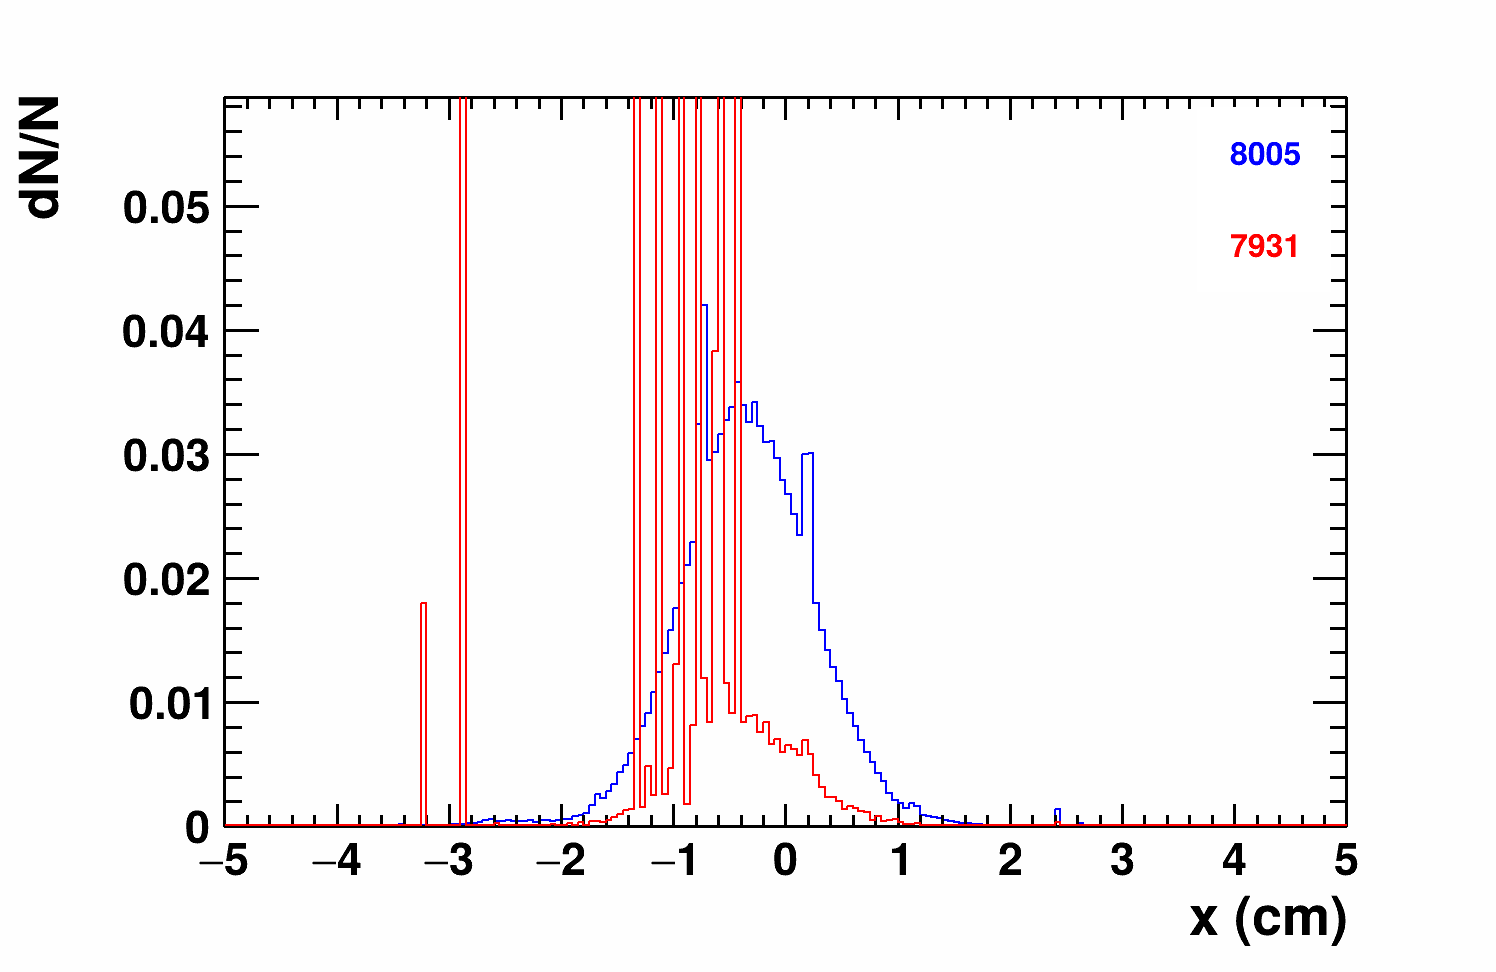
\includegraphics[width=0.35\linewidth]{../pict/QA_RunByRun_24.12/H1/nVtxTr_h2_RunId_beam_hit_x_st0.png}
            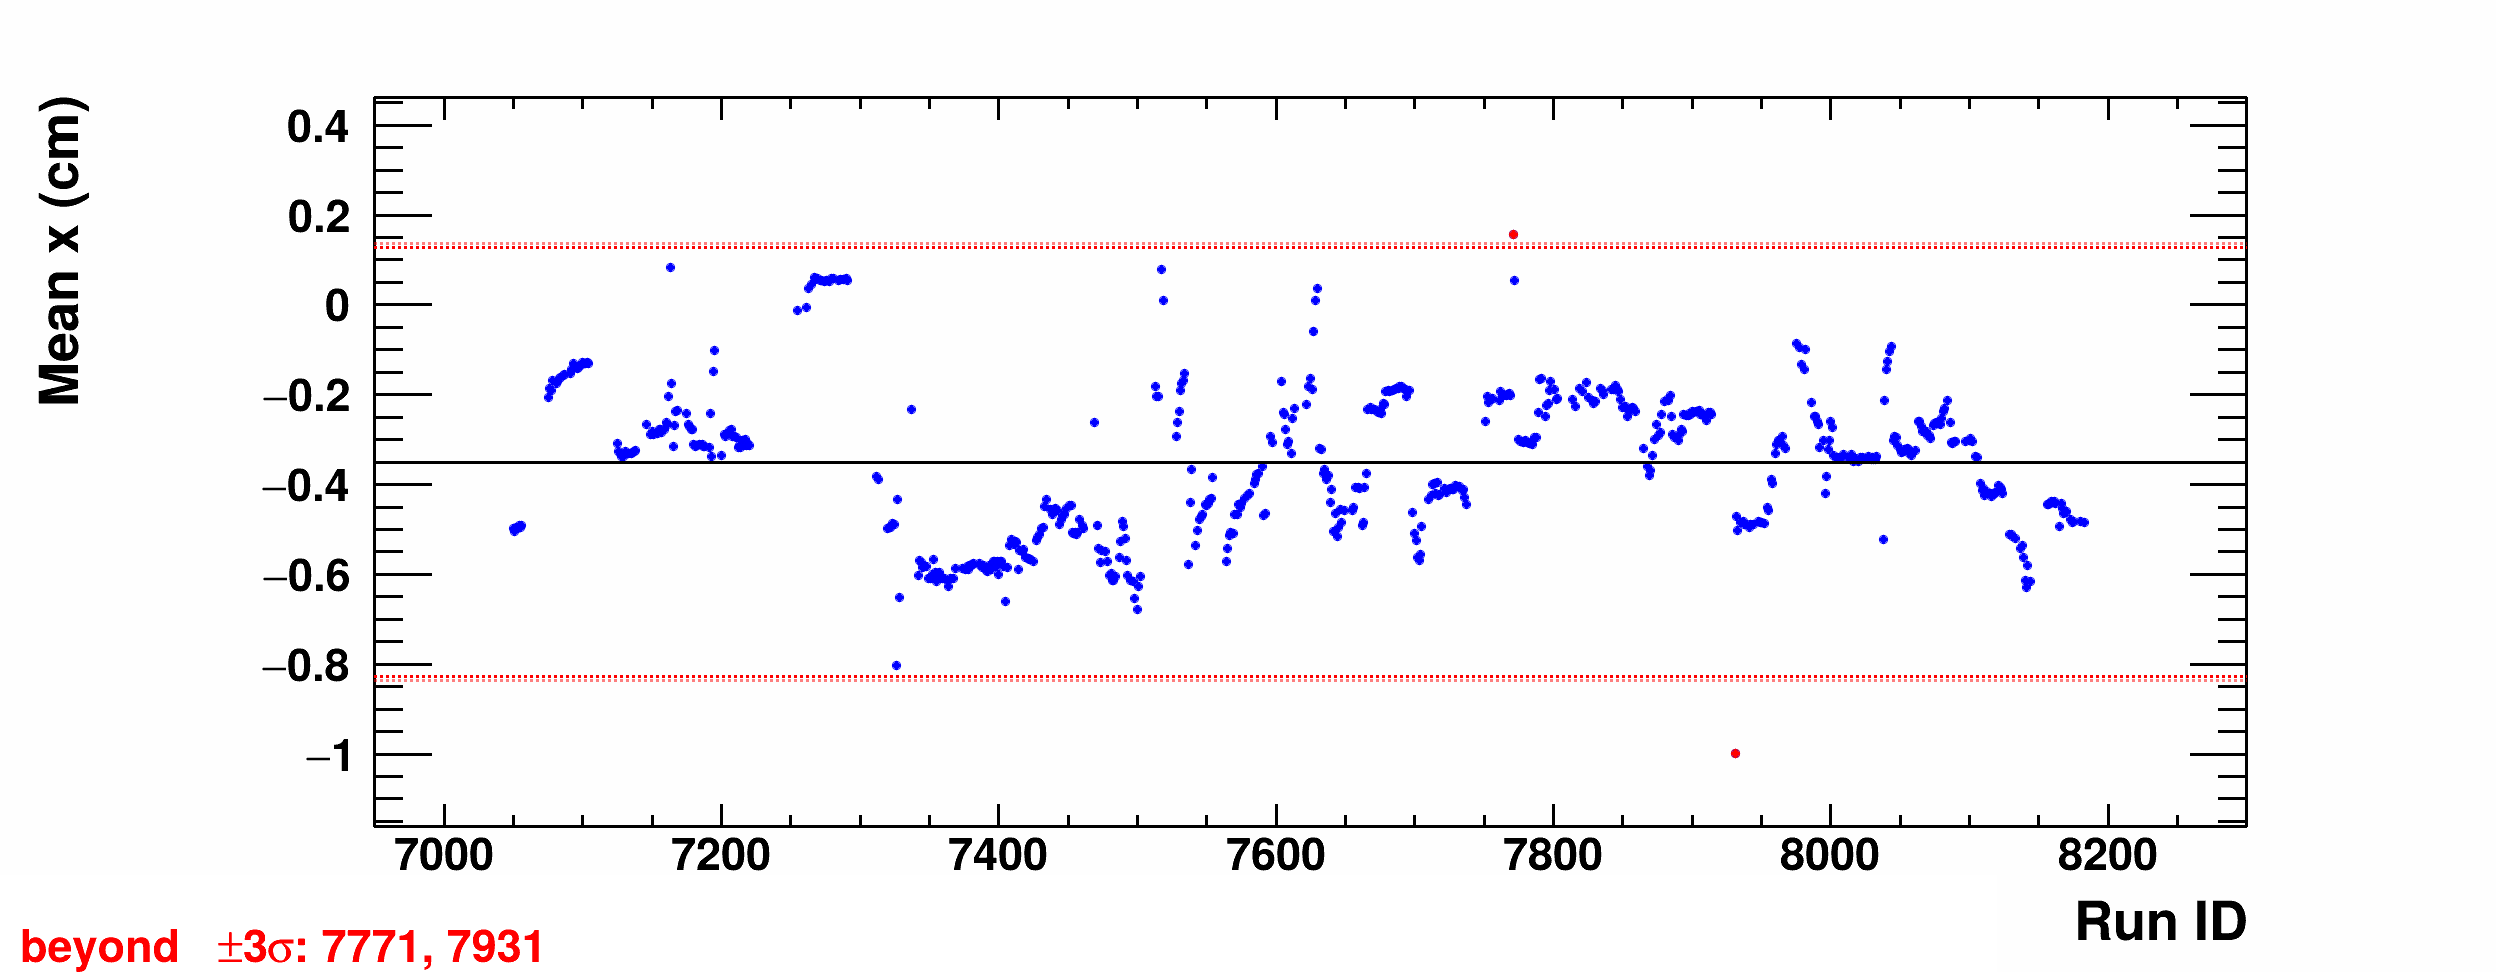
\includegraphics[width=0.60\linewidth]{../pict/QA_RunByRun_24.12/nVtxTr_h2_RunId_beam_hit_x_st0.png}

            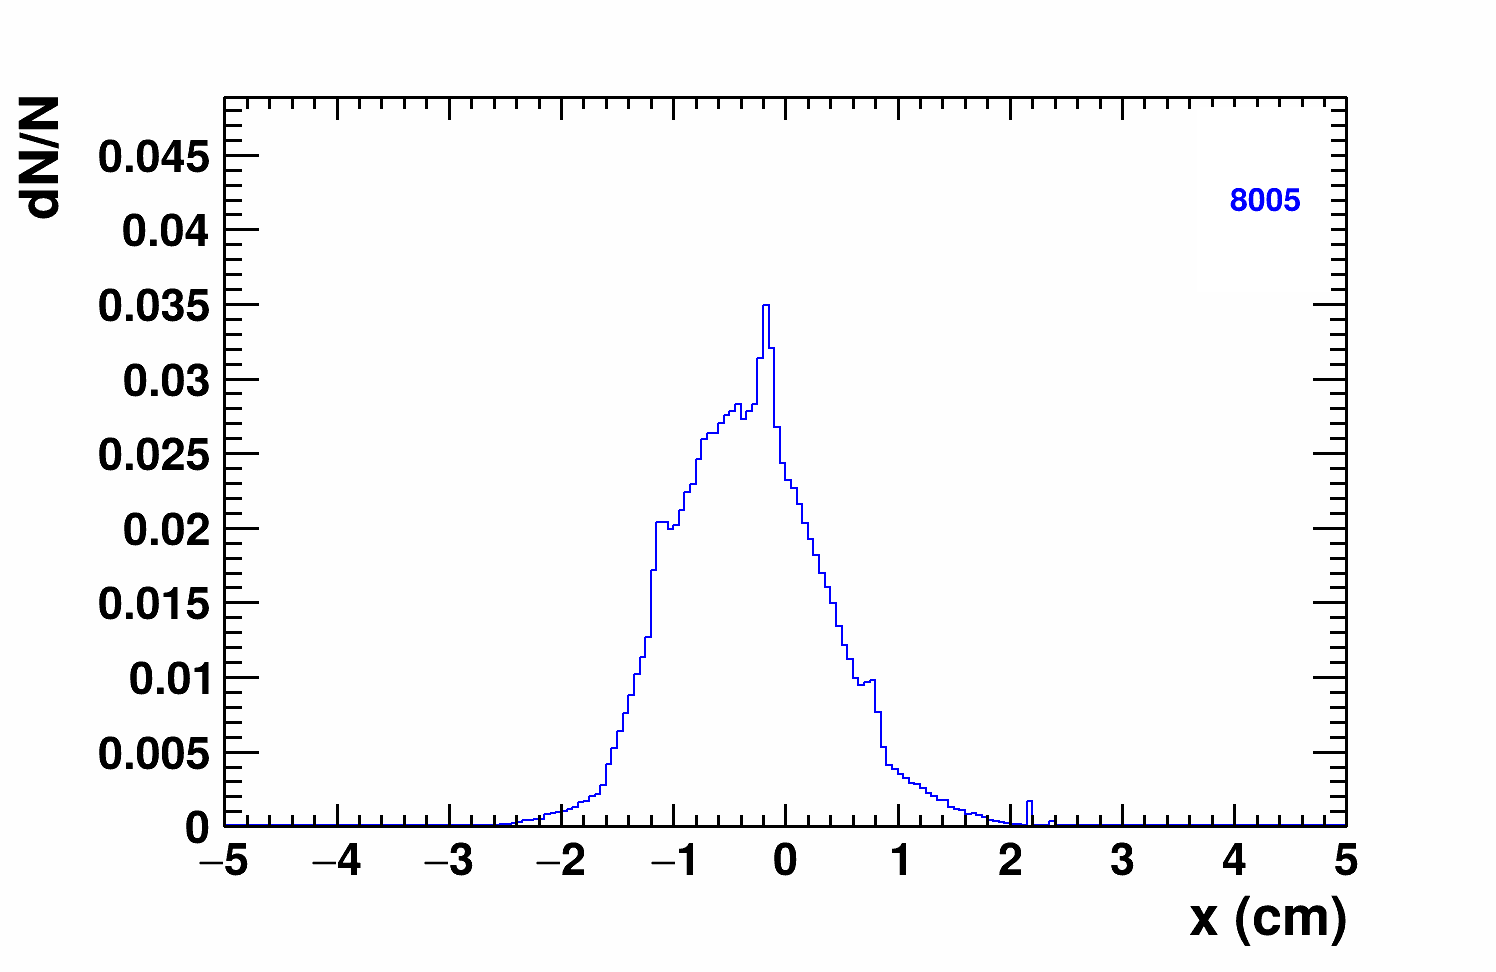
\includegraphics[width=0.35\linewidth]{../pict/QA_RunByRun_24.12/H1/nVtxTr_h2_RunId_beam_hit_x_st1.png}
            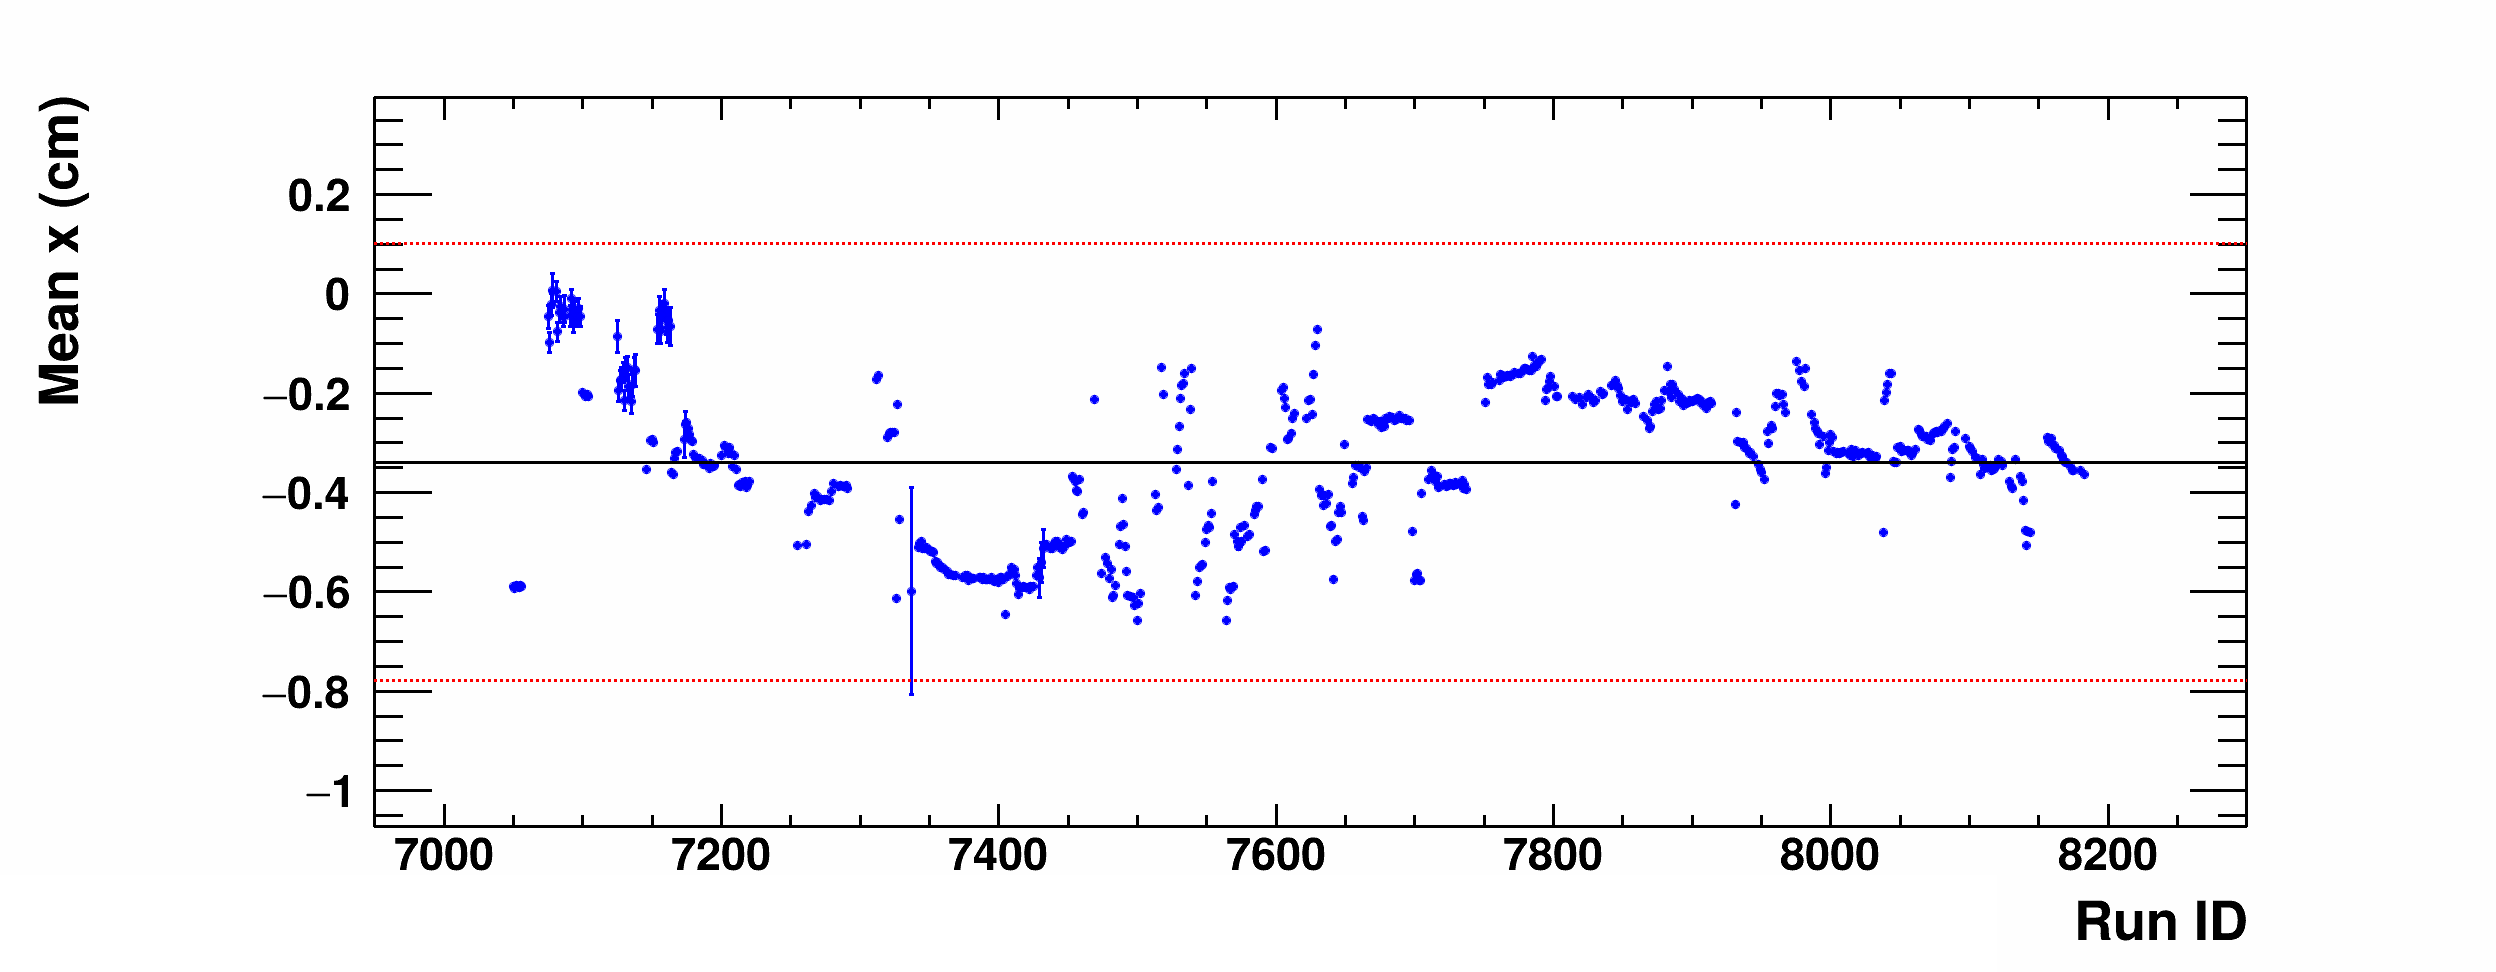
\includegraphics[width=0.60\linewidth]{../pict/QA_RunByRun_24.12/nVtxTr_h2_RunId_beam_hit_x_st1.png}

            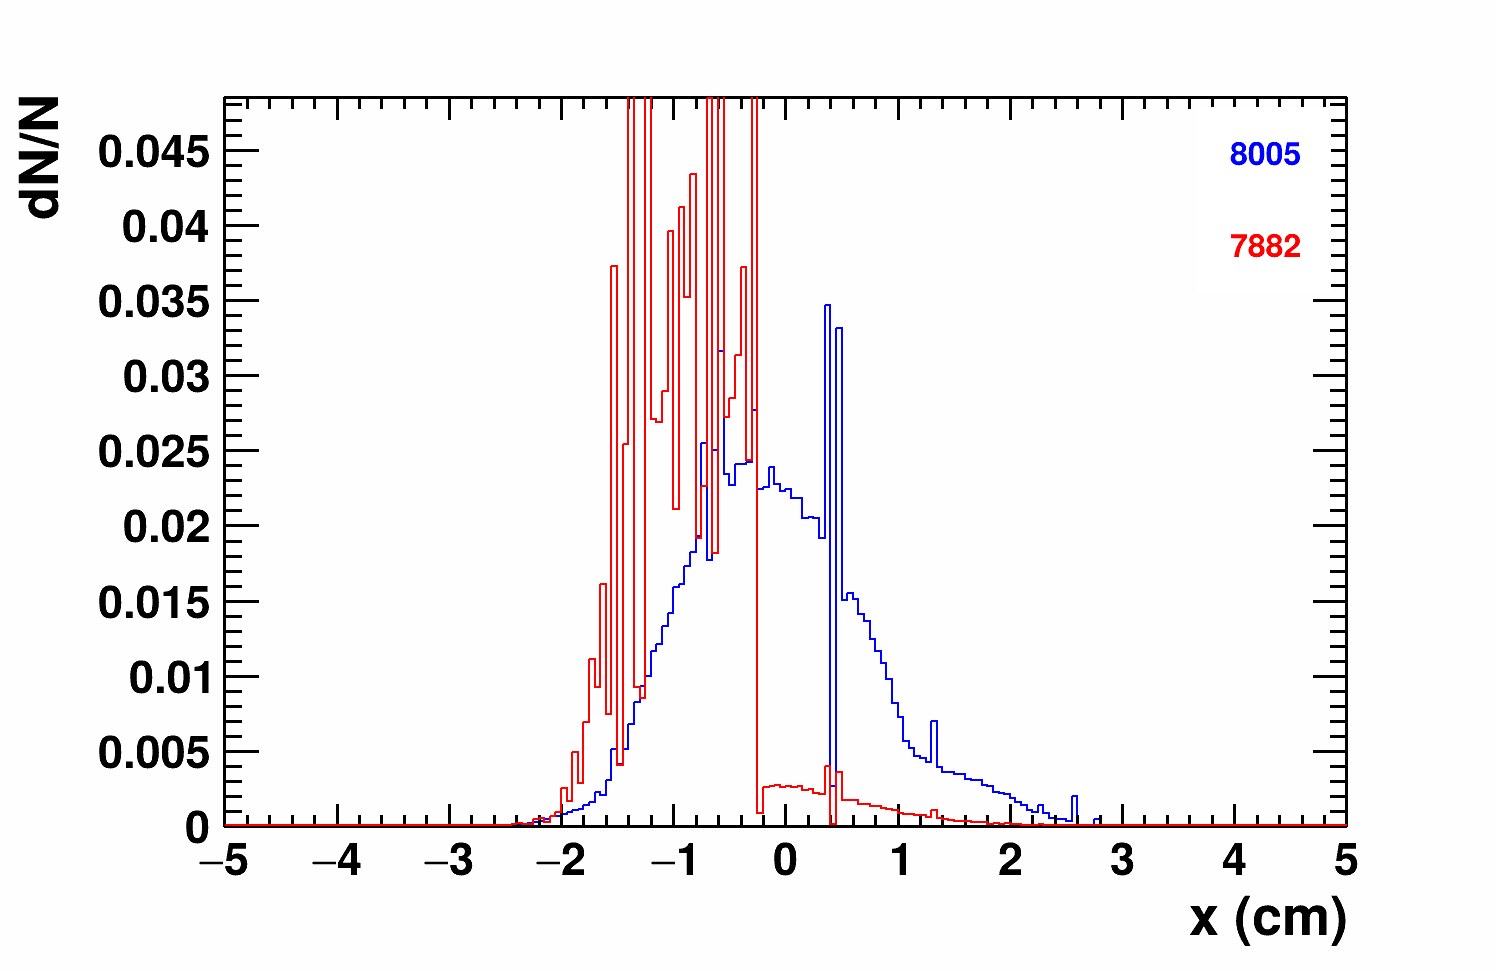
\includegraphics[width=0.35\linewidth]{../pict/QA_RunByRun_24.12/H1/nVtxTr_h2_RunId_beam_hit_x_st2.png}
            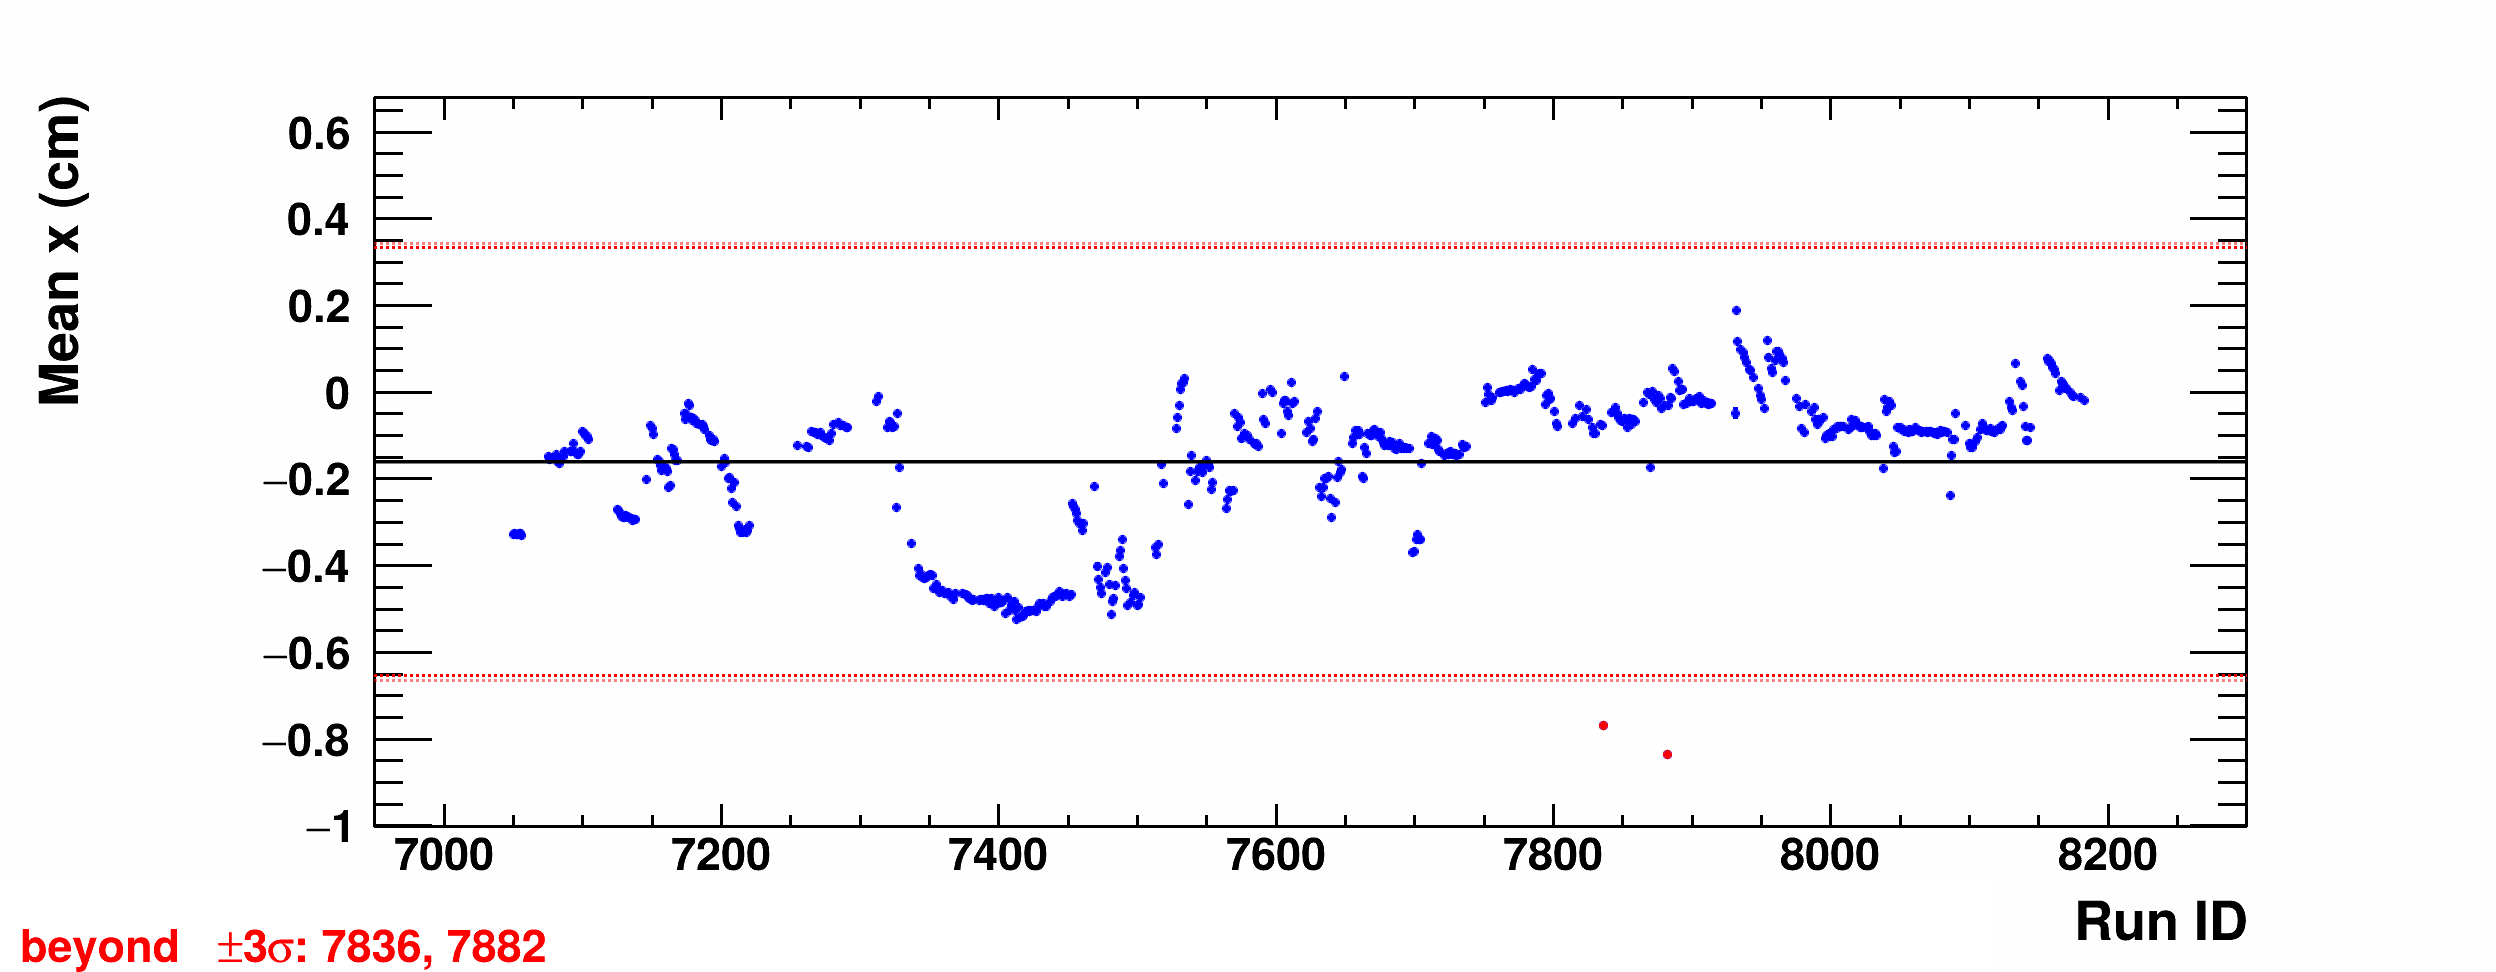
\includegraphics[width=0.60\linewidth]{../pict/QA_RunByRun_24.12/nVtxTr_h2_RunId_beam_hit_x_st2.png}

            \vspace{-3mm}
            \caption{Left panels: distribution of the x of hit beam position in 1,2 and 3 (from top to bottom respectively) SiBT stations. The red marker corresponds to the distribution from the "outlier" RunId. Right panels: Mean of the x of beam hit as a function RunID. Black dotted horizontal line and red horizontal lines represent $\mu$ and $\pm3\sigma$, respectively.}
            \label{fig:SiBT_x}
        \end{center}
        \vspace{-5mm}
    \end{figure}

    %============================= Fig ================================
    \begin{figure}[H]
        \begin{center}
            \includegraphics[width=0.35\linewidth]{../pict/QA_RunByRun_24.12/H1/nVtxTr_h2_RunId_beam_hit_y_st0.png}
            \includegraphics[width=0.60\linewidth]{../pict/QA_RunByRun_24.12/nVtxTr_h2_RunId_beam_hit_y_st0.png}

            \includegraphics[width=0.35\linewidth]{../pict/QA_RunByRun_24.12/H1/nVtxTr_h2_RunId_beam_hit_y_st1.png}
            \includegraphics[width=0.60\linewidth]{../pict/QA_RunByRun_24.12/nVtxTr_h2_RunId_beam_hit_y_st1.png}

            \includegraphics[width=0.35\linewidth]{../pict/QA_RunByRun_24.12/H1/nVtxTr_h2_RunId_beam_hit_y_st2.png}
            \includegraphics[width=0.60\linewidth]{../pict/QA_RunByRun_24.12/nVtxTr_h2_RunId_beam_hit_y_st2.png}

            \vspace{-3mm}
            \caption{Left panels: distribution of the y of hit beam position in 1,2 and 3 (from top to bottom respectively) SiBT stations. The red marker corresponds to the distribution from the "outlier" RunId. Right panels: Mean of the y of beam hit as a function RunID. Black dotted horizontal line and red horizontal lines represent $\mu$ and $\pm3\sigma$, respectively.}
            \label{fig:SiBT_y}
        \end{center}
        \vspace{-5mm}
    \end{figure}

    %============================= Fig ================================
    \begin{figure}[H]
        \begin{center}
            \includegraphics[width=0.35\linewidth]{../pict/QA_RunByRun_24.12/H1/nVtxTr_h2_RunId_beam_x.png}
            \includegraphics[width=0.60\linewidth]{../pict/QA_RunByRun_24.12/nVtxTr_h2_RunId_beam_x.png}

            \includegraphics[width=0.35\linewidth]{../pict/QA_RunByRun_24.12/H1/nVtxTr_h2_RunId_beam_y.png}
            \includegraphics[width=0.60\linewidth]{../pict/QA_RunByRun_24.12/nVtxTr_h2_RunId_beam_y.png}

            \vspace{-3mm}
            \caption{Left panels: distribution of the x and y of beam position in SiBT. The red marker corresponds to the distribution from the "outlier" RunId. Right panels: Mean of the x,y of beam position in SiBT as a function RunID. Black dotted horizontal line and red horizontal lines represent $\mu$ and $\pm3\sigma$, respectively.}
            \label{fig:SiBT_beam}
        \end{center}
        \vspace{-5mm}
    \end{figure}


\subsection{Global tracks}

    %============================= Fig ================================
    \begin{figure}[H]
        \begin{center}
            \includegraphics[width=0.35\linewidth]{../pict/QA_RunByRun_24.12/H1/nVtxTr_h2_RunId_tr_px.png}
            \includegraphics[width=0.60\linewidth]{../pict/QA_RunByRun_24.12/nVtxTr_h2_RunId_tr_px.png}

            \includegraphics[width=0.35\linewidth]{../pict/QA_RunByRun_24.12/H1/nVtxTr_h2_RunId_tr_py.png}
            \includegraphics[width=0.60\linewidth]{../pict/QA_RunByRun_24.12/nVtxTr_h2_RunId_tr_py.png}

            \includegraphics[width=0.35\linewidth]{../pict/QA_RunByRun_24.12/H1/nVtxTr_h2_RunId_tr_pz.png}
            \includegraphics[width=0.60\linewidth]{../pict/QA_RunByRun_24.12/nVtxTr_h2_RunId_tr_pz.png}
            \vspace{-3mm}
            \caption{Left panels: Distribution of the x,y and z component of momentum of charged particles. The red marker corresponds to the distribution from the "outlier" RunId. Right panels: Mean x,y and z component of momentum as a function RunID. Black dotted horizontal line and red horizontal lines represent $\mu$ and $\pm3\sigma$, respectively.}
        \end{center}
        \label{Momentum}
        \vspace{-5mm}
    \end{figure}

    %============================= Fig ================================
    \begin{figure}[H]
        \begin{center}
            \includegraphics[width=0.35\linewidth]{../pict/QA_RunByRun_24.12/H1/nVtxTr_h2_RunId_tr_pT.png}
            \includegraphics[width=0.60\linewidth]{../pict/QA_RunByRun_24.12/nVtxTr_h2_RunId_tr_pT.png}

            \includegraphics[width=0.35\linewidth]{../pict/QA_RunByRun_24.12/H1/nVtxTr_h2_RunId_tr_phi.png}
            \includegraphics[width=0.60\linewidth]{../pict/QA_RunByRun_24.12/nVtxTr_h2_RunId_tr_phi.png}

            \includegraphics[width=0.35\linewidth]{../pict/QA_RunByRun_24.12/H1/nVtxTr_h2_RunId_tr_eta.png}
            \includegraphics[width=0.60\linewidth]{../pict/QA_RunByRun_24.12/nVtxTr_h2_RunId_tr_eta.png}
            \vspace{-3mm}
            \caption{Upper panels: Distribution of the transverse momentum (upper), azimuthal angle (center) and rapidity (bottom) of charged particles. The red marker corresponds to the distribution from the "outlier" RunId. Bottom panels: Mean $p_T$, $\phi$ and $\eta$ as a function RunID. Black dotted horizontal line and red horizontal lines represent $\mu$ and $\pm3\sigma$, respectively.}
        \end{center}
        \label{track_par}
        \vspace{-5mm}
    \end{figure}

    %============================= Fig ================================
    \begin{figure}[H]
        \begin{center}
            \includegraphics[width=0.35\linewidth]{../pict/QA_RunByRun_24.12/H1/nVtxTr_h2_RunId_tr_nhits.png}
            \includegraphics[width=0.60\linewidth]{../pict/QA_RunByRun_24.12/nVtxTr_h2_RunId_tr_nhits.png}

            \includegraphics[width=0.35\linewidth]{../pict/QA_RunByRun_24.12/H1/nVtxTr_h2_RunId_tr_dca_r.png}
            \includegraphics[width=0.60\linewidth]{../pict/QA_RunByRun_24.12/nVtxTr_h2_RunId_tr_dca_r.png}
            \vspace{-3mm}
            \caption{Left panels: Distribution of the number of fit points in to accurate track momentum reconstruction (upper) and the distance of closest approach $DCA_R$ (bottom). The red marker corresponds to the distribution from the "outlier" RunId. Right panels: Mean nHits and $DCA_R$ as a function RunID. Black dotted horizontal line and red horizontal lines represent $\mu$ and $\pm3\sigma$, respectively.}
        \end{center}
        \label{nHits_dca}
        \vspace{-5mm}
    \end{figure}

    %============================= Fig ================================
    \begin{figure}[H]
        \begin{center}
            \includegraphics[width=0.32\linewidth]{../pict/QA_RunByRun_24.12/H2_NoRuns/cut5_h2_tr_phi_tr_eta.png}
            \includegraphics[width=0.32\linewidth]{../pict/QA_RunByRun_24.12/H2_NoRuns/cut5_h2_tr_pT_tr_eta.png}
            \includegraphics[width=0.32\linewidth]{../pict/QA_RunByRun_24.12/H2_NoRuns/cut5_h2_tr_pT_tr_phi.png}
            \vspace{-3mm}
            \caption{Correlation between the $\eta$ and the $\phi$ (left), $\eta$ and $p_T$ (center), $\phi$ and $p_T$ (right).}
        \end{center}
        \label{nHits_dca}
        \vspace{-5mm}
    \end{figure}




\subsection{Mass squared distribution}\label{m2_qa_sec}

    %============================= Fig ================================
    \begin{figure}[H]
        \begin{center}
            \includegraphics[width=0.49\linewidth]{../pict/QA_RunByRun_24.12/H2_NoRuns/cut5_h2_tr_pq_tr_m2_tof400.png}
            \includegraphics[width=0.49\linewidth]{../pict/QA_RunByRun_24.12/H2_NoRuns/cut5_h2_tr_pq_tr_m2_tof700.png}
            \vspace{-3mm}
            \caption{Correlation between the mass squared ($m^2$) and rigidity ($p/q$) in the TOF-400 (left panel) and TOF-700 (right panel) detectors.}
        \end{center}
        \label{m2_TOF}
        \vspace{-5mm}
    \end{figure}

    %============================= Fig ================================
    \begin{figure}[H]
        \begin{center}
            \includegraphics[width=0.9\linewidth]{../pict/QA_RunByRun_24.12/proton_m2.png}
            \vspace{-3mm}
            \caption{Distribution of the mass squared ($m^2$) and Gaussian fit of the proton peak in the TOF-400 (upper panels) and TOF-700 (bottom panels) detectors. Center and right panels: mean of the mass squared of proton and $\sigma_{p}$ as a function RunID. Black dotted horizontal line and red horizontal lines represent $\mu$ and $\pm3\sigma$, respectively. }
        \end{center}
        \label{mass2_proton}
        \vspace{-5mm}
    \end{figure}

    %============================= Fig ================================
    \begin{figure}[H]
        \begin{center}
            \includegraphics[width=0.9\linewidth]{../pict/QA_RunByRun_24.12/pion_plus_m2.png}
            \vspace{-3mm}
            \caption{Distribution of the mass squared ($m^2$) and Gaussian fit of the $\pi^{+}$ peak in the TOF-400 (upper panels) and TOF-700 (bottom panels) detectors. Center and right panels: the mass squared of $\pi^{+}$ and $\sigma$ as a function RunID. Black dotted horizontal line and red horizontal lines represent $\mu$ and $\pm3\sigma$, respectively.}
        \end{center}
        \label{mass2_proton}
        \vspace{-5mm}
    \end{figure}

        %============================= Fig ================================
    \begin{figure}[H]
        \begin{center}
            \includegraphics[width=0.9\linewidth]{../pict/QA_RunByRun_24.12/pion_minus_m2.png}
            \vspace{-3mm}
            \caption{Distribution of the mass squared ($m^2$) and Gaussian fit of the $\pi^{-}$ peak in the TOF-400 (upper panels) and TOF-700 (bottom panels) detectors. Center and right panels: the mass squared of $\pi^{-}$ and $\sigma$ as a function RunID. Black dotted horizontal line and red horizontal lines represent $\mu$ and $\pm3\sigma$, respectively.}
        \end{center}
        \label{mass2_proton}
        \vspace{-5mm}
    \end{figure}

    % Phisical Runs: 6667, 6668, 6669, 6670, 6671, 6672, 6673, 6674, 6675, 6676, 6677, 6678, 6679, 6680, 6681, 6683, 6684, 6685, 6686, 6687, 6689, 6690, 6691, 6692, 6694, 6695, 6696, 6698, 6699, 6732, 6733, 6734, 6737, 6738, 6739, 6740, 6745, 6752, 6753, 6760, 6761, 6765, 6766, 6767, 6768, 6769, 6771, 6772, 6773, 6774, 6779, 6780, 6782, 6783, 6785, 6786, 6788, 6794, 6795, 6797, 6799, 6800, 6803, 6815, 6816, 6817, 6818, 6819, 6820, 6821, 6822, 6879, 6882, 6883, 6884, 6886, 6887, 6889, 6891, 6900, 6901, 6902, 6903, 6904, 6905, 6906, 6907, 6908, 6909, 6910, 6911, 6915, 6916, 6918, 6919, 6920, 6921, 6923, 6924, 6926, 6927, 6928, 6929, 6930, 6931, 6932, 6933, 6934, 6935, 6936, 6937, 6939, 6940, 6968, 6970, 6972, 6973, 6975, 6976, 6977, 6978, 6979, 6980, 6981, 6982, 6983, 6984, 6990, 6991, 6992, 6993, 6994, 6995, 6997, 6998, 6999, 7000, 7002, 7003, 7004, 7005, 7006, 7008, 7009, 7010, 7011, 7012, 7030, 7031, 7032, 7033, 7034, 7035, 7037, 7038, 7040, 7041, 7042, 7043, 7044, 7046, 7047, 7048, 7049, 7050, 7051, 7052, 7053, 7054, 7055, 7056, 7075, 7076, 7077, 7078, 7081, 7082, 7083, 7084, 7086, 7087, 7091, 7092, 7093, 7094, 7096, 7097, 7098, 7100, 7101, 7102, 7103, 7104, 7125, 7126, 7127, 7128, 7129, 7130, 7131, 7132, 7133, 7135, 7136, 7137, 7138, 7146, 7149, 7150, 7151, 7154, 7155, 7156, 7157, 7159, 7160, 7161, 7162, 7163, 7164, 7165, 7166, 7167, 7168, 7173, 7174, 7175, 7176, 7177, 7178, 7179, 7180, 7181, 7182, 7184, 7186, 7187, 7188, 7191, 7192, 7193, 7194, 7195, 7200, 7202, 7203, 7205, 7206, 7207, 7208, 7209, 7211, 7212, 7213, 7214, 7215, 7216, 7217, 7218, 7219, 7220, 7223, 7225, 7255, 7258, 7261, 7263, 7265, 7267, 7268, 7269, 7271, 7272, 7274, 7276, 7278, 7279, 7281, 7284, 7286, 7288, 7290, 7291, 7312, 7313, 7320, 7321, 7322, 7323, 7325, 7326, 7327, 7328, 7337, 7342, 7343, 7344, 7345, 7346, 7348, 7349, 7351, 7352, 7353, 7354, 7355, 7356, 7357, 7358, 7359, 7361, 7363, 7364, 7365, 7367, 7369, 7374, 7376, 7377, 7378, 7379, 7380, 7381, 7382, 7386, 7387, 7388, 7389, 7390, 7391, 7392, 7393, 7395, 7396, 7397, 7398, 7399, 7400, 7401, 7402, 7403, 7405, 7406, 7408, 7409, 7410, 7411, 7412, 7413, 7414, 7415, 7417, 7418, 7419, 7421, 7422, 7423, 7425, 7427, 7428, 7429, 7431, 7432, 7433, 7434, 7435, 7437, 7439, 7440, 7441, 7442, 7444, 7445, 7446, 7447, 7449, 7451, 7452, 7453, 7454, 7455, 7456, 7457, 7458, 7460, 7461, 7469, 7471, 7472, 7473, 7474, 7477, 7478, 7480, 7481, 7482, 7483, 7484, 7487, 7488, 7489, 7490, 7491, 7492, 7493, 7495, 7497, 7498, 7500, 7501, 7502, 7513, 7514, 7515, 7517, 7519, 7520, 7521, 7528, 7529, 7530, 7531, 7532, 7533, 7534, 7537, 7538, 7539, 7542, 7543, 7545, 7546, 7547, 7549, 7550, 7551, 7552, 7553, 7554, 7564, 7565, 7566, 7567, 7569, 7570, 7572, 7573, 7574, 7575, 7577, 7579, 7581, 7584, 7585, 7586, 7587, 7590, 7591, 7592, 7596, 7597, 7599, 7600, 7604, 7605, 7606, 7607, 7608, 7609, 7611, 7612, 7613, 7622, 7623, 7625, 7626, 7627, 7628, 7630, 7631, 7633, 7634, 7635, 7636, 7638, 7639, 7640, 7641, 7643, 7644, 7645, 7646, 7647, 7649, 7655, 7656, 7657, 7659, 7660, 7662, 7663, 7664, 7665, 7666, 7668, 7669, 7670, 7671, 7673, 7674, 7675, 7676, 7677, 7678, 7679, 7681, 7682, 7684, 7685, 7687, 7688, 7689, 7690, 7692, 7693, 7694, 7696, 7698, 7700, 7701, 7702, 7703, 7704, 7705, 7710, 7712, 7713, 7714, 7715, 7716, 7717, 7718, 7721, 7723, 7724, 7725, 7726, 7727, 7728, 7729, 7730, 7732, 7733, 7734, 7735, 7736, 7737, 7751, 7752, 7753, 7755, 7756, 7761, 7762, 7763, 7764, 7766, 7767, 7768, 7769, 7771, 7772, 7775, 7776, 7778, 7779, 7780, 7781, 7783, 7784, 7785, 7786, 7788, 7789, 7790, 7791, 7794, 7795, 7796, 7797, 7798, 7801, 7802, 7803, 7814, 7816, 7819, 7821, 7824, 7825, 7828, 7829, 7830, 7831, 7832, 7834, 7835, 7836, 7842, 7843, 7845, 7846, 7847, 7848, 7850, 7851, 7852, 7853, 7855, 7856, 7857, 7858, 7859, 7865, 7868, 7869, 7870, 7871, 7873, 7874, 7876, 7877, 7878, 7880, 7882, 7883, 7884, 7885, 7886, 7887, 7890, 7891, 7892, 7893, 7894, 7896, 7897, 7898, 7899, 7900, 7901, 7903, 7904, 7905, 7906, 7907, 7908, 7910, 7911, 7912, 7913, 7914, 7931, 7932, 7933, 7935, 7937, 7938, 7939, 7941, 7942, 7944, 7948, 7949, 7950, 7952, 7954, 7955, 7957, 7958, 7960, 7961, 7962, 7963, 7965, 7966, 7967, 7975, 7977, 7978, 7979, 7981, 7982, 7986, 7988, 7989, 7990, 7991, 7992, 7995, 7996, 7997, 7998, 7999, 8000, 8001, 8002, 8004, 8005, 8006, 8007, 8008, 8009, 8013, 8014, 8015, 8016, 8018, 8020, 8021, 8022, 8023, 8026, 8027, 8028, 8029, 8030, 8031, 8032, 8033, 8038, 8039, 8040, 8041, 8042, 8044, 8045, 8046, 8047, 8048, 8050, 8051, 8052, 8053, 8055, 8056, 8057, 8058, 8059, 8061, 8063, 8064, 8065, 8066, 8068, 8069, 8070, 8071, 8072, 8074, 8075, 8076, 8077, 8079, 8080, 8081, 8082, 8084, 8086, 8087, 8088, 8089, 8090, 8097, 8100, 8101, 8102, 8104, 8106, 8108, 8109, 8110, 8111, 8112, 8113, 8115, 8116, 8117, 8118, 8119, 8121, 8122, 8123, 8124, 8129, 8130, 8131, 8133, 8137, 8138, 8139, 8140, 8141, 8142, 8144, 8156, 8157, 8158, 8159, 8160, 8161, 8162, 8165, 8166, 8167, 8168, 8169, 8170, 8173, 8174, 8175, 8176, 8177, 8180, 8183, 8184, 8186, 8188, 8190, 8191, 8192, 8193, 8195, 8196, 8198, 8199, 8201, 8202, 8203, 8204, 8205, 8206, 8207, 8208, 8209, 8210, 8211, 8212, 8213, 8215, 8217, 8219, 8220, 8221, 8228, 8229, 8230, 8231, 8235, 8236, 8238, 8239, 8240, 8242, 8244, 8245, 8246, 8247, 8248, 8250, 8251, 8253, 8254, 8255, 8256, 8257, 8258, 8265, 8266, 8267, 8268, 8270, 8271, 8273, 8274, 8275, 8276, 8277, 8278, 8279, 8281, 8284, 8286, 8287, 8288, 8289, 8290, 8292, 8293, 8294, 8295, 8297, 8298, 8299, 8300, 8305, 8306.
    


\subsection{Event selection}


    In total approximately 500 million events of Xe+Cs(I) collisions at the beam energy of 3.8A GeV were collected by the BM@N experiment in the January of 2023.
    \begin{enumerate}
        \item We don’t consider runs below RunId=6924 due to unstable operation of the GEM and FSD detectors (BM@N Electronic Logbook).
        \item We removed 74 runs [18M events] based on QA study, see section \ref{subsect_digit}-\ref{m2_qa_sec}.
        \item We used events from Physical runs and CCT2 trigger.
        \item at least 2 tracks in vertex reconstruction
        \item The pileup events were rejected based on the $\pm3\sigma$ cut on the correlation between the number of FSD digits and the number of charged particles in the tracking system (FSD + GEM), see the left and center panels of the Figure  \ref{fig:pileup}.
    \end{enumerate}

    %============================= Fig ================================
    \begin{figure}[H]
        \begin{center}
            \includegraphics[width=0.32\linewidth]{../pict/QA_RunByRun_24.12/H2_NoRuns/cut4_h2_nTracks_stsDigits.png}
            \includegraphics[width=0.32\linewidth]{../pict/QA_RunByRun_24.12/H2_NoRuns/cut5_h2_nTracks_stsDigits.png}
            \includegraphics[width=0.32\linewidth]{../pict/QA_RunByRun_24.12/AA_24.04_h2_1d_nTracks.png}
            \vspace{-3mm}
            \caption{Left and center panels: Dependence of STS (FSD) digits hit on tracks multiplicity before and after applying pileup cut. Right panel: tracks multiplicity distribution before and after applying event and pileup cuts.}
        \end{center}
        \label{fig:pileup}
        \vspace{-5mm}
    \end{figure}

    \begin{table}[h]
    \caption{ Statistics after applying selection criteria }
    \begin{center}
        \begin{tabular}{|c|c|c|}
            \hline
            Cuts & no. of events & $\%$ \\
            \hline
            \hline
            def. &  530 M & 100$\%$ \\
            \hline
            CCT2 trigger & 437 M & 82$\%$ \\
            \hline
            More than 1 track in vertex reconstruction & 315 M & 59$\%$ \\
            \hline
            Pileup cuts & 285 M &  53$\%$ \\
            \hline
        \end{tabular}
    \end{center}
    \label{EventCutTable}
\end{table}